\documentclass[a4j,papersize,disablejfam,slide,14pt]{jsarticle}
\usepackage[dvipdfmx]{graphicx}
\usepackage{xcolor}
\usepackage{lastpage}
\usepackage{fancyhdr}
\renewcommand{\headrulewidth}{0.0pt}
\pagestyle{fancy}
\lhead{}
\chead{}
\rhead{}
\lfoot{}
\rfoot{\thepage{}/{}\pageref{LastPage}}
\rfoot{}
\usepackage[T1]{fontenc}
\usepackage{textcomp}
\usepackage[utf8]{inputenc}
\usepackage{bm}
%%----------- documentclass から17行はコピペ.意味はわからず.-----------%
% 参考:
% 	「何かを書き留める何か LaTeX + jsarticle + slide でスライドを作る」
% 	url: http://xaro.hatenablog.jp/entry/2013/09/26/004920
%------------------------------------------------------------------------%
%\boldmath %太字
%---------------------- 参照式のみ式番号表示 ----------------------%
\usepackage{mathtools}
%------------------------------------------------------------------%

\usepackage{comment}
\usepackage{amsmath}
\usepackage{amssymb}
\usepackage{array}
\usepackage{amsfonts}
\usepackage{here}
\usepackage{tikz} %drawing
\usepackage{tabularx} %table
\usepackage{longtable}
\usepackage{latexsym} %qed
\usepackage{ascmac}
\usepackage{pxfonts}
\usepackage{color}
\allowdisplaybreaks[1]
\newcommand{\bhline}[1]{\noalign {\hrule height #1}} %表の罫線を太くする.
\newcommand{\bvline}[1]{\vrule width #1} %表の罫線を太くする.
\newtheorem{Prop}{$Proposition.$}
\newtheorem{Proof}{$Proof.$}
\newcommand{\qed}{% %証明終了
	\relax\ifmmode
		\eqno{%
		\setlength{\fboxsep}{2pt}\setlength{\fboxrule}{0.3pt}
		\fcolorbox{black}{black}{\rule[2pt]{0pt}{1ex}}}
	\else
		\begingroup
		\setlength{\fboxsep}{2pt}\setlength{\fboxrule}{0.3pt}
		\hfill\fcolorbox{black}{black}{\rule[2pt]{0pt}{1ex}}
		\endgroup
	\fi}
\def\max#1#2{\operatorname{max} \left\{ #1,\ #2 \right\}} %最大
\def\min#1#2{\operatorname{min} \left\{ #1,\ #2 \right\}} %最小
\def\sin#1#2{\operatorname{sin}^{#2} #1} %sin
\def\cos#1#2{\operatorname{cos}^{#2} #1} %cos
\def\tan#1#2{\operatorname{tan}^{#2} #1} %tan
\def\sup#1#2{\operatorname*{sup}_{#1} #2 } %上限
\def\inf#1#2{\operatorname*{inf}_{#1} #2 } %下限
\def\Vector#1{\boldmath $#1$} %ベクトルを太字表示
\def\Norm#1{\left\| #1 \right\|} %ノルム
\def\Det#1{\operatorname{det} \left( #1 \right)} %行列式
\def\Diag#1{\operatorname{diag} \left( #1 \right)} %行列の対角成分
\def\Exp#1{\operatorname{E} \left[ #1 \right]} %期待値
\def\Var#1{\operatorname{V} \left[ #1 \right]} %分散
\def\Cov#1#2{\operatorname{Cov} \left[ #1,\ #2 \right]} %共分散
\def\exp#1{e^{#1}} %指数関数
\def\prob#1{\operatorname{P} \left(\left\{ #1 \right\}\right)} %確率
\def\cprob#1#2{\operatorname{P} \left(\left\{ #1 \ \middle|\ #2 \right\}\right)} %条件付確率
%\renewcommand{\contentsname}{\bm Index}

\begin{document}

\mathtoolsset{showonlyrefs = true}
\title{\Huge ゼミ資料\\待ち行列理論と板の動きへの応用}
\author{\Large 学籍番号:201311324\\百合川尚学}
\maketitle

\tableofcontents

\begin{thebibliography}{9}
        \bibitem{endo_zuo_kishimoto} {\rm Endo, Zuo, Kishimoto, 
        Modelling Intra-day Stock Price Changes In Terms of
        a Continuous Double Auction System, 
        The Japan Society for Industrial and Applied Mathematics, 
        Vol.16 , No.3, 2006, pp.305-316.}
        \bibitem{li_hui_endo_kishimoto} {\rm Li, Hui, Endo, Kishimoto, A Quantitative Model for Intraday Stock Price
         Changes Based on Order Flows, 
         J Syst Sci Complex, 2014, 27: 208-224.}
        \bibitem{suzuki_queueing} {\rm 鈴木, 待ち行列, 裳華房, 1972, pp. 20-65.}
        \bibitem{ahlfors_complex} {\rm アールフォルス, 複素解析, (笠原. 訳.), 現代数学社, 2008, pp. 43-44.}
        \bibitem{ito_lebesgue} {\rm 伊藤, ルベーグ積分入門, 裳華房, 2013, pp. 64-65, 260-261.}
        \bibitem{ito_probability} {\rm 伊藤, 確率論, 岩波基礎数学選書, 1991, pp. 74-97.}
        \bibitem{actuary} {\rm 小暮, 東出, 損害保険数理, 角川出版株式会社, 2003, pp. 74-97.}
\end{thebibliography}

\section{待ち行列理論の導入}
	興味があること
	\begin{itemize}
		\item 観測を始めて$t$時間経過した後のシステム内の客数.
    	\item システムにいる客数が初期状態から$0$になるまでの時間の分布.
    	\item システムを最良気配に見立てると,最良気配にかかる注文の数量の変化の分布
    	を考えることになる.
	\end{itemize}
    \begin{picture}(450,280)(0,-180)
    	%待ち行列の系内モデル図
    	\put( 80, 50){\framebox(20,20){客}}
        \put( 100, 60){\vector(1,0){40}}
        \put( 110, 30){\mbox{到着}}
        \put( 160, 30){\framebox(165,60)[t]{\Large システム}}
        \put( 160, 30){\framebox(165,60)[br]{サーバー}}
        \put( 170, 50){\framebox(20,20){客}}
        \put( 190, 50){\framebox(20,20){客}}
        \put( 210, 50){\framebox(20,20){客}}
        \put( 230, 50){\framebox(20,20){客}}
        \put( 250, 50){\framebox(20,20){客}}
        \put( 300, 60){\circle{200}}
        \put( 290, 50){\framebox(20,20){客}}
        \put( 310, 60){\vector(1,0){40}}
        \put( 335, 30){\mbox{退場}}
        \thicklines
        \put( 250, -150){\vector(0,1){130}}
        \put( 240, -15){\mbox{価格}}
        \thinlines
        \put( 60, -90){\framebox(40,20){売り指値}}
        \put( 100, -80){\vector(1,0){40}}
        \put( 170, -90){\framebox(80,20){最良売り気配数量}}
        \put( 170, -120){\framebox(40,20){売り成行}}
        \put( 210, -110){\vector(1,0){30}}
        \put( 310, -90){\framebox(40,20){買い成行}}
        \put( 310, -80){\vector(-1,0){30}}
        \put( 250, -120){\framebox(80,20){最良買い気配数量}}
        \put( 420, -120){\framebox(45,20){買い指値}}
        \put( 420, -110){\vector(-1,0){40}}
	\end{picture}
    
    本編前半は\cite{suzuki_queueing}の鈴木武次「待ち行列」の論理展開に従っている.後学のために筆者が納得できるまで行間を補った.
    教科書で自明や明らかなものとして扱われている箇所の多くは筆者にとっては自明でも明らかでもなかったのである.
    教科書に載っている内容や授業で聞いた事柄,その他で得た知識を思い出しながら,$M/M/1$の理論体系を自分の頭で再構成して書き出している.
    待ち行列にまつわる測度論や確率論のいくつかの知識も併せた.
    本編後半は筆者の研究の詳細な記録である.間違いを発見された場合はその大小に拘わらず御教示願う.\\
    \mbox{}\\
    \cite{endo_zuo_kishimoto}と\cite{li_hui_endo_kishimoto}に従い,板は最良気配のみを考え,板が動くことは最良気配値が動くこととする.\\
    \mbox{}\\
    \begin{description}
    	\item[注文の種類]\mbox{}\\
     	\cite{endo_zuo_kishimoto}と\cite{li_hui_endo_kishimoto}に従い,次の4種類のみを考える.
    	\begin{itemize}
    		\item 指値買い/売り注文 (最良買い/売り気配の数量を増加する.)
        	\item 成行買い/売り注文 (最良買い/売り気配の数量を減少する.)
    	\end{itemize}
        \mbox{}\\
        \item[確率の表記]\mbox{}\\
        	本稿では確率は全て文脈に応じた確率変数$X$に対し$\prob{\mbox{$X$の条件}} \equiv \operatorname{P}(X^{-1}(E)),
            \ (E \subset \mathbb{R},\ X^{-1}(E) \in \mathfrak{D}(\operatorname{P})(\mathfrak{D}(\operatorname{P}):\operatorname{P}\mbox{可測集合}))$で表記される.
     \end{description}

\section{{\rm Poisson}到着}
    \begin{screen}
    或るシステムがあり,そのシステムには或る確率分布に従った時間間隔で客が訪れ,
    或る確率分布に従った時間だけサービスを受け退場する.到着の時間間隔およびサービス時間
    は客ごとに独立であると考える.
    \end{screen}
    \begin{description}
    	\item[到着時間の分布について]\mbox{}\\
    	観測開始時刻を$T_0$,始めの客が到着する時刻を$T_1$,$2$番目の客が到着する時刻を$T_2$,
    	$\cdots$ ,として系列$\{T_n\}_{n=0}^{\infty}$を得る.各時間間隔$T_n - T_{n-1},\quad n=0,1,2,\cdots$
    	はどの二つも互いに独立で同一な確率分布(到着分布)に従う.
    \end{description}

\subsection{ランダムな到着}
    \begin{description}
    	\item[ランダムな到着]\mbox{}\\
        	\begin{itemize}
    			\item 観測開始時点$T_0$を$0$とする.
        		\item 時間間隔$(0, T]$の間に$A_{(0, T]}$人の到着があるとする.
        		\item 客の到着は全て独立に発生し,各々の客の到着時点の選び方は$(0, T]$上の一様分布に従うとする.
                即ち一人の客が時間$(\tau, \tau + t] \subset (0, T]$に到着する確率は$\frac{t}{T}$である.
            \end{itemize}
            \mbox{}\\
        	この下で任意に考える時間間隔$(\tau, \tau + t] \subset (0, T]$での到着数の分布は以下の式で表現される.
        	\begin{align}
        		\cprob{A_{(\tau, \tau + t]} = n}{A_{(0, T]}=x} = \frac{x!}{n!(x-n)!} \left( \frac{t}{T} \right)^n \left( \frac{T-t}{T} \right)^{x-n}. & \label{eq:random_arrival}
        	\end{align}
        	この場合の到着率(単位時間当たりの到着客数)は$\frac{x}{T}$.時間を無限大に大きく考えたとき,客の到着が途絶えないという仮定を置く.つまり確率$1$で
            $\lim\limits_{T \to \infty} A_{(0, T]}=\infty.$ \\
        	このとき,到着率が$T \to \infty$で或る一定値に収まると考える:確率$1$で$\lim\limits_{T \to \infty} \frac{A_{(0, T]}}{T} = \lambda < \infty.$
        	つまり十分大きな時間経過を考えて,確率が1に近いところで$A_{(0, T]} = \lambda T + o(T)$も成立する.精しくは{\rm Egorov}の定理((\ref{sec:appendix_egorov})参照)による.
            到着数の分布は次のように表される.\\
            $A_{(0, T]}$についての仮定と{\rm Egorov}の定理により,任意の$\epsilon > 0,\ \eta > 0$と十分大きな$T$に対して
            $\prob{ \left|\frac{A_{(0, T]}}{T} - \lambda \right| \geq \epsilon} < \eta$とできる.
        	\begin{align}
        		\prob{A_{(\tau, \tau + t]} = n} &= \sum_{x=0}^{\infty} \cprob{A_{(\tau, \tau + t]} = n}{A_{(0, T]}=x} \prob{A_{(0, T]}=x} \\
                &< \eta + \left. \cprob{A_{(\tau, \tau + t]} = n}{A_{(0, T]}=x} \prob{A_{(0, T]}=x} \right|_{x=\lambda T + o(T)}.
            \end{align}
            以降は$x = \lambda T + o(T)$として,
            \begin{align}
            	\eta &> \prob{A_{(\tau, \tau + t]} = n} - \frac{x!}{n!(x-n)!} \left( \frac{t}{T} \right)^n \left( \frac{T-t}{T} \right)^{x-n} \\
                &= \prob{A_{(\tau, \tau + t]} = n} - \frac{t^n}{n!} \left( 1 - \frac{t}{T} \right)^{x} \frac{x(x-1)(x-2)\cdots(x-n+1)}{(T-t)^n} \\
                &= \prob{A_{(\tau, \tau + t]} = n} - \frac{t^n}{n!} \left( 1 - \frac{t}{T} \right)^{\lambda T + o(T)} 
                	\frac{(\lambda T + o(T))(\lambda T + o(T)-1)(\lambda T + o(T)-2)\cdots(\lambda T + o(T)-n+1)}{(T-t)^n} \\
                &= \prob{A_{(\tau, \tau + t]} = n} - \frac{t^n}{n!} \left( \left( 1 - \frac{t}{T} \right)^{-\frac{T}{t}}\right)^{-\lambda t - o(1)t} 
                	\frac{(\lambda + o(1))(\lambda + o(1)-\frac{1}{T})(\lambda + o(1)-\frac{2}{T})\cdots(\lambda + o(1)-\frac{n-1}{T})}{(1-\frac{t}{T})^n}
            \end{align}
            と表せる.$T$は任意に大きい値として考えれば,
            \begin{align}
            	\prob{A_{(\tau, \tau + t]} = n} - \exp{-\lambda t} \frac{(\lambda t)^n}{n!} < \eta
        	\end{align}
            となる.$\eta$も$T$が十分大きければいくらでも小さくできるから最終的に
            \begin{align}
            	\prob{A_{(\tau, \tau + t]} = n} = \exp{-\lambda t} \frac{(\lambda t)^n}{n!}. \qquad (T \to \infty)
            \end{align}
            \mbox{}\\
            客の到着がランダムで均質に発生する場合,或る時間の到着数の分布が{\rm Poisson}分布の形で表現される.
            逆に,客が{\rm Poisson}到着する場合に各々の客がランダム到着していることを示す.{\rm Poisson}到着の下で式(\refeq{eq:random_arrival})が成り立つことを示せばよい.\\
            {\rm Poisson}到着の仮定の下では重ならない時間帯の到着数は独立であることに注意して,
            \begin{align}
            	\cprob{A_{(\tau, \tau+t]}=n}{A_{(0, T]}=x} &= \sum_{j=0}^{x-n} \frac{\prob{A_{(0, \tau]}=j}\prob{A_{(\tau, \tau+t]}=n}\prob{A_{(\tau+t, T]}=x-n-j}}{\prob{A_{(0, T]}=x}} \\
                &= \sum_{j=0}^{x-n} \frac{
                	\exp{-\lambda \tau} \frac{(\lambda \tau)^j}{j!} 
                    \exp{-\lambda t} \frac{(\lambda t)^n}{n!} 
                    \exp{-\lambda (T - \tau - t)} \frac{\lambda^{x-n-j} (T - t - \tau)^{x-n-j}}{(x-n-j)!}}{\exp{-\lambda T} \frac{(\lambda T)^x}{x!}} \\
                &= \frac{t^n}{n!} \frac{x!}{T^x} \sum_{j=0}^{x-n} \frac{\tau^j}{j!} \frac{(T - t - \tau)^{x-n-j}}{(x-n-j)!} \\
                &= \frac{x!}{n!(x-n)!} \left( \frac{t}{T} \right)^n \left( \frac{T-t}{T} \right)^{x-n}.
            \end{align}
            この結果が,{\rm Poisson}到着がランダム到着であると云われる所以である.
    \end{description}
    
\subsection{{\rm k-Erlang}分布}
	\begin{description}
    	\item[到着分布の例:{\rm k-}アーラン分布\ {\rm (k-Erlang\ distribution)}]\mbox{}\\
    		分布関数を$E_k(x),\ -\infty < x < \infty$と表すと,
    		\begin{align}
    			E_k(x) \equiv
        		\begin{cases}
        			1 - \exp{-\lambda k x} \left( 1 + \frac{\lambda k x}{1!} + \cdots + \frac{(\lambda k x)^{k-1}}{(k-1)!} \right) & \text{$x \geq 0$}\\
    				0 & \text{$x < 0$}
        		\end{cases}
    		\end{align}
            平均 $\frac{1}{\lambda}$,分散 $\frac{1}{k\lambda^2}$,
            特性関数 $\phi_{E_k}(t) = \left( 1 - \frac{it}{\lambda k} \right)^{-k}$($i$:虚数単位).((\ref{sec:appendix_erlang})参照)
    \end{description}
    到着分布の平均の逆数を到着率と云う.これは単位時間当たりの平均到着客数を表す.(上の例だと到着率は$\lambda$.) \\
	\begin{screen}
    	\begin{Prop}
        	{\rm k-}アーラン分布の到着率を$\lambda$とする.ここで一定到着分布を
            \begin{align}
            	F(x) \equiv
                \begin{cases}
                	1 & \text{$x \geq \frac{1}{\lambda}$}\\
                    0 & \text{$x < \frac{1}{\lambda}$}
                \end{cases}
            \end{align}
            とおく.{\rm k-}アーラン分布は$k \rightarrow \infty$で一定到着分布に分布収束(付録\ref{def:convergence_distribution}参照)する.
        \end{Prop}
    \end{screen}
    \begin{Proof}
    	{\rm k-}アーラン分布の特性関数を$\phi_{E_k}(t)$,一定到着の分布の特性関数を$\phi_{F}(t)$と表す.
        $\phi_{E_k}(t)$が$\phi_{F}(t)$に各点収束すれば,{\rm Glivenko}の定理((\ref{sec:glivenko_theorem})参照)により定理が示される.
        \begin{align}
        	\lim_{k \to \infty} \phi_{E_k}(t) = \lim_{k \to \infty} \left( 1 - \frac{it}{\lambda k} \right)^{-k} 
            = \exp{\frac{it}{\lambda}}.
        \end{align}
        一方,一定到着の特性関数は,一定到着分布が離散分布であるから,
        \begin{align}
        	\int_{-\infty}^{\infty} \exp{itx} dF(x) = \exp{it\frac{1}{\lambda}} F\left(\frac{1}{\lambda}\right) = \exp{\frac{it}{\lambda}}.
        \end{align}
        従って定理は証明された.\qed
    \end{Proof}
    \mbox{}\\
    $k = 1$の場合,{\rm k-}アーラン分布は指数分布$E_X(\lambda)$に一致する.{\rm k-}アーラン分布とは同一な指数分布に従う$k$個の独立な確率変数の
    和の分布をあらわすものである((\ref{sec:appendix_erlang})参照).前節にて,一定到着率の下で無限時間で考えたランダムな到着と{\rm Poisson}到着が同値であること証明した.
    後述することであるが,到着時間間隔が指数分布に従うことと客が{\rm Poisson}到着することも同値である.この定理は,時間間隔が{\rm k-}アーラン分布に従う到着が
    ランダム到着と一定到着の中間にあることを示唆している.

\subsection{{\rm Poisson}到着}
	{\rm k-}アーラン分布の$k = 1$のとき,客の到着時間間隔は到着率$\lambda$の指数分布$E_X(\lambda)$に従う.指数分布は無記憶性を有つ:
    \begin{align}
    	&X(\omega) \sim E_X(\lambda),\\
    	&\cprob{X \leq \tau+t}{X > \tau} = \frac{\exp{\lambda \tau} - \exp{\lambda (\tau+t)}}{\exp{\lambda \tau}} = \prob{X \leq t}. \quad (\tau,t > 0)
    \end{align}
    この性質から,次の定理が成り立つ.
    \begin{screen}
    	\begin{Prop}
    		到着時間間隔が独立に同一な指数分布に従うとき,任意の時間区間$(\tau, \tau + t]$に到着する客数は同一な{\rm Poisson}過程に従い,
    		重ならない時間間隔では独立となる.また逆も成り立つ.
        \end{Prop}
    \end{screen}
    
        	\begin{picture}(400,60)(-20,30)
            	%数直線を描く
    			\put( -20, 40){\vector(1,0){400}}
                \put( -10, 30){\line(0,1){20}}
                \put( -12, 50){{0}}
                \put( 0, 32){\vector(0,1){5}}
                \put( 14, 32){\vector(0,1){5}}
                \put( 36, 32){\vector(0,1){5}}
                \put( 42, 32){\vector(0,1){5}}
                \put( 79, 32){\vector(0,1){5}}
                \put( 120, 32){\vector(0,1){5}}
                \put( 120, 50){\mbox{{\Large $\tau$}}}
                \put( 125, 40){\line(0,1){8}}
                \put( 142, 32){\vector(0,1){5}}
                \put( 166, 32){\vector(0,1){5}}
                \put( 200, 32){\vector(0,1){5}}
                \put( 210, 32){\vector(0,1){5}}
                \put( 214, 32){\vector(0,1){5}}
                \put( 232, 32){\vector(0,1){5}}
                \put( 229, 50){\mbox{{\large $\tau$}+{\large $t$}}}
                \put( 240, 40){\line(0,1){8}}
                \put( 240, 32){\vector(0,1){5}}
                \put( 280, 32){\vector(0,1){5}}
                \put( 298, 32){\vector(0,1){5}}
                \put( 314, 32){\vector(0,1){5}}
                \put( 316, 32){\vector(0,1){5}}
                \put( 326, 32){\vector(0,1){5}}
                \put( 350, 32){\vector(0,1){5}}
			\end{picture}
            
    \begin{Proof}
    	\begin{description}
    		\item[(1)任意の時間区間に到着する客数は同一な{\rm Poisson}過程に従う]\mbox{}\\
            	
        		観測開始時点を$0$として,時間$(\tau,\tau+t]$の間にシステムに到着する客数の総数を$A_{(\tau,\tau+t]}$の分布を求める.
            	$G_n(x)\ (x \geq 0)$を,{\rm Gamma}分布$G_A(n, \frac{1}{\lambda})$の分布関数であるとする.((\ref{sec:appendix_gamma})参照)
	    		\begin{align}
                	\prob{A_{(\tau,\tau+t]} = n} &= \prob{A_{(\tau,\tau+t]} \geq n} - \prob{A_{(\tau,\tau+t]} \geq n+1}\\
                	&= \prob{G_n(x) \leq t} - \prob{G_{n+1}(x) \leq t} \\
                	&= \int_{0}^{t} \frac{\lambda^n}{(n-1)!}x^{n-1}\exp{-\lambda x} dx - \int_{0}^{t} \frac{\lambda^{n+1}}{n!}x^n\exp{-\lambda x} dx \\
                	&= \left[ \frac{\lambda^n}{n!}x^n\exp{-\lambda x} \right]_{x=0}^{x=t} + \int_{0}^{t} \frac{\lambda^{n+1}}{n!}x^n\exp{-\lambda x} dx - \int_{0}^{t} \frac{\lambda^{n+1}}{n!}x^n\exp{-\lambda x} dx \\
                	&= \frac{\lambda^n}{n!}t^n\exp{-\lambda t}.
    			\end{align}
                即ち,到着客数は時間間隔のみに依存する.
            \item[(2)重ならない時間間隔では独立となる]\mbox{}\\
            	任意の重ならない時間間隔$(\tau_1,\tau_1+t_1], (\tau_2,\tau_2+t_2]$に対して,到着客数をそれぞれ$n_1, n_2$と表すと,同時確率は以下のように表される:
                \begin{align}
                	&\prob{A_{(\tau_1,\tau_1+t_1]}=n_1, A_{(\tau_2,\tau_2+t_2]}=n_2} \\
                    &\quad= \prob{A_{(\tau_1,\tau_1+t_1]}=n_1}\cprob{A_{(\tau_2,\tau_2+t_2]}=n_2}{A_{(\tau_1,\tau_1+t_1]}=n_1} \\
                    &\quad= \left\{ \prob{G_n_1(t_1) \leq t_1} - \prob{G_{n_1+1}(t_1) \leq t_1} \right\} \left\{ \prob{G_n_2(t_2) \leq t_2} - \prob{G_{n_2+1}(t_2) \leq t_2} \right\} \\
                    &\quad= \prob{A_{(\tau_1,\tau_1+t_1]}=n_1} \prob{A_{(\tau_2,\tau_2+t_2]}=n_2}.
                \end{align}
            \item[(3)逆を示す]\mbox{}\\
            	任意の時間区間$(\tau, \tau + t]$に到着する客数は同一な{\rm Poisson}過程に従い,重ならない時間間隔では独立となると仮定の下で,
                時間間隔を表す確率変数$\{T_n - T_{n-1}\}_{n=1}^{\infty}$の分布を導出する.最後に到着が観測されてから次の到着が観測されるまでの時間の分布は,
                \begin{align}
                	\prob{T_n - T_{n-1} \leq t} &= 1 - \int_{0}^{\infty} \cprob{A_{(\tau, \tau+t]} = 0}{A_{(0, \tau]} = n-1} d\prob{A_{(0, \tau]} = n-1} \\
                    &= 1 - \prob{A_{(0, t]} = 0} \int_{0}^{\infty} d\prob{A_{(0, \tau]} = n-1} \\
                    &= 1 - \exp{-\lambda t}.
                \end{align}
    	\end{description}
        \qed
    \end{Proof}
    一度にサービスを受ける人数を$1$として,サービス時間も到着時間間隔と同様に指数分布に従う下での待ち行列を$M/M/1$ {\rm \quad (Kendall's\ notation)}と表記する.\\
    \[
    	\mbox{到着時間間隔の分布} / \mbox{サービス時間の分布} / \mbox{サーバー数}.
    \]

\section{{\rm Chapman-Kolmogorov}の方程式}
    \begin{description}
		\item[システム内の状態:]\mbox{}\\
        	観測時点$t$にて,系内客数が$j$であるとする.システム内の状態をこの客数$j$で評価する.\\
            客数は,サービスを待っている人とサービスを受けている人の和である.
    \end{description}
\subsection{{\rm Markov}性}
\label{sec:Markov_property}
	前節で見てきたとおり,系内客数の変化は,
    \begin{itemize}
    	\item 客は或る一定の到着率を有つ指数分布に従ってやってくる.どの二人の客も互いの到着時間に影響を与えることはない.
    	\item 或る一定の平均時間を有つ指数分布に従って客は一人ずつサービスを受け,終わったら退場する.どの二人の客も互いのサービス時間に影響を与えることはない.
    \end{itemize}
    の2つの事象に因る.また客の到着時間間隔とサービス時間は独立に動く.任意に観測時刻の始点を置くとき,始点を置く直前までシステムに向かっていた途中である客,
    またはサービスを受けている最中であった客もいるかもしれないが,指数分布の無記憶性により,観測始点以降に観測する到着時間,サービス時間の分布は観測始点に影響されない.
    従って,現時点から次に起こる系内客数の変化は,現状のみに依存し過去の影響を受けない.これをマルコフ性{\rm (Markov\ property)}と云う.

\subsection{{\rm Chapman-Kolmogorov}の方程式}
    観測始点を$0$とし,時点$0$の系内客数を$i$と表す.この下で,観測時点$t \geq 0$における系内客数$Q(t)$の分布を
    \begin{align}
    	P_{ij}(t) &= \cprob{Q(t) = j}{Q(0) = i} \\
        P_{ij}(0) &= 
        \begin{cases}
        	1 & \text{$i = j$} \\
            0 & \text{$i \neq j$}
        \end{cases}
    \end{align}
    と表記する.

	ここで,到着時間間隔の分布を平均$\frac{1}{\lambda}$の指数分布$E_X(\lambda)$,サービス時間の分布を$E_X(\mu)$と設定する.
    状態推移のグラフを示す.

    \begin{picture}(500,150)(-20, -100)
        %系内客数の遷移線を描く
        \put( 10, -70){\vector(1,0){500}} %時間軸
        \put( 520, -70){\mbox{$t$}}
        \put( 10, -100){\vector(0,1){150}} %観測始点
        \put( 300, -10){\textcolor{blue}{\mbox{$Q(t)$}}}
        \put( -10,  0){\mbox{{\scriptsize $Q(0)$}}}
        \put( -0,  -70){\mbox{{\scriptsize $0$}}}
        \thicklines
        \put( 10, 10){\textcolor{blue}{\line(1,0){10}}} %Q(t)
        \put( 20, 30){\textcolor{blue}{\line(1,0){20}}} %Q(t)
        \put( 40, 10){\textcolor{blue}{\line(1,0){30}}} %Q(t)
        \put( 70, -10){\textcolor{blue}{\line(1,0){10}}} %Q(t)
        \put( 80, -30){\textcolor{blue}{\line(1,0){50}}} %Q(t)
        \put( 130, -50){\textcolor{blue}{\line(1,0){10}}} %Q(t)
        \put( 140, -30){\textcolor{blue}{\line(1,0){10}}} %Q(t)
        \put( 150, -50){\textcolor{blue}{\line(1,0){30}}} %Q(t)
        \put( 180, -70){\textcolor{blue}{\line(1,0){50}}} %Q(t)
        \put( 230, -50){\textcolor{blue}{\line(1,0){10}}} %Q(t)
        \put( 240, -30){\textcolor{blue}{\line(1,0){20}}} %Q(t)
        \put( 260, -10){\textcolor{blue}{\line(1,0){10}}} %Q(t)
        \put( 270, -30){\textcolor{blue}{\line(1,0){40}}} %Q(t)
        \put( 310, -50){\textcolor{blue}{\line(1,0){20}}} %Q(t)
        \put( 330, -30){\textcolor{blue}{\line(1,0){10}}} %Q(t)
        \put( 340, -10){\textcolor{blue}{\line(1,0){10}}} %Q(t)
        \put( 350, 10){\textcolor{blue}{\line(1,0){50}}} %Q(t)
        \put( 400, 30){\textcolor{blue}{\line(1,0){20}}} %Q(t)
        \put( 420, 10){\textcolor{blue}{\line(1,0){60}}} %Q(t)
        \thinlines
        \multiput( 20, 30)(0,-2){10}{\textcolor{blue}{\line(0,1){0.01}}} %Q(t)
        \multiput( 40, 10)(0,2){10}{\textcolor{blue}{\line(0,1){0.01}}} %Q(t)
        \multiput( 70, -10)(0,2){10}{\textcolor{blue}{\line(0,1){0.01}}} %Q(t)
        \multiput( 80, -30)(0,2){10}{\textcolor{blue}{\line(0,1){0.01}}} %Q(t)
        \multiput( 130, -50)(0,2){10}{\textcolor{blue}{\line(0,1){0.01}}} %Q(t)
        \multiput( 140, -30)(0,-2){10}{\textcolor{blue}{\line(0,1){0.01}}} %Q(t)
        \multiput( 150, -50)(0,2){10}{\textcolor{blue}{\line(0,1){0.01}}} %Q(t)
        \multiput( 180, -70)(0,2){10}{\textcolor{blue}{\line(0,1){0.01}}} %Q(t)
        \multiput( 230, -50)(0,-2){10}{\textcolor{blue}{\line(0,1){0.01}}} %Q(t)
        \multiput( 240, -30)(0,-2){10}{\textcolor{blue}{\line(0,1){0.01}}} %Q(t)
        \multiput( 260, -10)(0,-2){10}{\textcolor{blue}{\line(0,1){0.01}}} %Q(t)
        \multiput( 270, -30)(0,2){10}{\textcolor{blue}{\line(0,1){0.01}}} %Q(t)
        \multiput( 310, -50)(0,2){10}{\textcolor{blue}{\line(0,1){0.01}}} %Q(t)
        \multiput( 330, -30)(0,-2){10}{\textcolor{blue}{\line(0,1){0.01}}} %Q(t)
        \multiput( 340, -10)(0,-2){10}{\textcolor{blue}{\line(0,1){0.01}}} %Q(t)
        \multiput( 350, 10)(0,-2){10}{\textcolor{blue}{\line(0,1){0.01}}} %Q(t)
        \multiput( 400, 30)(0,-2){10}{\textcolor{blue}{\line(0,1){0.01}}} %Q(t)
        \multiput( 420, 10)(0,2){10}{\textcolor{blue}{\line(0,1){0.01}}} %Q(t)
	\end{picture}}
    
    最後に状態変化した時点から見て,平均$\frac{1}{\lambda}$時間で次に客が到着し状態が上に変化するか,平均$\frac{1}{\mu}$時間で次に客が退場し状態が下に変化する.
    また到着と退場は独立に動く.従って上グラフの時間軸に平行な線分は全て,その長さは,次の状態変化の方向によって指数分布$E_X(\lambda)$か$E_X(\mu)$に完全に従う確率変数の
    実現値である.従って,任意に観測始点をおく場合,観測開始から状態変化までの時間の分布は観測始点に影響されない.\\
    観測時点$t$から時間$h$だけ経過した後の系内状態を$j$とする.このとき,$P_{ij}(t)$の無記憶性から以下の等式が成立する.

    \begin{align}
    	P_{ij}(t+h) &= \sum_{k=0}^{\infty} \cprob{Q(t+h) = j}{Q(t) = k, Q(0) = i}\cprob{Q(t) = k}{Q(0) = i} \\
        &= \sum_{k=0}^{\infty} \cprob{Q(t+h) = j}{Q(t) = k}\cprob{Q(t) = k}{Q(0) = i} \\
        &= \sum_{k=0}^{\infty} \cprob{Q(h) = j}{Q(0) = k}\cprob{Q(t) = k}{Q(0) = i} \\
        &= \sum_{k=0}^{\infty} P_{ik}(t)P_{kj}(h).
    \end{align}
    これが {\rm Chapman-Kolmogorov}の方程式である.
    \begin{screen}
    	\begin{description}
        	\item[{\rm Chapman-Kolmogorov}の方程式]\mbox{}\\
            	任意の時間間隔$t,h > 0$と状態$i,j \geq 0$に対して,
                \begin{align}
            		P_{ij}(t+h) = \sum_{k=0}^{\infty} P_{ik}(t)P_{kj}(h). & \label{eq:chapman-kolmogorov}
                \end{align}
        \end{description}
    \end{screen}

\section{{\rm Kolmogorov}の前進方程式}
\label{sec:forward_equations_kolmogorov}
	先ほど考えた経過時間$h$の間に,状態が上下に何段変化するのかを記述する.経過時間$h$の間の状態推移は以下の背反な事象に分割される.
    \begin{itemize}
    	\item $\alpha_h_1 \equiv $\{ 時間$h$の間に$n\ (=0,1,2,\cdots)$人の客のサービスが終わり,$n+1$人来る.\}
        \item $\alpha_h_2 \equiv $\{ 時間$h$の間に$n\ (=0,1,2,\cdots)$人の客の到着があり,$n+1$人のサービスが終わる.\}
        \item $\alpha_h_3 \equiv $\{ 時間$h$の間に$n\ (=0,1,2,\cdots)$人の客のサービスが終わり,$n$人来る.\}
        \item $\alpha_h_4 \equiv $\{ 時間$h$の間に$n\ (=0,1,2,\cdots)$人の客の到着があり,$n$人のサービスが終わる.\}
        \item $\alpha_h_5 \equiv $\{ 時間$h$の間に$n\ (=0,1,2,\cdots)$人の客のサービスが終わり,$n+2$人以上来る.\}
        \item $\alpha_h_6 \equiv $\{ 時間$h$の間に$n\ (=0,1,2,\cdots)$人の客の到着があり,$n+2$人以上のサービスが終わる.\}
    \end{itemize}
    先ず時間$h$の間に状態が上に一つだけ変化する事象を確率で表現する.
    \begin{align}
    	P_{i\ i+1}(h) &= \prob{\alpha_h_1} \\
        	&= \prob{\mbox{\{ 時刻$h$の間に客のサービスは終わらず,新しく系内に一人来る.\}}} \\
            &\quad+ \prob{\mbox{\{ 時間$h$の間に$n\ (=1,2,\cdots)$人の客のサービスが終わり,$n+1$人来る.\}}} \\
            &= \prob{A_{(0,h]} = 1}\prob{L_{(0,h]} = 0} + \prob{\mbox{\{ 時間$h$の間に$n\ (=1,2,\cdots)$人の客のサービスが終わり,$n+1$人来る.\}}} \\
            &= \lambda h \exp{-\lambda h}\exp{-\mu h} + \prob{\mbox{\{ 時間$h$の間に$n\ (=1,2,\cdots)$人の客のサービスが終わり,$n+1$人来る.\}}} \\
            &= \lambda h \left( 1 - (\lambda+\mu)h + \frac{(\lambda+\mu)^2h^2}{2!} - \frac{(\lambda+\mu)^3h^3}{3!} + \cdots \right) \\
            &\quad+ \prob{\mbox{\{ 時間$h$の間に$n\ (=1,2,\cdots)$人の客のサービスが終わり,$n+1$人来る.\}}} \\
            &= \lambda h + o(h) + \prob{\mbox{\{ 時間$h$の間に$n\ (=1,2,\cdots)$人の客のサービスが終わり,$n+1$人来る.\}}}.
    \end{align}
    ここで,最終段第三項を考えると,
    \begin{align}
    		&\prob{\mbox{\{ 時間$h$の間に$n\ (=1,2,\cdots)$人の客のサービスが終わり,$n+1$人来る.\}}} \\
            &\qquad\leq \prob{\mbox{\{ 時間$h$の間に少なくとも$2$人以上の到着がある.\}}} \\
        	&\qquad= \exp{\lambda h} - 1 + \lambda h = o(h). & \label{eq:more_than_two_arrival}
    \end{align}
    従って,求めたい確率は次のように表現される.
    \begin{align}
        P_{i\ i+1}(h) = \lambda h + o(h).
    \end{align}
    ここで, $o(h)$ とは任意の$\epsilon > 0$ に対し或る$\delta >0$が存在して,$|h| < \delta$の下$\frac{|o(h)|}{|h|} < \epsilon$ とできるような量である.((\ref{sec:appendix_landau})参照) \\
    時間$h$の間に状態が下に一つだけ変化する事象も,パラメータが違う他は上への移動の場合と変わらないので,
    \begin{align}
        P_{i\ i-1}(h) = 
        \begin{cases}
        	\mu h + o(h) & \text{$i \geq 1$}. \\
            0 & \text{$i = 0$}.
        \end{cases}
    \end{align}
    事象$\alpha_h_3,\ \alpha_h_4$の確率を考えるより先に事象$\alpha_h_5,\ \alpha_h_6$の確率を考える.事象$\alpha_h_5 + \alpha_h_6$の確率は,
    時間$h$の間の状態の変動が$2$以上となる事象の確率である.つい先ほどの式と同様にして,
    \begin{align}
    	s.t.\qquad |i - j| \geq 2 \\
    	P_{ij}(h) = \prob{\alpha_h_5 + \alpha_h_6}
    	&\leq \prob{\mbox{\{ 時間$h$の間に少なくとも$2$人以上の到着がある.\}}} \\
        &\quad+ \prob{\mbox{\{ 時間$h$の間に少なくとも$2$人以上の退場がある.\}}} \\
        &= o(h). &\label{eq:trans_mt2}
    \end{align}
    最後に残ったのは,時間$h$の間に状態が元に戻る事象の確率の表現である.簡単に書くと,
    \begin{align}
    	P_{ii}(h) =
        \begin{cases} 
        	1 - (\lambda + \mu) h + o(h). & \text{$i \geq 1$} \\
            1 - \lambda h + o(h). & \text{$i = 0$}
        \end{cases}
    \end{align}

	変動の大きさの確率を{\rm Chapman-Kolmogorov}の方程式に代入することで,{\rm Kolmogorov}の前進方程式{\rm (Foward\quad Equations\quad of\quad Kolmogorov)}を得る.
    \begin{align}
    	P_{ij}(t+h) &= \sum_{k=0}^{\infty} P_{ik}(t)P_{kj}(h) \\
        &=
        \begin{cases}
        	P_{i\ j+1}(t) P_{j+1\ j}(h) + P_{ij}(t) P_{jj}(h) + P_{i\ j-1}(t) P_{j-1\ j}(h) + o(h) & \text{$j \geq 1$} \\
            P_{i 1}(t) P_{1 0}(h) + P_{i0}(t) P_{00}(h) + o(h) & \text{$j = 0$}
        \end{cases}
        \\&= 
        \begin{cases}
        	P_{i\ j+1}(t) \{\mu h + o(h)\} + P_{ij}(t) \{1 - (\lambda + \mu) h + o(h)\} + P_{i\ j-1}(t) \{\lambda h + o(h)\} + o(h) & \text{$j \geq 1$} \\
            P_{i 1}(t) \{\mu h + o(h)\} + P_{i0}(t) \{1 - \lambda h + o(h)\} + o(h) & \text{$j = 0$}
        \end{cases}
        \\&= 
        \begin{cases}
        	\mu P_{i\ j+1}(t) h  + P_{ij}(t) - (\lambda + \mu) P_{ij}(t) h + \lambda P_{i\ j-1}(t) h + o(h). & \text{$j \geq 1$} \\
            \mu P_{i 1}(t) h + P_{i0}(t) - \lambda P_{i0}(t) h + o(h). & \text{$j = 0$}
        \end{cases}
    \end{align}
    後は微分の定義に従うだけである.\\
    \begin{align}
    	\begin{cases}
    		\frac{P_{ij}(t+h) - P_{ij}(t)}{h} = \mu P_{i\ j+1}(t) - (\lambda + \mu) P_{ij}(t) + \lambda P_{i\ j-1}(t) + \frac{o(h)}{h}. & \text{$j \geq 1$} \\
        	\frac{P_{i0}(t+h) - P_{i0}(t)}{h} = \mu P_{i 1}(t) - \lambda P_{i0}(t) + \frac{o(h)}{h}. & \text{$j = 0$}
        \end{cases}
    \end{align}
    ランダウの記号が利いて,任意の$\epsilon > 0$に対し或る適当な$\delta > 0$が存在し,$0 < h < \delta$の下で,
    \begin{align}
    	\begin{cases}
    		\left| \frac{P_{ij}(t+h) - P_{ij}(t)}{h} - \mu P_{i\ j+1}(t) + (\lambda + \mu) P_{ij}(t) - \lambda P_{i\ j-1}(t) \right| = \left| \frac{o(h)}{h} \right| < \epsilon. & \text{$j \geq 1$} \\
        	\left| \frac{P_{i0}(t+h) - P_{i0}(t)}{h} - \mu P_{i 1}(t) + \lambda P_{i0}(t) \right| = \left| \frac{o(h)}{h} \right| < \epsilon. & \text{$j = 0$}
        \end{cases}
    \end{align}
    \begin{screen}
    	\begin{description}
        	\item[{\rm Kolmogorov}の前進方程式]\mbox{}\\
            	\begin{align}
    				\begin{cases}
    					\frac{dP_{ij}(t)}{dt} = \mu P_{i\ j+1}(t) - (\lambda + \mu) P_{ij}(t) + \lambda P_{i\ j-1}(t). & \text{$j \geq 1$} \\
                        \frac{dP_{i0}(t)}{dt} = \mu P_{i 1}(t) - \lambda P_{i0}(t). & \text{$j = 0$} \\
        			\end{cases}
                    \label{eq:kolmogorov_forward}
    			\end{align}
        \end{description}
    \end{screen}


\section{第一種変形{\rm Bessel}関数}
	\begin{cases}
    	\text{観測開始時点} & \text{観測開始時点$T_0$を$0$とする.} \\
        \text{到着時間間隔} & \text{平均$\frac{1}{\lambda}$の指数分布$E_X(\lambda)$に従う.} \\
        \text{サービス終了時間間隔} & \text{平均$\frac{1}{\mu}$の指数分布$E_X(\mu)$に従う.}
    \end{cases}
    \mbox{}\\\mbox{}\\
    観測を開始して$t$時間経過後のシステム内の客数に興味がある.板の動きへの応用では
    板の移動直後の状態から観測を始めて(上下どちらかの板が消滅するまでの時間内で)$t$時間経過後の板の厚みが客数に対応する. \\
    
\subsection{サービス時間の空白}
    {\rm Poisson}到着の下,客の到着数$A_{(0, t]}$は
    \begin{align}
    	\prob{A_{(0, t]} = n} = \exp{-\lambda t} \frac{(\lambda t)^n}{n!}, \quad n = 0, 1, 2, \cdots
    \end{align}
    と表された.\\
    ところで時間$(0, t]$でのサービス終了数が同様に$P_O(\mu t)$に従うことは否定される.
    サービスは,系内客数が$0$となる空白時間が発生するかも知れないからである.\\
    サービス終了数も同様に{\rm Poisson}分布の形式で表現可能にするため,システム内の全ての客のサービス終了直後,架空人物のサービスを開始する
    ことにする.架空人物のサービスでサービス時間の空白を埋める.架空人物のサービス中に実際に客が到着した場合,架空人物のサービス終了時点を
    実際の客のサービス終了時点とする.架空人物の登場が実際のシステム稼動に問題がないことは以下のように示される:
    \begin{align}
    	&\mbox{実際の客が時刻$\tau$に到着するとき,指数分布の無記憶性により,架空人物の残りサービス時間も同分布に従う.} \\
    	&\cprob{\mbox{架空人物のサービス時間} \leq \tau + t}{\mbox{架空人物のサービス時間} > \tau} \\
        &\quad= 1 - \exp{-\lambda t} \\
        &\quad= \prob{\mbox{到着した客のサービス時間} \leq t}.
    \end{align}

\subsection{第一種変形{\rm Bessel}関数}
\label{sec:bessel_function}
    架空サービスを考慮することで,時間$(0, t]$でのサービス終了数を$L_{(0, t]}$と表すと,これは以下のように表現される.
    \begin{align}
    	\prob{L_{(0, t]} = n} = \exp{-\mu t} \frac{(\mu t)^n}{n!}, \quad n = 0, 1, 2, \cdots.
    \end{align}
    $A_{(0, t]}$と$L_{(0, t]}$の差は,時間$(0, t]$での架空人物も含めた状態の変化量を表す.これを$C_{(0, t]}$と表し,その分布を計算する.
    架空人物を考慮すると状態変化量が非負である保証は無い.到着数とサービス終了数が独立であることに注意して,以下の計算ができる.
    \begin{align}
    	\prob{C_{(0, t]} = k} &= \prob{A_{(0, t]} - L_{(0, t]} = k} \\
        &= \sum_{n=\max{k}{0}}^{\infty} \prob{A_{(0, t]} = n}\cprob{L_{(0, t]} = n - k}{A_{(0, t]} = n} & (k = \cdots, -2, -1, 0, 1, 2, \cdots) \\
        &= \sum_{n=\max{k}{0}}^{\infty} \prob{A_{(0, t]} = n}\prob{L_{(0, t]} = n - k} & \mbox{($A_{(0, t]}$と$L_{(0, t]}$は独立.)}\\
        &= \sum_{n=\max{k}{0}}^{\infty} \exp{-\lambda t}\frac{(\lambda t)^n}{n!} \exp{-\mu t}\frac{(\mu t)^{n-k}}{(n-k)!} \\
        &= \exp{-(\lambda + \mu)t} \sum_{n=\max{k}{0}}^{\infty} \frac{t^{2n - k} \lambda^{\frac{2n-k}{2}} \mu^{\frac{2n-k}{2}} \left(\frac{\lambda}{\mu}\right)^{\frac{k}{2}}}{n!(n-k)!} \\
        &= \exp{-(\lambda + \mu)t} \left(\frac{\lambda}{\mu}\right)^{\frac{k}{2}} \sum_{n=\max{k}{0}}^{\infty} \frac{t^{2n - k} \lambda^{\frac{2n-k}{2}} \mu^{\frac{2n-k}{2}} }{n!(n-k)!} \\
        &= \exp{-(\lambda + \mu)t} \rho^{\frac{k}{2}} I_{-k}(2t\sqrt{\lambda \mu}). & (\rho \equiv \frac{\lambda}{\mu},\ I_{-k}(x) : \mbox{第一種変形{\rm Bessel}関数}) \label{eq:prob_c}
    \end{align}
    \begin{screen}
    	\begin{description}
        	\item[第一種変形{\rm Bessel}関数{\rm (Modified\ Bessel\ function\ of\ the\ first\ kind)}]\mbox{}\\
            	\begin{align}
                	I_{k}(x) &= \sum_{n=\max{-k}{0}}^{\infty} \frac{\left(\frac{x}{2} \right)^{2n+k}}{n!(n+k)!}, \\
                    I_{k}(x) &= \sum_{n=\max{-k}{0}}^{\infty} \frac{\left(\frac{x}{2} \right)^{2n+k}}{n!(n+k)!} \\
                    &= \sum_{m=\max{k}{0}}^{\infty} \frac{\left(\frac{x}{2} \right)^{2m-k}}{(m-k)!m!} \\
                    &= I_{-k}(x). \label{eq:bessel_symmetry_1}\\
                \end{align}
        \end{description}
    \end{screen}
    \mbox{}\\
    {\rm Bessel}関数の対称性から,
    \begin{align}
    	\prob{C_{(0, t]} = k} = \rho^{k} \prob{C_{(0, t]} = -k}, \quad k=0,1,2,\cdots \label{eq:bessel_symmetry_2}
    \end{align}
    が成り立つ.

\subsection{系内客数の有限性}
	有限時間内での状態の変動量$C_{(0, t]}$が無限となる確率が$0$であることを示す.
    \begin{description}
    	\item[確率母関数{\rm (Probability\ generating\ function)}]\mbox{}\\
        	$|z| < 1$の下で,$C_{(0, t]}$の確率母関数は次のように計算される.
            \begin{align}
            	\Exp{z^{C_{(0, t]}}} &= \Exp{z^{A_{(0, t]} - L_{(0, t]}}} \\
                &= \Exp{z^{A_{(0, t]}}}\Exp{z^{-L_{(0, t]}}} \\
                &= \left(\sum_{n=0}^{\infty} \exp{-\lambda t} \frac{(\lambda t z)^n}{n!} \right)
                	\left(\sum_{n=0}^{\infty} \exp{-\mu t} \frac{(\frac{\mu t}{z})^n}{n!} \right) \\
                &= \exp{(-\lambda + \lambda z + \frac{\mu}{z} -\mu)t}.
            \end{align}
        \item[確率の和]\mbox{}\\
        	{\rm Abel}の連続性定理((\ref{sec:appendix_abel_theorem})参照)を使う.
        	\begin{align}
            	\sum_{k=-\infty}^{\infty} \prob{C_{(0, t]} = k} &= \lim_{z \to 1} \Exp{z^{C_{(0, t]}}} \\
                &= \lim_{z \to 1} \exp{(-\lambda + \lambda z + \frac{\mu}{z} -\mu)t} \\
                &= 1. \qquad (t < \infty) \label{eq:sum_prob_change}
            \end{align}
            従って,$C_{(0, t]} = \infty$又は$C_{(0, t]} = -\infty$となる確率は$0$となる:
            \begin{align}
                \prob{C_{(0, t]} = \infty} + \prob{C_{(0, t]} = -\infty} &= 1 - \sum_{k=-\infty}^{\infty} \prob{C_{(0, t]} = k} \\
                &= 0.
            \end{align}
            確率の和の計算で,総和記号に$\infty$が入っているからと$\prob{C_{(0, t]} = \infty}$が総和に含まれていると考えてはならない.
            $\infty$は数ではない.総和は特定の数を指定して計算するものだが,$\infty$とはどの数よりも大きいという概念である.
    \end{description}

\subsection{系内客数の変動の表現}
	興味は架空人物の発生を間引いた実際のシステムの系内客数の変化にある.\\
    前章と同じく,観測始点時刻を$T_0 = 0$とする.$t$時間後の系内客数を$Q(t)$で表し,$Q(t)$の時間変動を追跡する.\\
    \mbox{}\\
    下の図は板の動きを待ち行列に見立てた例である.待ち行列理論と板の動きは二つの時系列グラフによって繋がる.
    \begin{picture}(500,200)(-10, -120)
    	%板を描く
        \thicklines
    	\put( 20, -25){\vector(0,1){90}} %価格線
        \thinlines
        \put( 4, 35){\framebox(16,5)} %ask3
        \put( -5, 25){\framebox(25,5)} %ask2
        \put( 16, 15){\framebox(4,5)} %ask1
    	\put( 20, 5){\framebox(30,5)} %bid1
        \put( 20, -5){\framebox(20,5)} %bid2
        \put( 20, -15){\framebox(19,5)} %bid3
        \linethickness{0.8pt}
        \put( 47, 25){\mbox{\scriptsize 板の移動}}
        \put( 50, 20){\vector(1,0){20}}
        \thicklines
    	\put( 100, -25){\vector(0,1){90}} %価格線
        \thinlines
        \put( 84, 35){\framebox(16,5)} %ask3
        \put( 75, 25){\framebox(25,5)} %ask2
        \put( 100, 15){\framebox(10,5)} %bid1
    	\put( 100, 5){\framebox(30,5)} %bid2
        \put( 100, -5){\framebox(20,5)} %bid3
        \put( 100, -15){\framebox(19,5)} %bid4
        
        \qbezier[11]( 100, 20)( 105, 23)( 110, 20)
        \qbezier[30]( 105, 23)(140, 40)( 180, 35)
        
        %板の厚さの遷移線を描く
        \put( 200, -10){\vector(1,0){300}} %時間軸
        \put( 505, -12){\mbox{$t$}}
        \put( 200, -10){\vector(0,1){80}} %観測始点
        \put( 177,  65){\mbox{$Q(t)$}}
        \put( 180,  30){\mbox{{\scriptsize $Q(0)$}}}
        \thicklines
        \put( 200, 30){\line(1,0){15}} %厚さの状態
        \put( 215, 25){\line(1,0){5}} %厚さの状態
        \put( 220, 20){\line(1,0){20}} %厚さの状態
        \put( 240, 15){\line(1,0){20}} %厚さの状態
        \put( 260, 20){\line(1,0){10}} %厚さの状態
        \put( 270, 15){\line(1,0){5}} %厚さの状態
        \put( 275, 10){\line(1,0){10}} %厚さの状態
        \put( 285, 5){\line(1,0){20}} %厚さの状態
        \put( 305, 0){\line(1,0){5}} %厚さの状態
        \put( 310, 5){\line(1,0){20}} %厚さの状態
        \put( 330, 0){\line(1,0){10}} %厚さの状態
        \put( 340, -5){\line(1,0){5}} %厚さの状態
        \put( 345, 60){\line(1,0){20}} %厚さの状態
        \put( 365, 65){\line(1,0){15}} %厚さの状態
        \put( 380, 60){\line(1,0){5}} %厚さの状態
        \put( 385, 55){\line(1,0){15}} %厚さの状態
        \put( 400, 50){\line(1,0){10}} %厚さの状態
        \put( 410, 10){\line(1,0){20}} %厚さの状態
        \put( 430, 5){\line(1,0){5}} %厚さの状態
        \thinlines
        \multiput( 215, 25)(0,2){3}{\line(0,1){0.01}}
        \multiput( 220, 20)(0,2){3}{\line(0,1){0.01}}
        \multiput( 240, 15)(0,2){3}{\line(0,1){0.01}}
        \multiput( 260, 20)(0,-2){3}{\line(0,1){0.01}}
        \multiput( 270, 15)(0,2){3}{\line(0,1){0.01}}
        \multiput( 275, 10)(0,2){3}{\line(0,1){0.01}}
        \multiput( 285, 5)(0,2){3}{\line(0,1){0.01}}
        \multiput( 305, 0)(0,2){3}{\line(0,1){0.01}}
        \multiput( 310, 5)(0,-2){3}{\line(0,1){0.01}}
        \multiput( 330, 0)(0,2){3}{\line(0,1){0.01}}
        \multiput( 340, -5)(0,2){3}{\line(0,1){0.01}}
        \multiput( 345, 60)(0,-2){80}{\line(0,1){0.01}}
        \multiput( 365, 65)(0,-2){3}{\line(0,1){0.01}}
        \multiput( 380, 60)(0,2){3}{\line(0,1){0.01}}
        \multiput( 385, 55)(0,2){3}{\line(0,1){0.01}}
        \multiput( 400, 50)(0,2){3}{\line(0,1){0.01}}
        \multiput( 410, 50)(0,-2){75}{\line(0,1){0.01}}
        \multiput( 430, 5)(0,2){3}{\line(0,1){0.01}}
        
        \put( 200, -100){\vector(1,0){300}} %時間軸
        \put( 505, -102){\mbox{$t$}}
        \put( 200, -100){\vector(0,1){80}} %観測始点
        \put( 170,  -25){\mbox{$Price$}}
        \thicklines
        \put( 200, -60){\line(1,0){145}} %価格
        \put( 345, -70){\line(1,0){65}} %価格
        \put( 410, -60){\line(1,0){25}} %価格
	\end{picture}}
    
    $Q(t)$の初期状態は$Q(0) \geq 0$と表せる.架空人物を考慮した時間$(0, t]$での状態変化量の確率変数$C_{(0, t]}$を用いて,
    時間の順を追って$Q(t)$の挙動を見る.ここで$Q(t)$が$0$になる時点列$\{Z_n\}_{n=1}^{\infty}$と,$0$になってから初めて
    増加する時点列$\{U_n\}_{n=1}^{\infty}$を用意する.便宜のため$Z_0 = U_0 = T_0 = 0,\ C_{(0, U_0-0]} = -Q(0)$と設定する.
    
    \begin{align}
    	Q(t) =
        \begin{cases}
        	 Q(0) + C_{(0, t]} & \text{$t \in (0, Z_1]$} \\
             \qquad 0 & \text{$t \in (Z_1, U_1]$} \\
             C_{(0, t]} - C_{(0, U_1-0]} & \text{$t \in (U_1, Z_2]$} \\
             \qquad 0 & \text{$t \in (Z_2, U_2]$} \\
             C_{(0, t]} - C_{(0, U_2-0]} & \text{$t \in (U_2, Z_3]$} \\
             \qquad 0 & \text{$t \in (Z_3, U_3]$} \\
             C_{(0, t]} - C_{(0, U_3-0]} & \text{$t \in (U_3, Z_4]$} \\
        	\qquad \vdots \\
            Q(t) = C_{(0, t]} - C_{(0, U_n-0]} & \text{$t \in (U_n, Z_{n+1}]$} \\
            \qquad 0 & \text{$t \in (Z_{n+1}, U_{n+1}]$} \\
       		\qquad \vdots
        \end{cases}
        =
        \begin{cases}
        	C_{(0, t]} - C_{(0, U_n-0]}. & \text{$t \in (U_n, Z_{n+1}]$} \\
            \qquad 0. & \text{$t \in (Z_{n+1}, U_{n+1}]$}
        \end{cases}
    \end{align}
    $C_{(0, U_n-0]},\ n=1,2,3,\cdots$について精しく考える.$C_{(0, t]}$は$Q(0)$から出立して$Q(t)=0$となった後も,時点$U_1$まで単調非増加な動きを続ける.
    従って$C_{(0, U_1-0]} \leq 0$は確率$1$で起こる.この間$Q(t)$は状態$0$を維持する.時点$U_1$後は$C_{(0, U_1-0]}$を基準として$C_{(0, t]}$は単調非減少な動きに転じ,
    $Q(t)$は再び動き始める.$Q(t)$の動きは$C_{(0, t]} - C_{(0, U_1-0]}$に完全に一致する.再び$Q(t)=0$となる時点$Z_2$以降も,$C_{(0, t]}$は時点$U_2$まで単調非増加な動きを続ける.
    即ち$C_{(0, U_2-0]} \leq C_{(0, U_1-0]}$が確率$1$で起こる.帰納的に考えて,$C_{(0, U_{n+1}-0]} \leq C_{(0, U_n-0]},\ n=1,2,3,\cdots$が成立する.この議論から,
    先ほどの$Q(t)$は次の表現に直すことができる.視覚で確認するために最後に図を入れた.
    \begin{screen}
    	初期状態$Q(0)$.系内客数$Q(t)$は時間$(0, t]$での到着数とサービス終了数の差$C(0,t]$を用いて以下の表現になる:
    	\begin{align}
    		Q(t) = \max{C_{(0, t]} - \inf{\tau \in (0, t]}{ C_{(0, \tau]}}}{Q(0) + C_{(0, t]}}. \label{eq:Qt}
    	\end{align}
    \end{screen}
    \begin{picture}(500,300)(-20,-250)
        %系内客数の遷移線を描く
        \put( 10, -100){\vector(1,0){500}} %時間軸
        \put( 520, -100){\mbox{$t$}}
        \put( 10, -250){\vector(0,1){300}} %観測始点
        \put( 340, -50){\textcolor{blue}{\mbox{$Q(t)$}}}
        \put( 360, -140){\mbox{$Q(0) + C_{(0, t]}$}}
        \put( -10,  -40){\mbox{{\scriptsize $Q(0)$}}}
        \put( -0,  -100){\mbox{{\scriptsize $0$}}}
        \put( 145,  -110){\mbox{{\scriptsize $Z_1$}}}
        \put( 255,  -110){\mbox{{\scriptsize $U_1$}}}
        \put( 325,  -110){\mbox{{\scriptsize $Z_2$}}}
        \put( 395,  -110){\mbox{{\scriptsize $U_2$}}}
        \thicklines
        \put( 10, -40){\line(1,0){10}} %C_{(0, t]}
        \put( 20, -20){\line(1,0){20}} %C_{(0, t]}
        \put( 40, -40){\line(1,0){30}} %C_{(0, t]}
        \put( 70, -60){\line(1,0){10}} %C_{(0, t]}
        \put( 80, -80){\line(1,0){50}} %C_{(0, t]}
        \put( 130, -60){\line(1,0){10}} %C_{(0, t]}
        \put( 140, -80){\line(1,0){10}} %C_{(0, t]}
        \put( 150, -100){\line(1,0){30}} %C_{(0, t]}
        \put( 180, -120){\line(1,0){50}} %C_{(0, t]}
        \put( 230, -140){\line(1,0){10}} %C_{(0, t]}
        \put( 240, -160){\line(1,0){20}} %C_{(0, t]}
        \put( 260, -140){\line(1,0){10}} %C_{(0, t]}
        \put( 270, -120){\line(1,0){40}} %C_{(0, t]}
        \put( 310, -140){\line(1,0){20}} %C_{(0, t]}
        \put( 330, -160){\line(1,0){10}} %C_{(0, t]}
        \put( 340, -180){\line(1,0){10}} %C_{(0, t]}
        \put( 350, -200){\line(1,0){50}} %C_{(0, t]}
        \put( 400, -180){\line(1,0){20}} %C_{(0, t]}
        \put( 420, -160){\line(1,0){60}} %C_{(0, t]}
        \put( 10, -39){\textcolor{blue}{\line(1,0){10}}} %Q(t)
        \put( 20, -19){\textcolor{blue}{\line(1,0){20}}} %Q(t)
        \put( 40, -39){\textcolor{blue}{\line(1,0){30}}} %Q(t)
        \put( 70, -59){\textcolor{blue}{\line(1,0){10}}} %Q(t)
        \put( 80, -79){\textcolor{blue}{\line(1,0){50}}} %Q(t)
        \put( 130, -59){\textcolor{blue}{\line(1,0){10}}} %Q(t)
        \put( 140, -79){\textcolor{blue}{\line(1,0){10}}} %Q(t)
        \put( 150, -99){\textcolor{blue}{\line(1,0){30}}} %Q(t)
        \put( 180, -99){\textcolor{blue}{\line(1,0){50}}} %Q(t)
        \put( 230, -99){\textcolor{blue}{\line(1,0){10}}} %Q(t)
        \put( 240, -99){\textcolor{blue}{\line(1,0){20}}} %Q(t)
        \put( 260, -79){\textcolor{blue}{\line(1,0){10}}} %Q(t)
        \put( 270, -59){\textcolor{blue}{\line(1,0){40}}} %Q(t)
        \put( 310, -79){\textcolor{blue}{\line(1,0){20}}} %Q(t)
        \put( 330, -99){\textcolor{blue}{\line(1,0){10}}} %Q(t)
        \put( 340, -99){\textcolor{blue}{\line(1,0){10}}} %Q(t)
        \put( 350, -99){\textcolor{blue}{\line(1,0){50}}} %Q(t)
        \put( 400, -79){\textcolor{blue}{\line(1,0){20}}} %Q(t)
        \put( 420, -59){\textcolor{blue}{\line(1,0){60}}} %Q(t)
        \thinlines
        \multiput( 20, -20)(0,-2){10}{\line(0,1){0.01}} %C_{(0, t]}
        \multiput( 40, -40)(0,2){10}{\line(0,1){0.01}} %C_{(0, t]}
        \multiput( 70, -60)(0,2){10}{\line(0,1){0.01}} %C_{(0, t]}
        \multiput( 80, -80)(0,2){10}{\line(0,1){0.01}} %C_{(0, t]}
        \multiput( 130, -60)(0,-2){10}{\line(0,1){0.01}} %C_{(0, t]}
        \multiput( 140, -80)(0,2){10}{\line(0,1){0.01}} %C_{(0, t]}
        \multiput( 150, -100)(0,2){10}{\line(0,1){0.01}} %C_{(0, t]}
        \multiput( 180, -120)(0,2){10}{\line(0,1){0.01}} %C_{(0, t]}
        \multiput( 230, -140)(0,2){10}{\line(0,1){0.01}} %C_{(0, t]}
        \multiput( 240, -160)(0,2){10}{\line(0,1){0.01}} %C_{(0, t]}
        \multiput( 260, -140)(0,-2){10}{\line(0,1){0.01}} %C_{(0, t]}
        \multiput( 260, -140)(0,2){15}{\line(0,1){0.01}} %C_{(0, t]}
        \multiput( 270, -120)(0,-2){10}{\line(0,1){0.01}} %C_{(0, t]}
        \multiput( 310, -140)(0,2){10}{\line(0,1){0.01}} %C_{(0, t]}
        \multiput( 330, -160)(0,2){25}{\line(0,1){0.01}} %C_{(0, t]}
        \multiput( 340, -180)(0,2){10}{\line(0,1){0.01}} %C_{(0, t]}
        \multiput( 350, -200)(0,2){10}{\line(0,1){0.01}} %C_{(0, t]}
        \multiput( 400, -180)(0,-2){10}{\line(0,1){0.01}} %C_{(0, t]}
        \multiput( 400, -180)(0,2){35}{\line(0,1){0.01}} %C_{(0, t]}
        \multiput( 420, -160)(0,-2){10}{\line(0,1){0.01}} %C_{(0, t]}
        \multiput( 19, -19)(0,-2){10}{\textcolor{blue}{\line(0,1){0.01}}} %Q(t)
        \multiput( 39, -39)(0,2){10}{\textcolor{blue}{\line(0,1){0.01}}} %Q(t)
        \multiput( 69, -59)(0,2){10}{\textcolor{blue}{\line(0,1){0.01}}} %Q(t)
        \multiput( 79, -79)(0,2){10}{\textcolor{blue}{\line(0,1){0.01}}} %Q(t)
        \multiput( 129, -59)(0,-2){10}{\textcolor{blue}{\line(0,1){0.01}}} %Q(t)
        \multiput( 139, -79)(0,2){10}{\textcolor{blue}{\line(0,1){0.01}}} %Q(t)
        \multiput( 149, -99)(0,2){10}{\textcolor{blue}{\line(0,1){0.01}}} %Q(t)
        \multiput( 259, -79)(0,-2){10}{\textcolor{blue}{\line(0,1){0.01}}} %Q(t)
        \multiput( 269, -59)(0,-2){10}{\textcolor{blue}{\line(0,1){0.01}}} %Q(t)
        \multiput( 309, -79)(0,2){10}{\textcolor{blue}{\line(0,1){0.01}}} %Q(t)
        \multiput( 329, -99)(0,2){10}{\textcolor{blue}{\line(0,1){0.01}}} %Q(t)
        \multiput( 399, -79)(0,-2){10}{\textcolor{blue}{\line(0,1){0.01}}} %Q(t)
        \multiput( 419, -59)(0,-2){10}{\textcolor{blue}{\line(0,1){0.01}}} %Q(t)
	\end{picture}}

\section{遷移確率}
	前章では架空人物を入れたシステム内の状態推移と実際の系内客数の状態推移の関係を見た.
	この章では時間$(0,t]$において実際の系内客数の状態推移の確率を計算する.

\subsection{遷移確率}
\label{sec:transient_prob}
    $Q(0)=i$とする.$t$時間後に系内客数が$Q(t)=j$となっている確率は,{\rm Chapman-Kolmogorov}方程式の章での表記に倣って
    $P_{ij}(t) = \cprob{Q(t)=j}{Q(0)=i}$と表される.$Q(t)$が状態$i$から$j$に推移する間に,$C_{(0, t]}$が上昇する回数と下降する回数をそれぞれ
    $u,d$と表す.当然,次の関係が成り立つ:
    \begin{align}
    	u &= A_{(0, t]}, \\
        d &= L_{(0, t]}, \\
    	j &= \max{i + u - d}{C_{(0, t]} - \inf{\tau \in (0, t]}{C_{(0, \tau]}}}. 
    \end{align}
    {\rm Poisson}分布に従う到着と退場の下で,一度に到着するまたは退場する客数が二人以上となる確率は$0$である.({\rm Kolmogorov}の前進方程式の章参照)
    従って$Q(t)$が一度に$2$ステップ以上移動することはない.これにより$Q(t)$が状態$i$から状態$j$に行き着くまでのステップ数が$u+d$で表される.
    $C_{(0, t]}$の変化時間間隔を無視してステップ数だけに注目すると,$u$回の上昇と$d$回の下降を経て状態$j$に行き着くまでの経路の数は
    \begin{align}
    	\frac{(u+d)!}{u!d!}
    \end{align}
    通りある.\\
    表記を簡単に,$\alpha_t \equiv A_{(0, t]},\ \beta_t \equiv A_{(0, t]},\ \gamma_t \equiv \inf{\tau \in (0, t]}{C_{(0, \tau]}}$とする.\\
    $Q(t)$とは違い,$C_{(0, t]}$は状態$0$から推移を始めて状態$u - d$に辿り着く.即ち$\gamma_t$は$0$以下且つ$u-d$以下となる:
    \begin{align}
    	\gamma_t \leq \min{0}{u - d}.
    \end{align}
    $\gamma_t$の分布を導く.任意の$m > \min{0}{u - d}$については$\cprob{\gamma_t \leq m}{\alpha_t = u,\ \beta_t = d} = 1$であるから,考えるべきは
    $m \leq \min{0}{u - d}$の場合でよい.ここで,事象$\{ \gamma_t \leq m \mid \alpha_t = u,\ \beta_t = d \}$は客の到着/サービス終了"時間"には関係せず,到着/サービス終了"数"にのみ関係する
    事に注意する.即ち,$\{ \gamma_t \leq m \mid \alpha_t = u,\ \beta_t = d \}$とは,状態変動の時点列が与えられた下で考えられる$\frac{(u+d)!}{u!d!}$通りの上下変動の中,
    $C_{(0, t]}$が状態$m$を取る経路が選ばれる事象のことである.
    
    \begin{picture}(500, 150)(-20, 0)
    	\put(  0, 45){\vector(1,0){480}}
        \put(  0,  -10){\vector(0,1){130}}
        \multiput(  0, 23.5)(2,0){150}{\line(1,0){0.7}}}
        \put(  5,  80){$C_{(0, t]}$}
        \put(-10,  45){$0$}
        \put(490,  45){$t$}
        \put(300,  25){$C_{(0, t]} = m$}
        \put(450, 35){\circle*{3}}
        \put(450, 33){$(u+d, u-d)$}

        \thicklines
        \put(  0, 46){\textcolor{violet}{\line(1,0){40}}}
        \multiput( 40, 46)(0,2){5}{\textcolor{violet}{\line(0,1){0.01}}}
        \put( 40, 56){\textcolor{violet}{\line(1,0){30}}}
        \multiput( 70, 56)(0,2){5}{\textcolor{violet}{\line(0,1){0.01}}}
        \put( 70, 66){\textcolor{violet}{\line(1,0){80}}}
        \multiput(150, 66)(0,-2){5}{\textcolor{violet}{\line(0,1){0.01}}}
        \put(150, 56){\textcolor{violet}{\line(1,0){20}}}
        \multiput(170, 56)(0,2){5}{\textcolor{violet}{\line(0,1){0.01}}}
        \put(170, 66){\textcolor{violet}{\line(1,0){50}}}
        \multiput(220, 66)(0,2){5}{\textcolor{violet}{\line(0,1){0.01}}}
        \put(220, 76){\textcolor{violet}{\vector(1,0){30}}}
        
        \put(  0, 44){\textcolor{green}{\line(1,0){40}}}
        \multiput( 40, 44)(0,-2){5}{\textcolor{green}{\line(0,1){0.01}}}
        \put( 40, 34){\textcolor{green}{\line(1,0){30}}}
        \multiput( 70, 34)(0,-2){5}{\textcolor{green}{\line(0,1){0.01}}}
        \put( 70, 24){\textcolor{green}{\line(1,0){80}}}
        \multiput(150, 24)(0,2){5}{\textcolor{green}{\line(0,1){0.01}}}
        \put(150, 34){\textcolor{green}{\line(1,0){20}}}
        \multiput(170, 34)(0,2){5}{\textcolor{green}{\line(0,1){0.01}}}
        \put(170, 44){\textcolor{green}{\line(1,0){50}}}
        \multiput(220, 44)(0,2){5}{\textcolor{green}{\line(0,1){0.01}}}
        \put(220, 54){\textcolor{green}{\vector(1,0){30}}}
        
        \put(  0, 43){\textcolor{orange}{\line(1,0){40}}}
        \multiput( 40, 43)(0,-2){5}{\textcolor{orange}{\line(0,1){0.01}}}
        \put( 40, 33){\textcolor{orange}{\line(1,0){30}}}
        \multiput( 70, 33)(0,-2){5}{\textcolor{orange}{\line(0,1){0.01}}}
        \put( 70, 23){\textcolor{orange}{\line(1,0){80}}}
        \multiput(150, 23)(0,-2){5}{\textcolor{orange}{\line(0,1){0.01}}}
        \put(150, 13){\textcolor{orange}{\line(1,0){20}}}
        \multiput(170, 13)(0,-2){5}{\textcolor{orange}{\line(0,1){0.01}}}
        \put(170,  3){\textcolor{orange}{\line(1,0){50}}}
        \multiput(220, 3)(0,2){5}{\textcolor{orange}{\line(0,1){0.01}}}
        \put(220, 13){\textcolor{orange}{\vector(1,0){30}}}
        
        \put(450, 55){\textcolor{violet}{\vector(0,-1){18}}}
        \put(430, 35){\textcolor{green}{\vector(1,0){18}}}
        \put(450, 15){\textcolor{orange}{\vector(0,1){18}}}
    \end{picture}
    
    状態$m$を通過する経路数は
    \begin{align}
    	\frac{(u+d)!}{(u-m)!(d+m)!} \label{eq:num_of_routes_state_m}
    \end{align}
    と表すことができる.(\ref{sec:principle_reflection})参照.
    
    $\{ \gamma_t \leq m \mid \alpha_t = u,\ \beta_t = d \}$の確率は
    \begin{align}
    	\cprob{\gamma_t \leq m}{\alpha_t = u,\ \beta_t = d} =
        \begin{cases}
        	\frac{\frac{(u+d)!}{(u-m)!(d+m)!}}{\frac{(u+d)!}{u!d!}} = \frac{u!d!}{(u-m)!(d+m)!}. & \text{$m \leq \min{0}{u - d}$} \\
            \qquad 1. & \text{$m > \min{0}{u - d}$} 
        \end{cases}
    \end{align}
    これを用いて状態変異の確率$P_{ij}(t) = \cprob{Q(t)=j}{Q(0)=i}$を表現する.ただしこれを直接計算するのではなく,先ずは
    事象$\{Q(t) \leq j \mid Q(0)=i, \alpha_t = u, \beta_t = d\}$と事象$\{\alpha_t = u, \beta_t = d \mid Q(0)=i\}$に分解して考える.\\
    $Q(t) = \max{C_{(0, t]} - \gamma_t}{Q(0) + C_{(0, t]}} = \max{u - d - \gamma_t}{i + u - d}$であることから,次の関係が出る.
    \begin{align}
    	\{Q(t) \leq j \mid Q(0)=i, \alpha_t = u, \beta_t = d\} = \{u- d - j \leq \gamma_t,\ i + u - d \leq j \}. \\
    \end{align}
    $i + u - d \leq j$は$\gamma_t$に関係なく成立するから,$\sum\limits_{<j-i>}$を$\{u,d \mid u - d \leq j - i,\ u,d \geq 0\}$を満たす$u,d$についての総和記号として,
    $\cprob{Q(t) \leq j}{Q(0)=i}$は以下のように表現される.
    \begin{align}
    	\cprob{Q(t) \leq j}{Q(0)=i} &= \sum_{<j-i>} \cprob{\alpha_t = u, \beta_t = d}{Q(0)=i} \cprob{Q(t) \leq j}{Q(0)=i, \alpha_t = u, \beta_t = d} \\
        &= \sum_{<j-i>} \prob{\alpha_t = u}\prob{\beta_t = d} \cprob{\gamma_t \geq u - d - j}{\alpha_t = u,\ \beta_t = d} \\
        &= \sum_{<j-i>} \prob{\alpha_t = u}\prob{\beta_t = d} \\
        &\quad- \sum_{<j-i>} \prob{\alpha_t = u}\prob{\beta_t = d} \cprob{\gamma_t \leq u - d - j - 1}{\alpha_t = u,\ \beta_t = d} \\
        &= \sum_{<j-i>} \exp{-\lambda t} \frac{(\lambda t)^u}{u!} \exp{-\mu t} \frac{(\mu t)^d}{d!} \\
        &\quad- \sum_{<j-i>} \exp{-\lambda t} \frac{(\lambda t)^u}{u!} \exp{-\mu t} \frac{(\mu t)^d}{d!} \frac{u!d!}{(d+j+1)!(u-j-1)!} \\
        &= \sum_{<j-i>} \exp{-\lambda t} \frac{(\lambda t)^u}{u!} \exp{-\mu t} \frac{(\mu t)^d}{d!} \\
        &\quad- \left( \frac{\lambda}{\mu} \right)^{j+1} \sum_{(u-j-1)-(d+j+1) \leq -j-i-2} \exp{-\lambda t} \frac{(\lambda t)^{u-j-1}}{(u-j-1)!} \exp{-\mu t} \frac{(\mu t)^{d+j+1}}{(d+j+1)!}.
    \end{align}
    ここで,
    \begin{align}
    	\sum_{<j-i>} \exp{-\lambda t} \frac{(\lambda t)^u}{u!} \exp{-\mu t} \frac{(\mu t)^d}{d!} = \sum_{k=-\infty}^{j-i} \prob{A_{(0, t]} - L_{(0, t]} = k}
    		= \sum_{k=-\infty}^{j-i} \prob{C_{(0, t]} = k}
    \end{align}
    が成り立つから,簡略するために
    \begin{align}
    	K_{j-i}(t) \equiv \sum\limits_{k=-\infty}^{j-i} \prob{C_{(0, t]} = k}
    \end{align}
    とおくと,$\cprob{Q(t) \leq j}{Q(0)=i}$は次のように書き換えられる.
    \begin{align}
    	\cprob{Q(t) \leq j}{Q(0)=i} = K_{j-i} - \rho^{j+1} K_{-j-i-2}(t). \label{eq:Qtdist}
    \end{align}
    
    ようやく$\cprob{Q(t) = j}{Q(0)=i}$を導出する準備が整った.最終結果は以下のようになる.
    \begin{align}
    	\cprob{Q(t) = j}{Q(0)=i} &= \cprob{Q(t) \leq j}{Q(0)=i} - \cprob{Q(t) \leq j-1}{Q(0)=i} \\
        &= K_{j-i}(t) - \rho^{j+1} K_{-j-i-2}(t) - K_{j-i-1}(t) + \rho^{j} K_{-j-i-1}(t) \\
        &= \prob{C_{(0, t]} = j-i} + \rho^j \prob{C_{(0, t]} = -j-i-1} + (1-\rho)\rho^j K_{-j-i-2}(t) \\
        &= \prob{C_{(0, t]} = j-i} + \rho^{-i-1} \prob{C_{(0, t]} = j+i+1} + (1-\rho)\rho^j K_{-j-i-2}(t).
    \end{align}
    最終段は式(\refeq{eq:bessel_symmetry_2})の関係を使った.
	\begin{screen}
    	\begin{description}
        	\item[遷移確率 {\rm (Transient\quad probability)}]\mbox{}\\
            	実際の系内客数の状態遷移確率$\cprob{Q(t) = j}{Q(0)=i}$は,
                架空人物のサービスを考慮した状態変動量の確率変数$C_{(0, t]}$を用いて次のように表される:
                \begin{align}
            		P_{ij}(t) &= \cprob{Q(t) = j}{Q(0)=i} \\
                    &= \prob{C_{(0, t]} = j-i} + \rho^{-i-1} \prob{C_{(0, t]} = j+i+1} + (1-\rho)\rho^j K_{-j-i-2}(t), \label{eq:transient_prob}\\
                    s.t. &\quad K_{j-i}(t) = \sum_{k=-\infty}^{j-i} \prob{C_{(0, t]} = k}, \quad \rho = \frac{\lambda}{\mu}.
                \end{align}
        \end{description}
    \end{screen}

\subsection{有限時解}
	有限時間内での系内客数は有限値であることを示す.初期状態を任意に$i$として,
    \begin{align}
    	\cprob{Q(t) < \infty}{Q(0)=i} &= \sum_{j = 0}^{\infty} \cprob{Q(t) = j}{Q(0)=i} \\
        &= \sum_{j = 0}^{\infty} \prob{C_{(0, t]} = j-i} + \rho^{-i-1} \sum_{j = 0}^{\infty} \prob{C_{(0, t]} = j+i+1} \\
        	&\qquad+ \sum_{j = 0}^{\infty} (1-\rho)\rho^j K_{-j-i-2}(t) \\
        &= \sum_{l = -i}^{\infty} \prob{C_{(0, t]} = l} + \rho^{-i-1} \sum_{l = i+1}^{\infty} \prob{C_{(0, t]} = l} \\
        	&\qquad+ (1-\rho) \sum_{j = 0}^{\infty} \rho^j \sum_{k = -\infty}^{-j-i-2} \prob{C_{(0, t]} = k} \\
        &= \sum_{l = -i}^{\infty} \prob{C_{(0, t]} = l} + \rho^{-i-1} \sum_{l = i+1}^{\infty} \prob{C_{(0, t]} = l} \\
        	&\qquad+ (1-\rho) \sum_{k = -\infty}^{-i-2} \prob{C_{(0, t]} = k} \sum_{j=0}^{-i-2-k} \rho^j \\
        &= \sum_{l = -i}^{\infty} \prob{C_{(0, t]} = l} + \rho^{-i-1} \sum_{l = i+1}^{\infty} \prob{C_{(0, t]} = l} \\
        	&\qquad+ (1-\rho) \sum_{k = -\infty}^{-i-2} \prob{C_{(0, t]} = k} \frac{1 - \rho^{-i-k-1}}{1 - \rho} \\
        &= \left( \sum_{k = -\infty}^{-i-2} \prob{C_{(0, t]} = k} + \sum_{l = -i}^{\infty} \prob{C_{(0, t]} = l} \right) \\
        	&\qquad+ \rho^{-i-1} \left( \sum_{l = i+1}^{\infty} \prob{C_{(0, t]} = l} - \sum_{k = -\infty}^{-i-2} \rho^{-k} \prob{C_{(0, t]} = k} \right) \\
        &= \left( \sum_{k = -\infty}^{-i-2} \prob{C_{(0, t]} = k} + \sum_{l = -i}^{\infty} \prob{C_{(0, t]} = l} \right) \\
        	&\qquad+ \rho^{-i-1} \left( \sum_{l = i+1}^{\infty} \prob{C_{(0, t]} = l} - \sum_{k = i+2}^{\infty} \prob{C_{(0, t]} = k} \right) \\
        &= 1 - \prob{C_{(0, t]} = -i-1} + \rho^{-i-1} \prob{C_{(0, t]} = i+1} \\
        &= 1 - \prob{C_{(0, t]} = -i-1} + \prob{C_{(0, t]} = -i-1} \\
        &= 1.
    \end{align}
    最後の三段の式変形は,式(\refeq{eq:bessel_symmetry_2})と(\refeq{eq:sum_prob_change})を使った.\\
    従って,次が成り立つ.
    \begin{align}
    	\cprob{Q(t) = \infty}{Q(0)=i} = 1 - \cprob{Q(t) < \infty}{Q(0)=i} = 0.
    \end{align}
    \begin{screen}
    	\begin{description}
    		\item[有限時解{\rm (Transient\quad Solution)}]\mbox{}\\
            	有限時間内では系内客数は有限である.遷移確率は別名有限時解という.
    	\end{description}
    \end{screen}

\section{遷移確率の漸近的性質}
	この章では遷移確率$P_{ij}(t) = \cprob{Q(t) = j}{Q(0)=i}$の漸近的性質を考える.
\subsection{極限分布}
    \begin{screen}
    	\begin{description}
        	\item[極限分布{\rm (Asymptotic\quad distribution)}]\mbox{}\\
            	確率過程$\{ X_t \mid t \in T \},\ (T:\mbox{時間集合})\ $の任意時点における分布$\prob{X_t \leq x},\ (x \in \mathbb{R})\ $の
                $t \to \infty$での漸近的な分布のことを極限分布と言う.
        \end{description}
    \end{screen}
    \begin{screen}
    	\begin{Prop}
        \label{Prop:asymptotic_dist}
        	前に定義したとおり$\rho=\frac{\lambda}{\mu}$とする.$\rho < 1$である場合$P_{ij}(t)$は$t \to \infty$で極限分布
            $\lim\limits_{t \to \infty} P_{ij}(t) = (1-\rho)\rho^j, \quad (i,i \in \{ 0,1,2,3,\cdots \})$を持ち,またこの極限分布を有つのは$\rho < 1$である場合に限られる.
        \end{Prop}
    \end{screen}
    \begin{Proof}
    	\begin{description}
        	\item[必要性]\mbox{}\\
            	$\rho < 1$を仮定する.\\
            	式(\refeq{eq:prob_c})と(\refeq{eq:bessel_symmetry_1})より,任意の整数$k$に対して,
                \begin{align}
                	\prob{C_{(0, t]}=k} = \exp{-(\lambda+\mu)t}\rho^{\frac{k}{2}} I_k(2t\sqrt{\lambda\mu}).
                \end{align}
                ここで第一種変形{\rm Bessel}関数の性質((\ref{sec:appendix_bessel_property})参照)を使うと,
                \begin{align}
                	\exp{-(\lambda+\mu)t}\rho^{\frac{k}{2}} I_k(2t\sqrt{\lambda\mu}) 
                    &= \exp{-(\lambda+\mu)t}\rho^{\frac{k}{2}} \frac{ \exp{2t\sqrt{\lambda \mu}} }{ \sqrt{2 \pi 2t\sqrt{\lambda \mu}} }
                    	\left\{ 1-\frac{4k^2 - 1}{16t\sqrt{\lambda \mu}} + o\left( \frac{1}{t^2} \right) \right\} \\
                    &= \frac{ \exp{-(\sqrt{\lambda}-\sqrt{\mu})^2 t} \rho^\frac{k}{2} }{ 2(\pi t)^\frac{1}{2} (\lambda \mu)^\frac{1}{4} } + \rho^{\frac{k}{2}} o\left( \frac{1}{\sqrt{t}} \right) \label{eq:prob_c_deform}
                \end{align}
                最右辺は二項とも任意の$\epsilon > 0$に対し$\forall t > T,\quad s.t.\ \mbox{(項)} < \epsilon$なる$T > 0$が存在する.これにより,
                式(\refeq{eq:transient_prob})の第一項と第二項を任意の$\epsilon > 0$で抑えるような$T > 0$が存在する.第三項であるが,これは次のようになる.
                \begin{align}
                	(1-\rho)\rho^j K_{-j-i-2}(t) &= (1-\rho)\rho^j \left(1 - \sum_{k=-j-i-1}^{\infty} \prob{C_{(0, t]}=k} \right) \\
                    \sum_{k=-j-i-1}^{\infty} \prob{C_{(0, t]}=k} 
                    &= \sum_{k=-j-i-1}^{\infty} \frac{ \exp{-(\sqrt{\lambda}-\sqrt{\mu})^2 t} \rho^\frac{k}{2} }{ 2(\pi t)^\frac{1}{2} (\lambda \mu)^\frac{1}{4} } 
                    	+ \sum_{k=-j-i-1}^{\infty} \rho^{\frac{k}{2}} o\left( \frac{1}{\sqrt{t}} \right) \\
                    &= \frac{ \exp{-(\sqrt{\lambda}-\sqrt{\mu})^2 t} }{ 2(\pi t)^\frac{1}{2} (\lambda \mu)^\frac{1}{4} } \sum_{k=-j-i-1}^{\infty}  \rho^\frac{k}{2} 
                    	+ o\left( \frac{1}{\sqrt{t}} \right) \sum_{k=-j-i-1}^{\infty} \rho^{\frac{k}{2}} \\
                    &= \frac{ \exp{-(\sqrt{\lambda}-\sqrt{\mu})^2 t} }{ 2(\pi t)^\frac{1}{2} (\lambda \mu)^\frac{1}{4} } \frac{1}{(1-\sqrt{\rho})(\sqrt{\rho})^{j+i+1}} 
                    	+ o\left( \frac{1}{\sqrt{t}} \right) \frac{1}{(1-\sqrt{\rho})(\sqrt{\rho})^{j+i+1}} & (\because |\rho| < 1)
                \end{align}
                最終段第一項は"任意の$\epsilon > 0$に対し$\forall t > T,\quad s.t.\ \mbox{(項)} < \epsilon$なる$T > 0$が存在する"ことは言える.第二項についても同様である.
                以上の議論をまとめると次が成り立つ.
                \begin{align}
                	&\forall \epsilon > 0,\quad \exists T > 0,\quad \forall t > T, \\
                	s.t.\quad& \left| P_{ij}(t) - (1-\rho)\rho^j \right| < \epsilon.
                \end{align}
            
            \item[十分性]\mbox{}\\
            	$\rho \geq 1$の下では極限が$\lim\limits_{t \to \infty} P_{ij}(t) = (1-\rho)\rho^j$とはならないことを示す.\\
                $\rho$に関係なく式(\refeq{eq:prob_c_deform})は成立するので,式(\refeq{eq:transient_prob})の第一項と第二項を任意の$\epsilon > 0$で抑えるような$T > 0$が存在する.\\
                $\rho=1$なら,
                \begin{align}
                	(1-\rho)\rho^j K_{-j-i-2}(t) = 0.
                \end{align}
                $\rho>1$なら,
                \begin{align}
                	(1-\rho)\rho^j K_{-j-i-2}(t) &= (1-\rho)\rho^j \sum_{k=-\infty}^{-j-i-2} \frac{ \exp{-(\sqrt{\lambda}-\sqrt{\mu})^2 t} \rho^\frac{k}{2} }{ 2(\pi t)^\frac{1}{2} (\lambda \mu)^\frac{1}{4} } 
                    	+ \sum_{k=-\infty}^{-j-i-2} \rho^\frac{k}{2} o\left( \frac{1}{\sqrt{t}} \right) \\
                    &= \frac{ \exp{-(\sqrt{\lambda}-\sqrt{\mu})^2 t} }{ 2(\pi t)^\frac{1}{2} (\lambda \mu)^\frac{1}{4} } \sum_{k=j+i+2}^{\infty} \rho^\frac{-k}{2}
                    	+ \sum_{k=j+i+2}^{\infty} \rho^\frac{-k}{2} o\left( \frac{1}{\sqrt{t}} \right) \\
                    &= \frac{ \exp{-(\sqrt{\lambda}-\sqrt{\mu})^2 t} }{ 2(\pi t)^\frac{1}{2} (\lambda \mu)^\frac{1}{4} } \frac{ \left( \frac{1}{\sqrt{\rho}} \right)^{j+i+2} }{1 - \frac{1}{\sqrt{\rho}}}
                    	+ o\left( \frac{1}{\sqrt{t}} \right) \frac{ \left( \frac{1}{\sqrt{\rho}} \right)^{j+i+2} }{1 - \frac{1}{\sqrt{\rho}}}. \\
                \end{align}
                従って,
                \begin{align}
                	&\forall \epsilon > 0,\quad \exists T > 0,\quad \forall t > T, \\
                	s.t.\quad& \left| P_{ij}(t) \right| < \epsilon
                \end{align}
                が成り立ち,$\rho \geq 1$の下では$\lim\limits_{t \to \infty} P_{ij}(t) = 0,\ (i,i \in \{ 0,1,2,3,\cdots \})$となる.
        \end{description}
    	\qed
    \end{Proof}

\subsection{定常分布}
	\begin{screen}
    	\begin{description}
        	\item[定常過程{\rm (Stationary\quad process)}]\mbox{}\\
            	確率過程$\{ X_t \mid t \in T \},\ (T:\mbox{時間集合})\ $の任意時点における分布$\prob{X_t \leq x},\ (x \in \mathbb{R})\ $が
                時点$t$に関係ない有限な平均,分散及び時間差のみに依存する共分散を有つとき,これを定常過程と言う.
            \mbox{}\\
            \item[強定常過程{\rm (Strictly\quad stationary\quad process)}]\mbox{}\\
            	確率過程$\{ X_t \mid t \in T \},\ (T:\mbox{時間集合})\ $について,任意の正実数$h$,任意の有限時点列
                $\{t_1, t_2, \cdots ,t_n\} \sebset T$,及び任意の有限の実数集合$\{x_1, x_2, \cdots ,x_n\}$に対して,
                \begin{align}
                	&\prob{X_t_1 \leq x_1, X_t_2 \leq x_2, X_t_3 \leq x_3, \cdots,X_t_n \leq x_n} \\
                    &\quad= \prob{X_{t_1+h} \leq x_1, X_{t_2+h} \leq x_2, X_{t_3+h} \leq x_3, \cdots,X_{t_n+h} \leq x_n}
                \end{align}
                が成立するとき,確率過程$\{ X_t \mid t \in T \}$は強定常であるという.
        \end{description}
    \end{screen}
	\begin{screen}
    	\begin{Prop}
    		$Q(t)$の初期分布として幾何分布$\prob{Q(0)=i}=(1-\rho)\rho^i,\ (i=0,1,2,\cdots)$が与えられるとき,
        	任意時点の$Q(t)$の分布は幾何分布$\prob{Q(t)=j}=(1-\rho)\rho^j,\ (j=0,1,2,\cdots)$に従う.これは定常過程である.
    	\end{Prop}
    \end{screen}
    \begin{Proof}
    	任意の状態$j \in \{0,1,2,\cdots \}$に対して以下の等式が成り立つ.
        簡略のため,
        \begin{align}
        	p_k \equiv \prob{C_{(0, t]}=k}
        \end{align}
        と表記する.
    	\begin{align}
        	\prob{Q(t) \leq j} &= \sum_{i=0}^{\infty} \prob{Q(0) = i}\cprob{Q(t) \leq j}{Q(0) = i} \\
            &= \sum_{i=0}^{\infty} (1-\rho)\rho^i \left( K_{j-i} - \rho^{j+1} K_{-j-i-2}(t) \right) & (\because \mbox{式}(\refeq{eq:Qtdist}))\\
            &= (1-\rho) \sum_{i=0}^{\infty} \rho^i \sum_{k = -\infty}^{j-i} p_k - (1-\rho)\rho^{j+1} \sum_{i=0}^{\infty} \rho^i \sum_{k = -\infty}^{-j-i-2} p_k \\
            &= (1-\rho) \sum_{k = -\infty}^{j} p_k \sum_{i=0}^{j-k} \rho^i - (1-\rho)\rho^{j+1} \sum_{k = -\infty}^{-j-2} p_k \sum_{i=0}^{-j-2-k} \rho^i \\
            &= \sum_{k = -\infty}^{j} p_k (1 - \rho^{j-k+1}) - \rho^{j+1} \sum_{k = -\infty}^{-j-2} p_k (1 - \rho^{-j-k-1}) \\
            &= \left( \sum_{k = -\infty}^{j} p_k + \rho^{j+1} \sum_{k = -\infty}^{-j-2} p_k \rho^{-j-k-1} \right) \\
            	&\quad- \left( \sum_{k = -\infty}^{j} p_k \rho^{j-k+1} + \rho^{j+1} \sum_{k = -\infty}^{-j-2} p_k \right) \\
            &= \left( \sum_{k = -\infty}^{j} p_k + \rho^{j+1} \sum_{k = -\infty}^{-j-2} \rho^{k} p_{-k} \rho^{-j-k-1} \right) & (\because \mbox{式}(\refeq{eq:bessel_symmetry_2}))\\
            	&\quad- \left( \sum_{k = -\infty}^{j} \rho^{k} p_{-k} \rho^{j-k+1} + \rho^{j+1} \sum_{k = -\infty}^{-j-2} p_k \right) \\
            &= \left( \sum_{k = -\infty}^{j} p_k + \sum_{k = j+2}^{\infty} p_k \right) \\
            	&\quad- \left( \rho^{j+1} \sum_{k = -j}^{\infty} p_k + \rho^{j+1} \sum_{k = -\infty}^{-j-2} p_k \right) \\
            &= \left( 1 - p_{j+1} \right) - \rho^{j+1} \left( 1 - p_{-j-1} \right) \\
            &= 1 - \rho^{j+1} - p_{j+1} + p_{j+1} & (\because \mbox{式}(\refeq{eq:bessel_symmetry_2}))\\
            &= 1 - \rho^{j+1}.
        \end{align}
        正項級数の総和であるから総和の順序交換は正当化される.以上より定理は示される.
        \begin{align}
        	\prob{Q(t)=j} = \prob{Q(t) \leq j} - \prob{Q(t) \leq j-1}^\dagger = (1-\rho)\rho^j,\ (j=0,1,2,\cdots)
        \end{align}
        が成り立つ.{\scriptsize ($^\dagger \prob{Q(t) \leq -1} = 0$.)} \\
        次に定常過程であることを示す.\\
    	定常性の定義に当てはめる.
        \begin{desciption}
        	\item[平均]\mbox{}\\
            	\begin{align}
            		\Exp{Q(t)} &= \sum_{j=0}^{\infty} j(1-\rho)\rho^j \\
                	&= (1-\rho) \rho \sum_{j=1}^{\infty} j \rho^{j-1} \\
                	&= (1-\rho) \rho \\
                	&\quad(1 + \rho + \rho^2 + \rho^3 + \cdots \\
                	&\quad+ \rho + \rho^2 + \rho^3 + \cdots \\
                	&\quad+ \rho^2 + \rho^3 + \cdots \\
                	&\quad\vdots \\
                	&= (1-\rho) \rho \frac{1 + \rho + \rho^2 + \rho^3 + \cdots}{1-\rho} \\
                	&= \frac{\rho}{1-\rho}.
            	\end{align}
            \item[分散]\mbox{}\\
            	\begin{align}
            		\Exp{Q(t)(Q(t)-1)} &= \sum_{j=0}^{\infty} j(j-1) (1-\rho)\rho^j \\
                	&= (1-\rho) \rho^2 \sum_{j=2}^{\infty} j(j-1) \rho^{j-2} \\
                    &= (1-\rho) \rho^2 (2 + 6\rho + 12\rho^2 + 20\rho^3 + 30\rho^4 + \cdots)\\
                	&= (1-\rho) \rho^2 \frac{2 + 4\rho + 6\rho^2 + 8\rho^3 + 10\rho^4 + \cdots}{1-\rho} \\
                    &= (1-\rho) \rho^2 2 \frac{1 + 2\rho + 3\rho^2 + 4\rho^3 + 5\rho^4 + \cdots}{1-\rho} \\
                    &= (1-\rho) \rho^2 \frac{2}{(1-\rho)^3}.
            	\end{align}
                従って
                \begin{align}
            		\Var{Q(t)} &= \Exp{Q(t)(Q(t)-1)} + \Exp{Q(t)} - \Exp{Q(t)}^2 \\
                	&= \rho^2 \frac{2}{(1-\rho)^2} + \frac{\rho}{1-\rho} - \frac{\rho^2}{(1-\rho)^2} \\
                    &= \frac{\rho(1-\rho)}{(1-\rho)^3} \\
                    &= \frac{\rho}{(1-\rho)^2}.
            	\end{align}
            \item[共分散]\mbox{}\\
            	$t > s$として,
            	\begin{align}
                	\Cov{Q(t)}{Q(s)} &= \Exp{Q(t)Q(s)} - \Exp{Q(t)}\Exp{Q(s)} \\
                    &= \sum_{i=0}^{\infty} \sum_{j=0}^{\infty} ij \cprob{Q(t)=j}{Q(s)=i} \prob{Q(s)=i} - \left( \frac{\rho}{1-\rho} \right)^2 \\
                    &= \sum_{i=0}^{\infty} \sum_{j=0}^{\infty} ij \cprob{Q(t-s)=j}{Q(0)=i} \prob{Q(0)=i} - \left( \frac{\rho}{1-\rho} \right)^2
                \end{align}
                最後の式は時間差のみに依存していることに注意する.共分散の性質から
                \begin{align}
                	-1 \leq \frac{\Cov{Q(t)}{Q(s)}}{\sqrt{\Var{{Q(t)}}}\sqrt{\Var{{Q(s)}}}} \leq 1
                \end{align}
                が成り立ち,有限であることは保証される.\qed
        \end{description}
    \end{Proof}
    
    \begin{screen}
    	\begin{Prop}
        	確率過程$\{Q(t),\ t \geq 0\}$は強定常過程である.
        \end{Prop}
    \end{screen}
    \begin{Proof}
    	(\ref{sec:Markov_property})で述べたとおり,$\{Q(t),\ t \geq 0\}$はマルコフ性を有つ.従って次の式変形が正当化される.\\
        任意の正実数$h$,任意の有限時点列$\{t_1, t_2, \cdots ,t_n\}$,及び過程が取り得る任意の状態集合$\{s_1, s_2, \cdots ,s_n\}$に対して,
        \begin{align}
            &\prob{Q(t_1) = s_1, Q(t_2) = s_2, Q(t_3) = s_3, \cdots,Q(t_n) = s_n} \\
            &\quad= \cprob{Q(t_1) = s_1}{Q(t_2) = s_2, Q(t_3) = s_3, \cdots,Q(t_n) = s_n} \prob{Q(t_2) = s_2, Q(t_3) = s_3, \cdots,Q(t_n) = s_n} \\
            &\quad= \cprob{Q(t_1) = s_1}{Q(t_2) = s_2} \cprob{Q(t_2) = s_2}{Q(t_3) = s_3, \cdots,Q(t_n) = s_n} \\
            	&\quad\quad\quad\quad \prob{Q(t_3) = s_3, \cdots,Q(t_n) = s_n} \\
            &\quad\quad\quad\quad \vdots \\
            &\quad= \cprob{Q(t_1) = s_1}{Q(t_2) = s_2} \cprob{Q(t_2) = s_2}{Q(t_3) = s_3} \\
            	&\quad\quad\quad\quad\cdots \cprob{Q(t_{n-1}) = s_{n-1}}{Q(t_n) = s_n} \prob{Q(t_n) = s_n} \\
            &\quad= \cprob{Q(t_1 - t_2) = s_1}{Q(0) = s_2} \cprob{Q(t_2 -t_3) = s_2}{Q(0) = s_3} \\
            	&\quad\quad\quad\quad\cdots \cprob{Q(t_{n-1} - t_n) = s_{n-1}}{Q(0) = s_n} \prob{Q(0) = s_n}.
        \end{align}
        最終段の式変形は,遷移確率が時間差のみに依存する(指数分布のマルコフ性から)ことから成り立つ.
        最後の式は,始めの同時分布は時点に依存せず時間差のみに依存することを示している.従って,各時点を$h$だけ進めても確率は同じである.
        \qed
    \end{Proof}

\section{{\rm Finch}の定理}
	前章までは任意の時点における系内客数の分布に注目していたが,システムに向かう客の視点に立ち,客が
    到着時に見る系内客数に注目する: 
    \begin{align}
    	\mbox{客の到着時点は$\{ T_n \}_{n=0}^{\infty}$で表現されてきた.注目するのは$A_n \equiv Q(T_n - 0)$の確率法則である.}
    \end{align}
    \begin{description}
    	\item[$$]
    \end{description}



\section{稼動期間}
	研究対象としている板の動きは最良気配にかかる数量が$0$になるときに起こる.この上下板の変動を待ち行列で表現してきた.
    導入部でも述べたとおり,板が動いて直ぐ後から計測して板が消えるまでの時間に興味がある.
    待ち行列で考えるなら,
    \mbox{}\\
    \begin{cases}
    	\text{観測開始時点を$T_0 = 0$とし,} & \text{(板移動直後)} \\
        \text{このとき系内に$i \geq 1$人の客がいるとき,} & \text{(移動直後の板の厚み)} \\
    	\text{初めて系内客数が$0$になる時間の分布に興味がある.} & \text{(どちらかの最良気配の数量が$0$になる時間)}
    \end{cases}
    \mbox{}\\\mbox{}\\
    $Q(0) = i$,系内客数が初めて$0$になる時間を$T_i$で表す.
    \begin{align}
    	T_i = \inf{}{\{\ t \mid Q(t) \leq 0,\ Q(0) = i \}} = \inf{}{\{\ t \mid i + C_{(0, t]} \leq 0 \}}.
    \end{align}
    $T_i$の分布を求める前に,観測開始から系内客数が$0$になるまでの分布$\cprob{Q(t) < j,\ t \in (0, T_i-0]}{Q(0) = i}$を求める.
    始めに系内客数が$0$になるまでの遷移確率を定義しておく.
    \begin{align}
    	{}^{o}p_{ij}(t) &\equiv \cprob{Q(t) = j,\ Q(0) + \inf{ \tau \in (0, t] }{ C_{(0, \tau]} } > 0}{Q(0) = i} \\
        &= \cprob{i + C_{(0, t]} = j,\  i + \inf{ \tau \in (0, t] }{ C_{(0, \tau]} } > 0}{Q(0) = i} \\
        &= \cprob{C_{(0, t]} = j-i,\  i + \inf{ \tau \in (0, t] }{ C_{(0, \tau]} } > 0}{Q(0) = i}.
    \end{align}
    ところで$T_i$を考慮しないで単純に計算される分布が以下の様に変形できる:
    \begin{align}
    	\cprob{Q(t) < j}{Q(0) = i} 
        &= \cprob{ C_{(0, t]} - \inf{ \tau \in (0, t] }{ C_{(0, \tau]} } < j,\ Q(0) + C_{(0, t]} < j }{Q(0) = i} \\
        &= \cprob{ C_{(0, t]} - j < \inf{ \tau \in (0, t] }{ C_{(0, \tau]} },\ i + C_{(0, t]} < j }{Q(0) = i} \\
        &= \sum_{\nu=i+1}^{\infty} \cprob{ C_{(0, t]} - j < \inf{ \tau \in (0, t] }{ C_{(0, \tau]} },\ C_{(0, t]} = j-\nu }{Q(0) = i} \\
        &= \sum_{\nu=i+1}^{\infty} \cprob{ j - \nu - j < \inf{ \tau \in (0, t] }{ C_{(0, \tau]} },\ C_{(0, t]} = j-\nu }{Q(0) = i} \\
        &= \sum_{\nu=i+1}^{\infty} \cprob{ 0 < \nu + \inf{ \tau \in (0, t] }{ C_{(0, \tau]} },\ C_{(0, t]} = j-\nu }{Q(0) = i} \\
        &= \sum_{\nu=i+1}^{\infty} {}^{o}p_{\nu j}(t).
    \end{align}
    $C_{(0,t]}$及び$\inf{ \tau \in (0, t] }{ C_{(0, \tau]} }$は初期状態に関係なく変化量で分布が決まることに注意する.
    従って,$T_i$を考慮した遷移確率が式(\refeq{eq:Qtdist})を用いて表現可能となる:
    \begin{align}
    	{}^{o}p_{ij}(t) &= \sum_{\nu=i}^{\infty} {}^{o}p_{\nu j}(t) - \sum_{\nu=i+1}^{\infty} {}^{o}p_{\nu j}(t) \\
        &= \cprob{Q(t) < j}{Q(0) = i-1} - \cprob{Q(t) < j}{Q(0) = i} \\
        &= \cprob{Q(t) \leq j-1}{Q(0) = i-1} - \cprob{Q(t) \leq j-1}{Q(0) = i} \\
        &= K_{j-i} - \rho^{j} K_{-j-i}(t) - (K_{j-i-1} - \rho^{j} K_{-j-i-1}(t)) \\
        &= \prob{C_{(0, t]} = j-i} - \rho^{j} \prob{C_{(0, t]} = -j-i} \\
        &= \prob{C_{(0, t]} = j-i} - \rho^{-i} \prob{C_{(0, t]} = j+i}.
    \end{align}
    $T_i$の分布関数を$R_i(t) \equiv \prob{T_i \leq t}$と表す.$t<0$の場合は$R_i(t) = 0$としておく.また$i \geq 1$なら$R_i(0)=0$である.$T_i$の性質から,
    $i \geq 1$の場合を考える.任意の実数$h>0$に対し,
    \begin{align}
    	R_i(t + h) - R_i(t) &= \cprob{\mbox{時点$t$までは系内には少なくとも一人いて,時点$(t, t+h]$の間に系内客数が$0$になる}}{Q(0)=i} \\
        &= \sum_{j=1}^{\infty} {}^{o}p_{ij}(t) \prob{\mbox{時点$(t, t+h]$の間に系内客数が$j \to 0$になる}} \\
        &= {}^{o}p_{i1}(t) \prob{\mbox{時点$(t, t+h]$の間に系内客数が$1 \to 0$になる}} \\
        &\quad+ \sum_{j=2}^{\infty} {}^{o}p_{ij}(t) \prob{\mbox{時点$(t, t+h]$の間に系内客数が$j \to 0$になる}},
    \end{align}
    最終段第二項は時間$h$の間に少なくとも$2$幅以上の状態遷移が要求される.級数自体も有限確定し,式(\refeq{eq:trans_mt2})によりこの項は$h \to 0$でいくらでも小さくできる項である.以下に続く.
    \begin{align}
    	&= {}^{o}p_{i1}(t) \prob{\mbox{時点$(t, t+h]$の間に系内客数が$1 \to 0$になる}} + o(h) \\
        &= {}^{o}p_{i1}(t) \prob{\mbox{誰も来ないうちに今のサービスが終了する(その後に客の到着があってもよい)}} \\
        &\quad + {}^{o}p_{i1}(t) \prob{\mbox{今のサービスが終わらないうちに新しい客が到着して,それから状態$0$になる}} \\
        &\quad + o(h),
    \end{align}
    最終段第二項について,系内客数が$0$になるには少なくとも$2$幅以上の状態遷移が要求されるので$o(h)$と表記して問題ない.続ける.
    \begin{align}
    	&= {}^{o}p_{i1}(t) \int_{0}^{h} \prob{A_{(0,h']}=0} d \prob{\mbox{時間$(h',\ h'+dh']$の間にサービスが終了する}} + o(h) \\
        &= {}^{o}p_{i1}(t) \int_{0}^{h} \prob{A_{(0,h']}=0} d \exp{-\mu h'} + o(h) \\
        &= {}^{o}p_{i1}(t) \int_{0}^{h} \exp{-\lambda h'} \mu \exp{-\mu h'} dh' + o(h) \\
        &= {}^{o}p_{i1}(t) \frac{\mu}{\lambda + \mu} \left( 1 - \exp{-(\lambda+\mu)h} \right) + o(h) \\
        &= {}^{o}p_{i1}(t) \frac{\mu}{\lambda + \mu} \left( (\lambda+\mu)h +o(h) \right) + o(h) \\
        &= {}^{o}p_{i1}(t) (\mu h + o(h) ) + o(h) \\
        &= {}^{o}p_{i1}(t) \mu h + o(h) \\
        &= \left\{\prob{C_{(0, t]} = 1-i} - \rho^{-i} \prob{C_{(0, t]} = 1+i}\right\}\mu h + o(h) \\
        &= \left\{\exp{-(\lambda + \mu)t} \rho^{\frac{1-i}{2}} I_{1-i}(2t\sqrt{\lambda \mu}) - \rho^{-i} \exp{-(\lambda + \mu)t} \rho^{\frac{1+i}{2}} I_{1+i}(2t\sqrt{\lambda \mu})\right\}\mu h + o(h)  & (\because \mbox{式}(\refeq{eq:prob_c})) \\
        &= \left\{\exp{-(\lambda + \mu)t} \rho^{\frac{1-i}{2}} I_{1-i}(2t\sqrt{\lambda \mu}) - \exp{-(\lambda + \mu)t} \rho^{\frac{1-i}{2}} I_{1+i}(2t\sqrt{\lambda \mu})\right\}\mu h + o(h) \\
        &= \exp{-(\lambda + \mu)t} \rho^{\frac{1-i}{2}} \left( I_{i-1}(2t\sqrt{\lambda \mu}) - I_{i+1}(2t\sqrt{\lambda \mu}) \right) \mu h + o(h) \\
        &= \exp{-(\lambda + \mu)t} \rho^{\frac{1-i}{2}} \frac{2 i}{2t\sqrt{\lambda \mu}} I_{i}(2t\sqrt{\lambda \mu}) \mu h + o(h) & (\because \mbox{\ref{sec:appendix_bessel_property}}) \\
        &= \frac{i}{t} \exp{-(\lambda + \mu)t} \rho^{\frac{-i}{2}} I_{i}(2t\sqrt{\lambda \mu}) h + o(h).
    \end{align}
    微分の定義に従えば,任意の$\epsilon > 0$に対し或る$\delta > 0$が存在して,全ての$h < \delta$に対して
    \begin{align}
    	\left| \frac{R_i(t + h) - R_i(t)}{h} - \frac{i}{t} \exp{-(\lambda + \mu)t} \rho^{\frac{-i}{2}} I_{i}(2t\sqrt{\lambda \mu}) \right| \leq \left| \frac{o(h)}{h} \right| < \epsilon
    \end{align}
    が成り立つ.すなわち$T_i$の分布関数は$t>0$で微分可能であり密度関数が存在する.この密度関数を$r_i(t)$とおく.
    \begin{screen}
    	\begin{description}
        	\item[稼動期間{\rm (Operating\quad time)}]\mbox{}\\
            	初期状態$i (= 1,2,3,\cdots)$の下で,継続していたサービスが初めて終了するまでの時間を稼働期間と云う.特に$i=1$の場合はこれを全稼動期間と云い,
                その他の場合は系の長さ$i$によって生成された稼動期間と云う.
        \end{description}
        \mbox{}\\
    	初期状態$i (= 1,2,3,\cdots)$の下で,稼動期間$T_i$の確率密度関数は次のように表される.
    	\begin{align}
        	r_i(t) =
            \begin{cases}	
            	\frac{i}{t} \exp{-(\lambda + \mu)t} \rho^{\frac{-i}{2}} I_{i}(2t\sqrt{\lambda \mu}) & (t > 0) \\
                0 & (t \leq 0)
            \end{cases}
        \end{align}
    \end{screen}

\section{到着の整列性と板の動きの差異}
	問題点:
    %実データの平均到着数,平均離脱数を示す.
    %実データの時間間隔のヒストグラムを示す.
	到着の整列性はpoisson到着の下では許容か?
    実際の注文は指値も成行も同時刻に複数発生していることが多い.
    注文の到着は整列である,つまり一単位ずつ{\rm Poisson}到着すると仮定すると
    
    ただ,サービスは複数同時に行われるべきである.指数分布の無記憶性により,
    同時到着を整列に直しても,サービス時間分布は同一の指数分布に従ってくれる.
    その際サービス時間分布に実データから計算される率を適用するとサービス時間を多く見積もりすぎることになるだろう.
    その点に注意して,サービス時間の平均を適切に計算する下でなら,$M/M/\infty$を考えてもよいのではないか?

\section{$(M/M/\infty)$での{\rm Kolmogorov}の前進方程式}
	この章以降は,系内客数に関係なく客の到着直後からサービスが始まる$M/M/\infty$の話に移る.
    $M/M/\infty$の下で,各客は指数分布$E_X(\lambda)$を到着分布とし,$E_X(\mu)$をサービス分布とする.今までと違うのは,
    系内にいる客は全員サービスを受けている最中であるということである.次のように考える.\\
    
    観測開始時点で$i(=1,2,3,\cdots)$人がサービスを受けているとする.指数分布の無記憶性より,各々の客の観測開始からサービス終了までの時間は
    指数分布$E_X(\mu)$に従う.客数が増える場合は,その到着分布は前章までと同様に$E_X(\lambda)$であるから時間$t$の間に$n$人到着する確率は
    \begin{align}
    	\exp{-\lambda t} \frac{(\lambda t)^n}{n!}
    \end{align}
    で表される.客数が減る場合,これは$i$個の$E_X(\mu)$に従う独立な確率変数の同時分布を考えることになる.確率変数を$X_1,\ X_2,\ \cdots,\ X_i$と表すと,
    考えるべき確率は
    \begin{align}
    	\prob{ \min{X_1,\ X_2,\ \cdots}{X_i} \leq t } &= 1 - \prob{ \min{X_1,\ X_2,\ \cdots}{X_i} > t } \\
        &= 1 - \prob{X_1 > t}\prob{X_2 > t} \cdots \prob{X_i > t} \\
        &= 1 - \exp{i \mu t}
    \end{align}
    となる.
    (\ref{sec:forward_equations_kolmogorov})章を参考に,$M/M/\infty$の下での{\rm Forward\quad Equations\quad of\quad Kolmogorov}を考える.\\
	経過時間$h$の間の状態推移は以下の背反な事象に分割される.
    \begin{itemize}
    	\item $\alpha_h_1 \equiv $\{ 時間$h$の間に$n\ (=0,1,2,\cdots)$人の客のサービスが終わり,$n+1$人来る.\}
        \item $\alpha_h_2 \equiv $\{ 時間$h$の間に$n\ (=0,1,2,\cdots)$人の客の到着があり,$n+1$人のサービスが終わる.\}
        \item $\alpha_h_3 \equiv $\{ 時間$h$の間に$n\ (=0,1,2,\cdots)$人の客のサービスが終わり,$n$人来る.\}
        \item $\alpha_h_4 \equiv $\{ 時間$h$の間に$n\ (=0,1,2,\cdots)$人の客の到着があり,$n$人のサービスが終わる.\}
        \item $\alpha_h_5 \equiv $\{ 時間$h$の間に$n\ (=0,1,2,\cdots)$人の客のサービスが終わり,$n+2$人以上来る.\}
        \item $\alpha_h_6 \equiv $\{ 時間$h$の間に$n\ (=0,1,2,\cdots)$人の客の到着があり,$n+2$人以上のサービスが終わる.\}
    \end{itemize}
    先ず時間$h$の間に状態が上に一つだけ変化する事象を確率で表現する.始めに系内に$i\ (=0,1,2,\cdots)$人いるとする.
    \begin{align}
    	P_{i\ i+1}(h) &= \prob{\alpha_h_1} \\
        	&= \prob{\mbox{ 時刻$h$の間にどの客のサービスも終わらず,新しく系内に一人来る.}} \\
            &\quad+ \prob{\mbox{ 時間$h$の間に(観測期間中の増減を含めて)$n\ (=1,2,\cdots)$人の客のサービスが終わり,$n+1$人来る.}} \\
            &= \prob{A_{(0,h]} = 1} \prob{\min{X_1,\ X_2,\ \cdots}{X_i} > h} \\
            &\quad+ \prob{\mbox{ 時間$h$の間に$n\ (=1,2,\cdots)$人の客のサービスが終わり,$n+1$人来る.}} \\
            &= \lambda h \exp{-\lambda h} \exp{-i \mu h} + \prob{\mbox{ 時間$h$の間に$n\ (=1,2,\cdots)$人の客のサービスが終わり,$n+1$人来る.}} \\
            &= \lambda h \left( 1 - (\lambda+i\mu)h + \frac{(\lambda+i\mu)^2h^2}{2!} - \frac{(\lambda+i\mu)^3h^3}{3!} + \cdots \right) \\
            &\quad+ \prob{\mbox{ 時間$h$の間に$n\ (=1,2,\cdots)$人の客のサービスが終わり,$n+1$人来る.}} \\
            &= \lambda h + o(h) + \prob{\mbox{ 時間$h$の間に$n\ (=1,2,\cdots)$人の客のサービスが終わり,$n+1$人来る.}}.
    \end{align}
    ここで,最終段第三項を考えると,
    \begin{align}
    		&\prob{\mbox{ 時間$h$の間に$n\ (=1,2,\cdots)$人の客のサービスが終わり,$n+1$人来る.}} \\
            &\qquad\leq \prob{\mbox{ 時間$h$の間に少なくとも$2$人以上の到着がある.}} \\
        	&\qquad= \exp{\lambda h} - 1 + \lambda h = o(h). 
    \end{align}
    従って,求めたい確率は次のように表現される.
    \begin{align}
        P_{i\ i+1}(h) = \lambda h + o(h).
    \end{align}
    即ち系内客数の増加は前章までと変わらない.次に系内客数の減少を考える.$i \geq 1$として,
    \begin{align}
    	P_{i\ i-1}(h) &= \prob{\alpha_h_2} \\
        	&= \prob{\mbox{ 時刻$h$の間に一人の客のサービスが終わり,新しく系内に来る客は無い.}} \\
            &\quad+ \prob{\mbox{ 時間$h$の間に$n\ (=2,3,\cdots)$人の客のサービスが終わり,$n-1$人来る.}} & \label{eq:mid1}
    \end{align}
    ここで考えるべきは\{時刻$h$の間に$i$人中たった一人の客のサービスが終わる\}事象の確率である.順序統計量を使うから(\ref{sec:appendix_order_statistic})を参照されたい.
    \begin{align}
    	&\prob{\mbox{時刻$h$の間に$i$人中たった一人の客のサービスが終わる}} \\
        &= \prob{\mbox{時刻$h$の間に少なくとも一人の客のサービスが終わる}} \\
        	&\quad- \prob{\mbox{時刻$h$の間に二人以上の客のサービスが終わる}} \\
        &= 1 - \exp{-i \mu h} - \left( 1 - \exp{-i \mu h} - i (1 - \exp{-\mu h})\exp{-(i-1) \mu h} \right) \\
        &= i (1 - \exp{-\mu h})\exp{-(i-1) \mu h} \\
        &= i (\mu h + o(h))(1 - (i-1)\mu h + o(h)) \\
        &= i \mu h + o(h).
    \end{align}
    これをもとに先ほどの式(\refeq{eq:mid1})の続きを書く.
    \begin{align}
            &= \prob{A_{(0,h]} = 0} (i \mu h + o(h)) \\
            &\quad+ \prob{\mbox{\{ 時間$h$の間に$n\ (=2,3,\cdots)$人の客のサービスが終わり,$n-1$人来る.\}}} \\
            &= \exp{-\lambda h} (i \mu h + o(h)) + \prob{\mbox{\{ 時間$h$の間に$n\ (=2,3,\cdots)$人の客のサービスが終わり,$n-1$人来る.\}}} \\
            &= ( 1 - \lambda h + o(h) ) (i \mu h + o(h)) \\
            &\quad+ \prob{\mbox{\{ 時間$h$の間に$n\ (=2,3,\cdots)$人の客のサービスが終わり,$n-1$人来る.\}}} \\
            &= i \mu h + o(h) + \prob{\mbox{ 時間$h$の間に$n\ (=2,3,\cdots)$人の客のサービスが終わり,$n-1$人来る.}}.
    \end{align}
    ここで,最終段第三項を考えると,
    \begin{align}
    		&\prob{\mbox{ 時間$h$の間に$n\ (=2,3,\cdots)$人の客のサービスが終わり,$n-1$人来る.}} \\
            &\leq \prob{\mbox{ 時間$h$の間に二人以上の客のサービスが終わる}} \\
        	&= 1 - \exp{-i \mu h} - i (1 - \exp{-\mu h})\exp{-(i-1) \mu h} \\
        	&= (i \mu h + o(h)) - i (\mu h + o(h))(1 - (i-1) \mu h + o(h)) \\
        	&= o(h).
    \end{align}
    従って,求めたい確率は次のように表現される.
    \begin{align}
        P_{i\ i-1}(h) =
        \begin{cases}
        	i \mu h + o(h). & i \geq 1 \\
            0. & i = 0
        \end{cases}
    \end{align}
    後は(\ref{sec:forward_equations_kolmogorov})章と同様に,
    \begin{align}
    	P_{i\ j}(h) &= o(h).\quad |i - j| \geq 2\\
        P_{i\ i}(h) &=
        \begin{cases}
        	1 - (\lambda + i \mu) h + o(h). & i \geq 1 \\
            1 - \lambda h + o(h). & i = 0
        \end{cases}
    \end{align}
    {\rm Chapman-Kolmogorov\quad Equation}について,サービス分布のパラメータの変化は方程式に反映されず等式(\refeq{eq:chapman-kolmogorov})がそのまま成り立つ.
    この等式を用いれば,$M/M/\infty$における{\rm Forward\quad Equations\quad of\quad Kolmogorov}が導かれる.
    \begin{screen}
    	\begin{description}
        	\item[$M/M/\infty$における{\rm Chapman-Kolmogorov}の方程式{\rm (Chapman-Kolmogorov\quad Equation)}]\mbox{}\\
            	任意の時間間隔$t,h > 0$と状態$i,j \geq 0$に対して,
                \begin{align}
            		P_{ij}(t+h) = \sum_{k=0}^{\infty} P_{ik}(t)P_{kj}(h).
                \end{align}
            
        	\item[$M/M/\infty$における{\rm Kolmogorov}の前進方程式{\rm (Forward\quad Equations\quad of\quad Kolmogorov)}]\mbox{}\\
    			\begin{align}
    				P'_{i\ 0}(t) &= -\lambda P_{i\ 0}(t) + \mu P_{i\ 1}(t). & j = 0\\
                    P'_{i\ j}(t) &= \lambda P_{i\ j-1}(t) - (\lambda + j\mu) P_{i\ j}(t) + (j+1)\mu P_{i\ j+1}(t). & j \geq 1\\
        		\end{align}
        \end{description}
    \end{screen}

\section{待ち行列理論の板の動きへの応用}
	この章以後は前章までの内容を以て板の動きを解析する為の手法を記述する.参考文献の既存研究を参照しながら,それでも論文に解析方法の詳細の全てが
    載っているわけではないので,本章以降は筆者の考察を交えながら書き出す研究ノートである.
    \begin{description}
    	\item[使用データ:]\mbox{}\\
        	日経平均先物の秒単位{\rm Tick Data},日経{\rm NEEDS} \quad ($2006/01/04\ \sim\ 2016/02/29$).
    \end{description}

\subsection{扱うデータの時間}
	本研究で扱うデータは全てザラバ({\rm Continuous\quad session})のデータを扱うとする.
    ザラバとは寄付から引けまでの取引時間のことである.寄付とは取引時間の最初の約定(売買成立)のことで,引けとは取引時間最後の
    約定のことである.取引時間をまとめた表を掲示しておく.
    
    \begin{table}[htb]
    	\centering
    	\caption{日経平均先物の日中取引時間($2006/01/04\ \sim\ 2016/02/29$)}
    	\begin{tabular}{l|c|c}\bhline{1.5pt}
        	期間 & 時間 & 注意 \\ \hline \hline
            $2011$年$2$月$10$日以前 & 前場 \quad $09:00 \sim 11:00$ & $2009$年$1$月$5$日以前は年末年始のみ半日取引で$09:00 \sim 11:10$ \\
            						& 後場 \quad $12:30 \sim 15:10$ & \\ \hline
            $2011$年$2$月$14$日以後 & $09:00 \sim 15:10$ & \\ \bhline{1.5pt}
        \end{tabular}
    \end{table}
    
    本研究にてデータを抽出する際には,寄付を判定しその直後の最良気配データから抽出を開始し,引け直前のデータで抽出を終了する.
\subsection{エラーデータの注意}
	筆者の発見したデータのエラー箇所を(\ref{sec:appendix_errordata})に掲示しておく.
    
\subsection{指値/成行注文の時間間隔}
	指値注文は待ち行列理論で云うところの客の到着を表す.成行注文は客の退場である.待ち行列理論では同時刻に二人以上の到着,退場が起きると云う事象の確率は$0$
    である(式(\refeq{eq:more_than_two_arrival})参照).しかし実際には何らかの分布に従った単位の注文数が到着/離脱している.\\
    ここで到着数の分布を掲示しておく.
    
    \begin{figure}[H]
    	\begin{minipage}{1\hsize}
        	\begin{center}
    			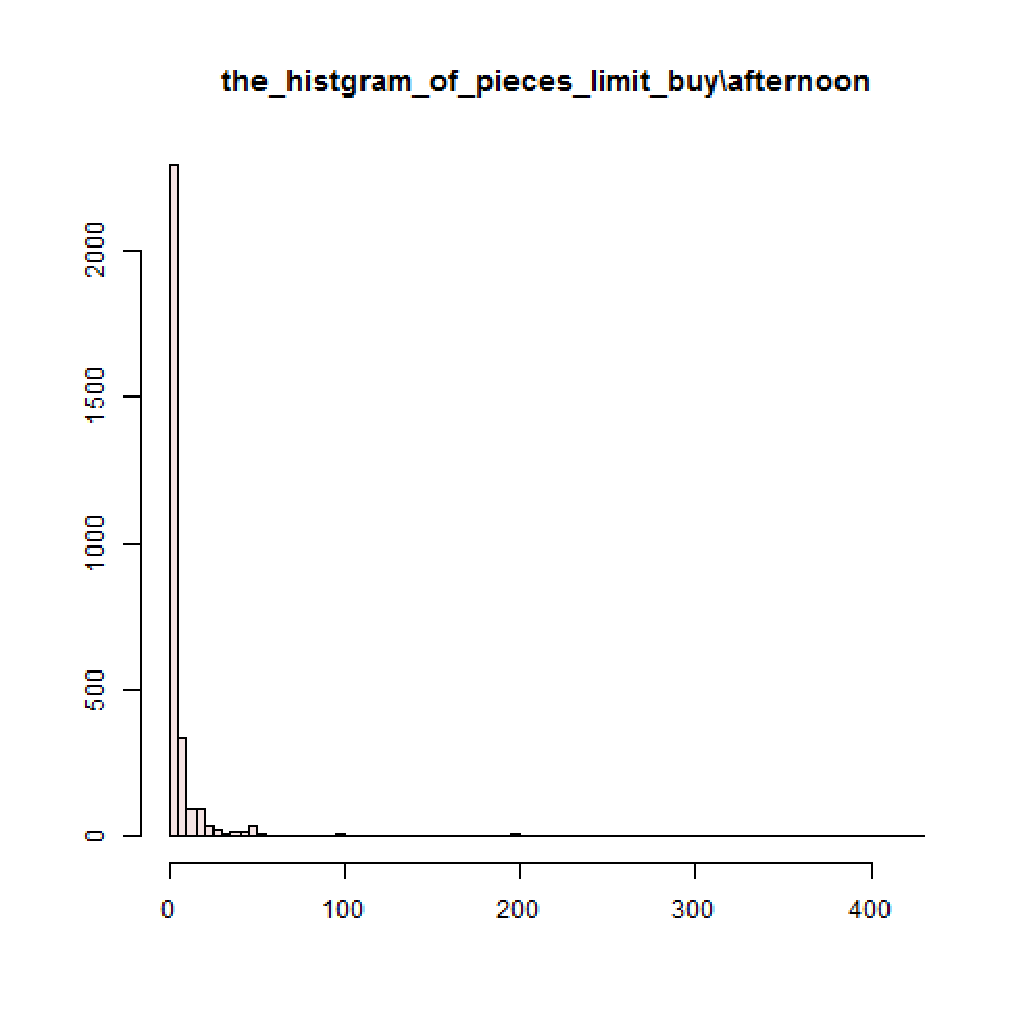
\includegraphics[clip,width = 5.0cm]{graphics/pieces_limit_buy20070129_.eps}
            \end{center}
            \caption{\scriptsize 買い指値注文の一回の注文枚数の頻度分布(2007年1月29日後場)}
        \end{minipage}
        \begin{minipage}{1\hsize}
        	\begin{center}
    			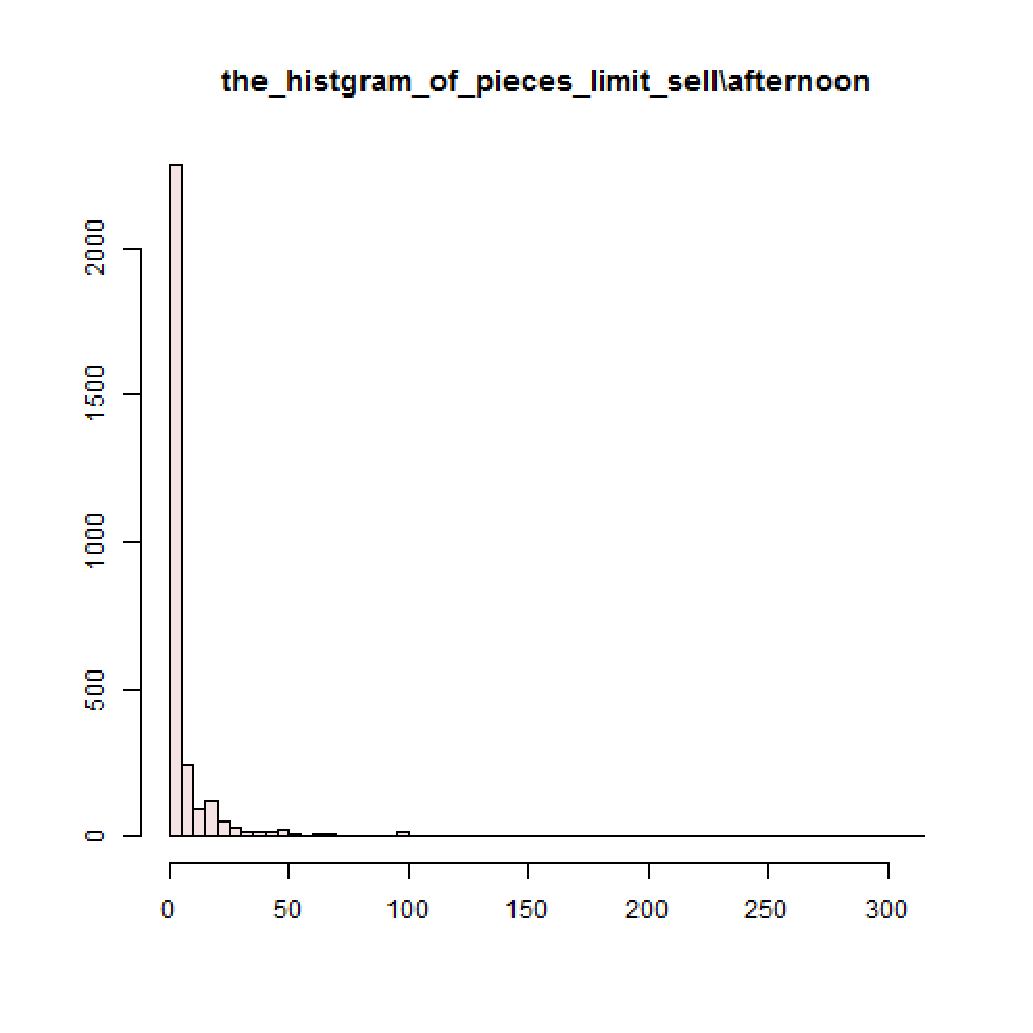
\includegraphics[clip,width = 5.0cm]{graphics/pieces_limit_sell20070129_.eps}
            \end{center}
            \caption{\scriptsize 売り指値注文の一回の注文枚数の頻度分布(2007年1月29日後場)}
        \end{minipage}
    \end{figure}
    \begin{figure}[H]
        \begin{minipage}{1\hsize}
        	\begin{center}
    			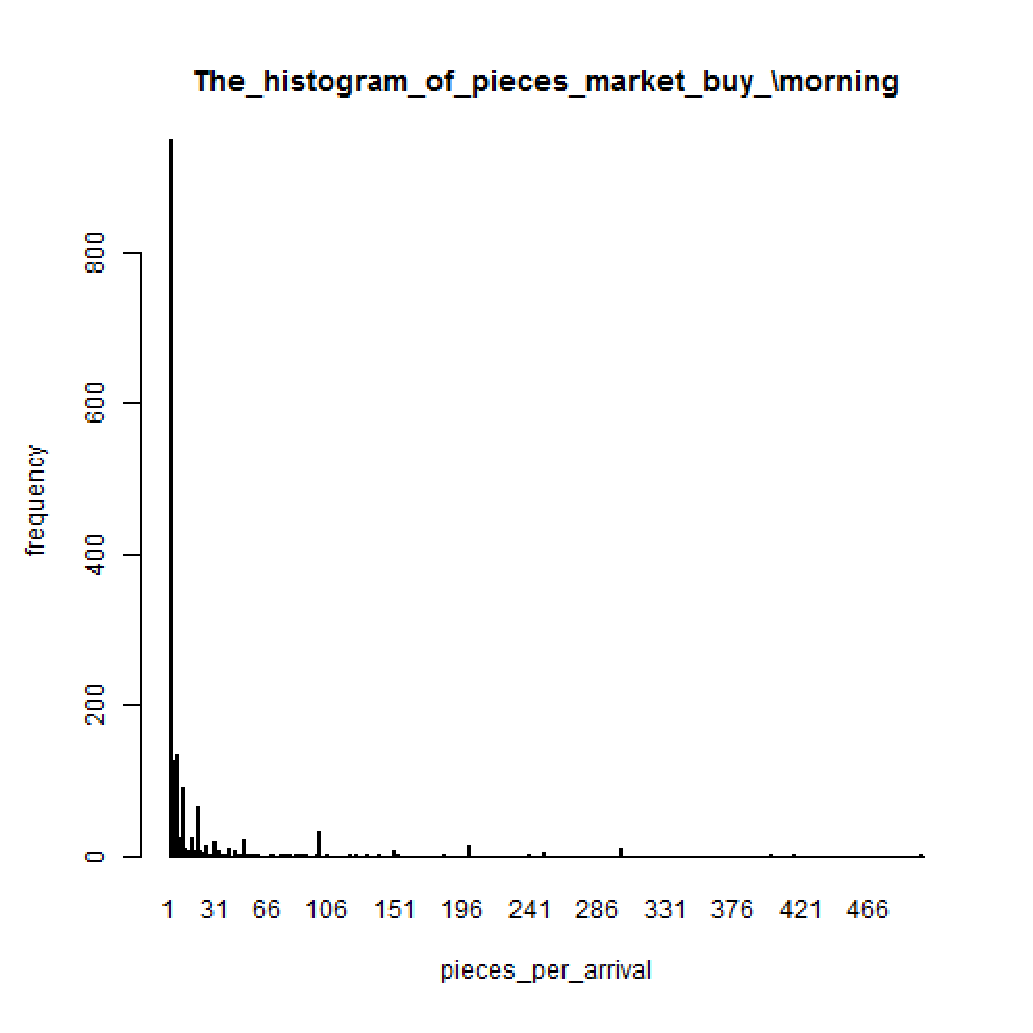
\includegraphics[clip,width = 5.0cm]{graphics/pieces_market_buy20070129_.eps}
            \end{center}
            \caption{\scriptsize 買い成行注文の一回の注文枚数の頻度分布(2007年1月29日後場)}
        \end{minipage}
        \begin{minipage}{1\hsize}
        	\begin{center}
    			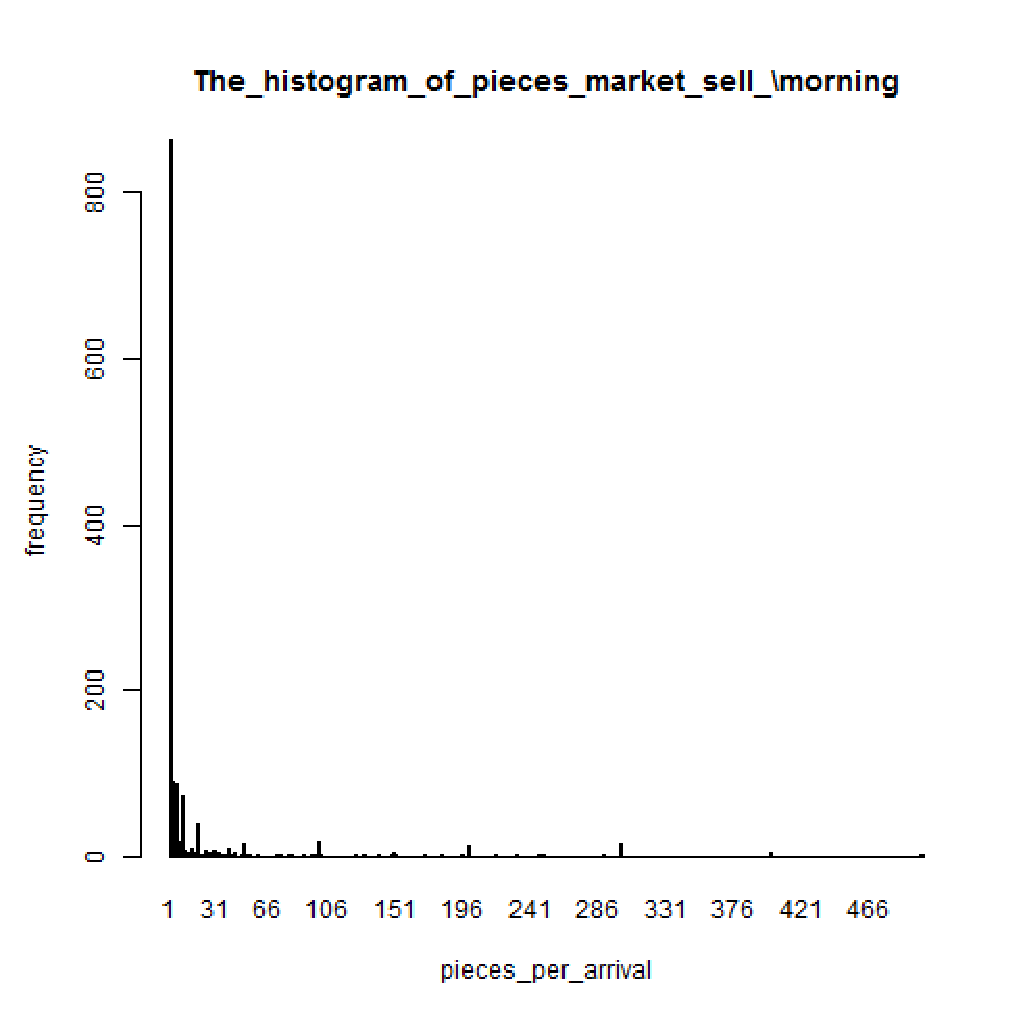
\includegraphics[clip,width = 5.0cm]{graphics/pieces_market_sell20070129_.eps}
            \end{center}
            \caption{\scriptsize 売り成行注文の一回の注文枚数の頻度分布(2007年1月29日後場)}
        \end{minipage}
    \end{figure}
    
    %到着数の統計量
    到着は小さい数字への偏りがかなり大きい.キリの良い数字($1,2,5,10,15,20,25,30,50,100,\cdots$)の注文枚数が多くなる傾向が見られる.
    
    ひとまずは一回の指値/成行の注文数は平均株数を一単位と考える(\cite{endo_zuo_kishimoto}と\cite{li_hui_endo_kishimoto}に倣う).板の解析は初期値(上下最良気配板の移動直後の板の厚み)から
    上下どちらかの板の厚みが$0$になるまでの厚みの変動を一つの待ち行列と見做し,板の移動毎にシステムが入れ替わると考える(前章までの理論部分では系内客数が$0$になってからも同一
    システム内の待ち行列を考えていた.注文時間間隔については架空サービスに対応する架空の注文を考える必要はない.).従って,注文の時間間隔を実データから抽出する際に注意するべきは,
    板の移動直前の最終の変化から板の移動が起こるまでの時間の扱いである.\\
    
    例えば最良買い気配について,板の動きの発生原因として考えられるのは次の四種類である.
    \begin{description}
    	\item[(1)] 最良買い気配数量が約定後に$0$になった場合
        \item[(2)] 最良売り気配数量が約定後に買い気配の方に飛び出した場合
    	\item[(3)] 最良気配板の幅が$2$ティック以上離れている下で,$1$ティック上に買い指値注文が来た場合
        \item[(4)] 注文がキャンセルされた場合
    \end{description}
    
    %板の移動の3パターン図
    
    抽出するべき時間間隔をまとめておく.
    \begin{table}[H]
    	\centering
    	\caption{抽出する指値/成行注文時間間隔}
        \begin{tabularx}{\linewidth}{l|X} \bhline{1.5pt}
    		観測開始点 & 板の移動直後の時間 \\ \hline \hline
        	最良気配値が変化するまで & 指値注文時間間隔,成行注文時間間隔$^\dagger$を抽出 \\ \hline \hline
        	最良買い気配値が下に移動した場合 & 移動直前に売りの成行注文があれば,その直近の売り成行注文から移動するまでの時間間隔を抽出 \\ \hline
        	最良売り気配値が上に移動した場合 & 移動直前に買いの成行注文があれば,その直近の買い成行注文から移動するまでの時間間隔を抽出 \\ \bhline{1.5pt}
        \end{tabularx}
        ({\footnotesize $\dagger$ 最良気配値にかかる数量が増加したら指値注文と判定する.減少したら,直前に約定があった場合のみ成行注文と判定する.})
    \end{table}
    
    この表に従って注文時間間隔を抽出する.
    
    また本研究では最良気配板の幅は常に$1$ティックであると仮定する.この仮定の妥当性のために$2$ティック以上離れている場合の時間が実際にどの程度なものであるかを示しておく.\\
    \begin{table}[H]
    	\centering
        \caption{最良気配値が$2$ティック以上離れている時間の割合(ザラバ時間全体を$1^\dagger$)}
        \small
        \begin{tabularx}{\linewidth}{l|lllll} \bhline{1.5pt}
        	 & {\rm Mean} & {\rm S.D.} & {\rm Median} & {\rm Minimum} & {\rm Maximum} \\ \hline
			$2006$ & $0.0195060586120777$ & $0.0677030612181418$ & $0.00208333333333333$ & $0$ & $0.444677871148459$ \\ \hline
			$2007$ & $0.0178285424121045$ & $0.0581349570904776$ & $0.00152777777777778$ & $0$ & $0.4403125$ \\ \hline
			$2008$ & $0.0332312105329688$ & $0.0880252112366147$ & $0.00168067226890756$ & $0$ & $0.502638888888889$ \\ \hline
			$2009$ & $0.0223041411093031$ & $0.0745940247185671$ & $0.000280112044817927$ & $0$ & $0.528645833333334$ \\ \hline
			$2010$ & $0.012512868645862$ & $0.0441851698948499$ & $0.000104166666666667$ & $0$ & $0.271666666666667$ \\ \hline
			$2011$ & $0.0091210487702376$ & $0.0348545571469177$ & $0.000135183850310542$ & $0$ & $0.293335736493489$ \\ \hline
			$2012$ & $0.0122896789716011$ & $0.0416945442875364$ & $0.000405441931705559$ & $0$ & $0.276624548736462$ \\ \hline
			$2013$ & $0.0185712489739548$ & $0.0612671979011189$ & $0.0018696636297624$ & $0$ & $0.51998377866895$ \\ \hline
			$2014$ & $0.0166132007108484$ & $0.0476355178792572$ & $0.000630687449319758$ & $0$ & $0.291937522571325$ \\ \hline
			$2015$ & $0.0213608996150105$ & $0.0656884482873762$ & $0.000180220770443794$ & $0$ & $0.385774209553012$ \\ \hline
			$2016$ & $0.0189805096200252$ & $0.0121494739702889$ & $0.0174577108570219$ & $0$ & $0.071640984049742$ \\ \bhline{1.5pt}
        \end{tabularx}
        ($\dagger$ 前場後場に分かれている日は前場後場それぞれのザラバの時間を$1$としている.)
    \end{table}

    
    $M/M/1$では到着時間間隔とサービス時間間隔が指数分布に従っていると仮定していた.注文時間間隔についてその仮定が妥当であるかどうかを調べる必要がある.
    分布の検定は$\chi^2$乗適合度検定による.検定の理論について%を参照されたい.\\
    帰無仮説は"実データの時間間隔が仮定する分布に従っていること"であり,棄却の有意水準は$5\%$とする.
    \begin{table}[H]
    	\centering
        \caption{検定の手順(有意水準$\alpha\ (0 < \alpha < 1)$)}
        \begin{tabularx}{\linewidth}{l|X} \bhline{1.5pt}
        	手順1 & 従っていると仮定する分布のパラメータの最尤推定量を計算する.\\ \hline
            手順2 & 時間間隔の区間を$[0, 1),[1, 2),[2, 3),\cdots,[9, 10),[10. \infty)$とし,実データの各時間間隔の頻度を計算する.\\ \hline
            手順3 & 最尤推定量をパラメータとする分布で各時間区間の確率を計算し,総データ数を掛けて頻度の理論値とする.\\ \hline
            手順4 & 各時間区間で\ $(\mbox{実現頻度-理論頻度})^2 / \mbox{理論頻度}$\ を計算,その総和が $\chi^2$ 検定等計量である.時間を$11$分割しているので,
            $2$を引いた数$9$が検定の自由度であり,その自由度の $\chi^2$ 分布の$(1-\alpha)$の確率点が検定統計量以下であれば帰無仮説を棄却する.\\ \bhline{1.5pt}
        \end{tabularx}
    \end{table}
            
    指数分布に従っていると仮定した下でのパラメータ$\lambda$と$\mu$の最尤推定量は,それぞれ$\ 1/\mbox{平均到着時間間隔}\ $,$1/\mbox{平均サービス時間間隔}\ $である.
    平均到着時間と平均サービス時間は各日の前場後場で別に計算し,分布の適合度の検定を各日の前場後場で別に行う.\\

\begin{comment}
\subsection{板の移動直後の最良気配の厚み}
	前節で述べた通り,板の移動毎にシステムが入れ替わると考える.これはどういうことか,板が移動するごとにシステムは新規の初期状態から始まるということある.
    この初期状態が板の移動直後の最良気配の厚みである.下図は板の移動直後の厚みの分布である.最良気配値の幅は常に$1$ティックと仮定して考えるから,
    ヒストグラム作成に用いた初期状態のデータはすべて最良気配値の幅は常に$1$ティックである時点のものである.
    %板の移動直後の絵
    
    板の移動直後の厚みの頻度分布を掲示しておく.
    
    ひとまずは,\cite{li_hui_endo_kishimoto}に倣ってこの初期状態はその平均値のみを取るものと考えておく.
\end{comment}

\subsection{モデルの変数と式}
	\cite{endo_zuo_kishimoto}と\cite{li_hui_endo_kishimoto}に倣ってモデルで使う変数を定義する.変数につける添え字$A$と$B$はそれぞれ$ask$と$bid$の意味である.
    この章のメインは稼動期間の章で導出した関数である.これは状態$i \geq 1$を初期状態とする$M/M/1$の待ち行列で,系内客数が$0$になるまでの時間の分布の確率密度関数であった.
    \begin{screen}
    	\begin{align}
    		r_i(t) &=
        	\begin{cases}	
        		\frac{i}{t} \exp{-(\lambda + \mu)t} \rho^{\frac{-i}{2}} I_{i}(2t\sqrt{\lambda \mu}) & (t > 0) \\
            	0 & (t \leq 0)
        	\end{cases} \quad (\rho = \lambda/\mu)\\
            &\mbox{$\lambda > 0:$\ 到着率,$\mu > 0:$\ サービス率,$i \geq 1:$\ 初期状態,$I_{k}(x):$\ 第一種変形{\rm Bessel}関数(定義は(\ref{sec:bessel_function})節).}
    	\end{align}
    \end{screen}
    ここで変数の定義を以下の通りとする:
    \begin{table}[H]
    \label{tb:def_parameters}
    	\centering
    	\caption{モデルで扱う変数の定義}
        \begin{tabularx}{\linewidth}{X|X} \bhline{1.5pt}
        	変数名 & 定義 \\ \hline \hline
    		$r_A$ & 最良売り気配数量の初期状態(板の移動直後の数量) \\ \hline
            $r_B$ & 最良買い気配数量の初期状態(板の移動直後の数量) \\ \hline
            $\lambda_A$ & 売り指値注文の到着率(1秒あたり到着数) \\ \hline
            $\lambda_B$ & 買い指値注文の到着率(1秒あたり到着数) \\ \hline
            $\mu_A$ & 買い成行注文の到着率(1秒あたり到着数) \\ \hline
            $\mu_B$ & 売り成行注文の到着率(1秒あたり到着数) \\ \hline
            $\rho_A$ & $\lambda_A / \mu_A$ \\ \hline
            $\rho_B$ & $\lambda_B / \mu_B$ \\ \hline
            $T_A$ & 最良売り気配数量が消滅するまでの時間 \\ \hline
            $T_B$ & 最良買い気配数量が消滅するまでの時間 \\ \bhline{1.5pt}
        \end{tabularx}
    \end{table}
    
    上記の変数を用いて最良気配の板が消滅するまでの時間の確率密度関数を表記する.
    \begin{align}
    	f_A(t) &\equiv 
        \begin{cases}
        		\frac{r_A}{t} \exp{-(\lambda_A + \mu_A)t} {\rho_A}^{\frac{-r_A}{2}} I_{r_A}(2t\sqrt{\lambda_A \mu_A}) & (t > 0) \\
            	0 & (t \leq 0)
        \end{cases},\\
        f_B(t) &\equiv 
        \begin{cases}
        		\frac{r_B}{t} \exp{-(\lambda_B + \mu_B)t} {\rho_B}^{\frac{-r_B}{2}} I_{r_B}(2t\sqrt{\lambda_B \mu_B}) & (t > 0) \\
            	0 & (t \leq 0)
        \end{cases}.
    \end{align}
    
    密度関数を用いて,板の消滅が有限時間内に発生する確率$\prob{T < \infty}$と消滅までの平均時間を次のように表すことができる.これらは
    指値と成行の注文の到着率の比$(\lambda/\mu)$によって場合分けされる.
    \begin{align}
    	\prob{T_A < \infty} &= \int_{0}^{\infty} f_A(t) dt =
        \begin{cases}
        	1. & \rho_A \leq 1  \\
            \rho_A^{-r_A}. & \rho_A > 1
        \end{cases} \\
        \prob{T_B < \infty} &= \int_{0}^{\infty} f_B(t) dt =
        \begin{cases}
        	1. & \rho_B \leq 1  \\
            \rho_B^{-r_B}. & \rho_B > 1
        \end{cases}
    \end{align}
    
    \begin{align}
    	\Exp{T_A} &= \begin{cases}
        	\frac{r_A}{\mu_A - \lambda_A}. & \rho_A < 1 \\
        	\infty. & \rho_A \geq 1
        \end{cases}\\
        \Exp{T_B} &= \begin{cases}
        	\frac{r_B}{\mu_B - \lambda_B}. & \rho_B < 1 \\
        	\infty. & \rho_B \geq 1
        \end{cases}
    \end{align}
    
    実際のデータから取り出した,指値/成行注文の頻度,一回の注文枚数,最良気配値の上昇/下降回数を表にしたものを掲示する.
    注文の頻度と板の上下変動回数については,各日の前場後場毎に数えられたものから平均,標準偏差などを計算している.
    \begin{table}[H]
    	\centering
        \caption{指値/成行注文の頻度, 一回の注文枚数, 最良気配値の上昇/下降回数\ ($2007$年)}
        \fontsize{6pt}\selectfont
    	\begin{tabularx}{\linewidth}{l||lllllll} \bhline{1.5pt}
        \label{tb:statistics_parameters}
        	 & {\rm Mean} & {\rm S.D.} & {\rm Median} & {\rm Kurtosis} & {\rm Skewness} & {\rm Minimum} & {\rm Maximum} \\ \hline \hline
			{\rm Arrival Frequency of Market Buy Orders} & $1874.57786885246$ & $907.484103685263$ & $1820.5$ & $5.1185084691139$ & $0.675534368239935$ & $71$ & $6361$ \\ \hline
			{\rm Arrival Frequency of Market sell Orders} & $1885.14344262295$ & $954.009590995031$ & $1821$ & $6.79165032585533$ & $0.984617354667294$ & $71$ & $8121$ \\ \hline
			{\rm Arrival Frequency of limit Buy Orders} & $3483.48360655738$ & $1120.23805942858$ & $3499.5$ & $3.82206042384918$ & $0.0599109340880956$ & $586$ & $7270$ \\ \hline
			{\rm Arrival Frequency of limit sell Orders} & $3394.53483606557$ & $1080.4145540672$ & $3368$ & $4.29653118280392$ & $0.18647765477941$ & $484$ & $8014$ \\ \hline
			{\rm Averege Pieces of One Market Buy Order} & $13.4276022948203$ & $3.02821244393427$ & $13.3429742057251$ & $3.04927526108989$ & $-0.216209540427003$ & $3.61744966442953$ & $21.3557291666667$ \\ \hline
			{\rm Averege Pieces of One Market sell Order} & $13.3293733928831$ & $3.20955218830292$ & $13.5109013640969$ & $3.06369808944509$ & $-0.460839652375353$ & $3.71140939597315$ & $20.4013819095477$ \\ \hline
			{\rm Averege Pieces of One limit Buy Order} & $8.52585676649367$ & $1.71382478337069$ & $8.20893204942981$ & $5.77743700031615$ & $1.36267116128345$ & $5.46618357487923$ & $16.2366456059736$ \\ \hline
			{\rm Averege Pieces of One limit sell Order} & $8.77484927828575$ & $1.97386833754685$ & $8.34547387331226$ & $5.07714586629268$ & $1.38186122218224$ & $5.31809065383073$ & $17.0588827377957$ \\ \hline
			{\rm Upmovement Times Of the Best Bid} & $120.293032786885$ & $75.1588474753461$ & $101$ & $14.0075069407575$ & $2.43433936442679$ & $17$ & $719$ \\ \hline
			{\rm Downmovement Times Of the Best Bid} & $120.715163934426$ & $76.4390136553141$ & $99.5$ & $15.4980786597166$ & $2.52544843838218$ & $16$ & $764$ \\ \hline
			{\rm Upmovement Times Of the Best Ask} & $119.084016393443$ & $74.072631475686$ & $100.5$ & $16.2491850829897$ & $2.59336838706365$ & $14$ & $749$ \\ \hline
			{\rm Downmovement Times Of the Best Ask} & $119.463114754098$ & $75.5175617154362$ & $99.5$ & $18.1165736972318$ & $2.71213913991385$ & $14$ & $794$ \\ \bhline{1.5pt}
        \end{tabularx}
    \end{table}
    
    表\ref{tb:def_parameters}に掲載したモデル式内のパラメータについても,実際のデータから抽出したものを掲示しておく.
    板の移動直後の板の厚み,すなわち待ち行列の初期状態を表すパラメータについて,\cite{li_hui_endo_kishimoto}では表\ref{tb:statistics_parameters}における一回あたりの到着枚数の平均
    ({\rm Averege Pieces of One limit(Market) Buy(sell) Order})を一単位として扱っているが,次の表には生データの単位($1$枚$=1000$株)で表示する.
    \begin{table}[H]
    	\centering
        \caption{最良気配の移動直後の最良気配の厚み(枚)\ ($2007$年)}
    	\begin{tabularx}{\linewidth}{l||llll} \bhline{1.5pt}
        	{\rm Initial Depth} & {\rm Best Ask (After Up)} & {\rm Best Bid (After Up)} & {\rm Best Ask (After Down)} & {\rm Best Bid (After Down)} \\ \hline \hline
            {\rm Mean} & $387.9131243$ & $34.14230907$ & $34.30352941$ & $387.5713182$ \\ \hline
            {\rm S.D.} & $226.3623811$ & $57.86859669$ & $58.08360898$ & $221.5858799$ \\ \bhline{1.5pt}
        \end{tabularx}
    \end{table}
    
    \begin{table}[H]
    	\centering
        \caption{指値/成行注文の到着率\ ($2007$年)}
        \scriptsize
    	\begin{tabularx}{\linewidth}{l||llllll} \bhline{1.5pt}
        \label{arrival_rate_per_second}
        	{\rm Arrival Rate Per Second} & \lambda_B & \lambda_A & \mu_A & \mu_B & \rho_B & \rho_A \\ \hline \hline
			{\rm Mean} & $0.445193022565915$ & $0.435345808209839$ & $0.242113490982135$ & $0.244110689423828$ & $2.0870484873252$ & $2.0823603295046$ \\ \hline
			{\rm S.D.} & $0.135971954891417$ & $0.130776581330922$ & $0.112304593281721$ & $0.117891721530976$ & $0.758709519340317$ & $0.939755925473787$ \\ \bhline{1.5pt}
        \end{tabularx}
    \end{table}
    
    表\ref{arrival_rate_per_second}の結果は\cite{li_hui_endo_kishimoto}の結果と大分違った.\cite{li_hui_endo_kishimoto}では到着率を分単位で計算していて,
    その結果は$\lambda_B=3.77, \lambda_A=3.72, \mu_A=4.71, \mu_B=4.65$である.今回の結果を$60$倍してもこの数字には近くない.また$\rho_A, \rho_B$が\cite{li_hui_endo_kishimoto}
    にては$1$未満であるものの,表\ref{arrival_rate_per_second}では$1$を超えている.但し,\cite{li_hui_endo_kishimoto}が基にしているデータ期間は$2006/12/11 \sim 2007/12/13$であり,
    今回のデータは$2007/01/04 \sim 2007/12/28$であるから,およそ$10$日間のズレがある.それでも計算された結果があまりにも違った.\\
    \mbox{}\\
    稼働時間$T_A,\ T_B$については次のようになる.これは$bid$と$ask$それぞれについて今の変動とその直前の変動の時間を抽出するのであるが,
    最良買い気配値で約定があった直後に板が下に動いた場合は最良買い気配の稼働時間として,
    最良売り気配値で約定があった直後に板が上に動いた場合は最良売り気配の稼働時間と判定している.各日の前場後場に分けて計算された記述統計量を掲示する.
    
    \begin{table}[H]
    	\centering
        \caption{稼働時間\ ($2007$年)}
        \begin{tabularx}{\linewidth}{l||ll} \bhline{1.5pt}
        	{\rm Operating Time} & $T_A$ & $T_B$ \\ \hline
			{\rm Mean} & $165.22340899656$ & $183.672253898271$ \\ \hline
			{\rm S.D.} & $211.849091373012$ & $217.626298979503$ \\ \hline
        \end{tabularx}
    \end{table}


%付録
\appendix
\section{{\rm Egorov}の定理}
\label{sec:appendix_egorov}
	\begin{screen}
    	\begin{Prop}
        	\begin{description}
            	\item[{\rm Egorov}の定理の補助定理]\mbox{}\\
        			測度空間を$({\rm X}, \mathfrak{B}, \mu)$とする.${\rm X}$で定義される$\mathfrak{B}-\mbox{可測関数}$の列$\{f_n(x)\}_{n=1}^{\infty}$は${\rm X}$上で有限であり
            		${\rm X}$の各点で有限な$f(x)$に収束すると仮定する.$\mu({\rm X})<\infty$が成り立っているとき,任意の$\epsilon > 0$と$\eta > 0$
            		に対して或る集合$F \in \mathfrak{B}$と自然数$N$が存在して,
            		\begin{align}
            			\mu(X - F) < \eta, \quad & \\
                		|f_n(x) - f(x)| < \epsilon, \quad & (\forall n \geq N,\quad \forall x \in F) & \label{eq:egorov_lemma}
            		\end{align}
            		が成り立つ.
            \end{description}
        \end{Prop}
    \end{screen}
    \begin{Proof}
    	\begin{align}
        	E_n \equiv \bigcap_{k=n}^{\infty} \{x \mid |f_k(x) - f(x)| < \epsilon\}
        \end{align}
        とおく.定義の仕方から集合列$\{E_n\}_{n=1}^{\infty}$は単調非減少列であり,$\{f_n(x)\}_{n=1}^{\infty}$の各点収束の仮定から
        $E_1 \subset E_2 \subset E_3 \subset \cdots \rightarrow {\rm X}$が成り立つ.(\quad$x \in {\rm X} \Rightarrow x \in E_n,\ (\exists n)\quad$と
        $\quad x \in \bigcup\limits_{n=1}^{\infty} E_n \Rightarrow x \in {\rm X}\quad$が云える事を確認すればよい.) \\
        測度の完全加法性から$\lim\limits_{n \to \infty} \mu(E_n) = \mu({\rm X})$が成り立ち,$\mu({\rm X})<\infty$の仮定から
        或る$N \in \mathbb{N}$が存在して,全ての$n \geq N$に対して$\mu({\rm X}) - \mu(E_n) < \eta$が成り立つ.$F \equiv E_N$と置けば
        $\{E_n\}_{n=1}^{\infty}$の単調性から式(\refeq{eq:egorov_lemma})が成り立つ.\qed
    \end{Proof}
    
    \begin{screen}
    	\begin{Prop}
        	\begin{description}
            	\item[{\rm Egorov}の定理]\mbox{}\\
                	測度空間を$({\rm X}, \mathfrak{B}, \mu)$とする.${\rm X}$で定義される$\mathfrak{B}-\mbox{可測関数}$の列$\{f_n(x)\}_{n=1}^{\infty}$は
            		${\rm X}$の殆どいたるところで有限な値を取り,${\rm X}$の殆どいたるところの各点で有限な$f(x)$に収束すると仮定する.
                    $\mu({\rm X})<\infty$が成り立っているとき,任意の$\nu > 0$に対して或る集合$H \in \mathfrak{B}$が存在して,
            		\begin{align}
            			\mu(X - H) < \nu
            		\end{align}
                    でかつ$F$の上で$\{f_n(x)\}_{n=1}^{\infty}$は$f(x)$に一様収束する.
            \end{description}
        \end{Prop}
    \end{screen}
    \begin{Proof}
        各$f_n(x)$の有限でない集合$E_{n0} \equiv \{x \mid f_n(x) = \infty \}$は$\mu$の零集合である.その合併集合$\bigcup\limits_{n=1}^{\infty} E_{n0}$
        もまた零集合であるからこれを除いて,もとより$\{f_n(x)\}_{n=1}^{\infty}$は${\rm X}$上で有限であり${\rm X}$の各点で有限な$f(x)$に収束すると仮定して良い.
        先の定理で$\epsilon = \frac{1}{2^m},\ \eta = \frac{\nu}{2^m},\quad (m = 1,2,3,\cdots)$とすれば,或る集合$H_m \in \mathfrak{B}$と自然数$N_m$が存在して
        \begin{align}
        	\mu(X - H_m) < \frac{\nu}{2^m}, \quad & \\
            |f_n(x) - f(x)| < \frac{1}{2^m}, \quad & (\forall n \geq N_m,\quad \forall x \in H_m) 
        \end{align}
        が成り立つ.$H \equiv \bigcap_{m=1}^{\infty} H_m$と置けば,
        \begin{align}
        	\mu(X - H) = \mu\left(X - \bigcap_{m=1}^{\infty} H_m\right) = \mu \left(\bigcup_{m=1}^{\infty} (X - H_m) \right) < \sum_{m=1}^{\infty} \frac{\nu}{2^m} = \nu
        \end{align}
        が成り立ち,かつ$H$の上では任意の$\epsilon > 0$に対して$\frac{1}{2^m} < \epsilon$を満たすような$m$に対応する$N_m$に対し,
        \begin{align}
        	|f_n(x) - f(x)| < \epsilon, \qquad (\forall n \geq N_m)
        \end{align}
        とできる.即ち可測関数列$\{f_n(x)\}_{n=1}^{\infty}$が一様収束すると示された.
    	\qed
    \end{Proof}
    
    

\section{{\rm k-Erlang}分布の特性関数}
\label{sec:appendix_erlang}
	\begin{description}
    	\item[到着分布の例:{\rm k-}アーラン分布\ {\rm (k-Erlang\ distribution)}]\mbox{}\\
    		\begin{align}
    			E_k(x) \equiv
        		\begin{cases}
        			1 - \exp{-\lambda k x} \left( 1 + \frac{\lambda k x}{1!} + \cdots + \frac{(\lambda k x)^{k-1}}{(k-1)!} \right) & \text{$x \geq 0$}\\
    				0 & \text{$x < 0$}
        		\end{cases}
    		\end{align}
        平均,分散,特性関数を計算する.
        密度関数
        \begin{align}
            f(x) &= E_k'(x) \\&= 
            \begin{cases}
        			\lambda k \exp{-\lambda k x} \left( 1 + \frac{\lambda k x}{1!} + \cdots + \frac{(\lambda k x)^{k-1}}{(k-1)!} \right)
                    - \lambda k \exp{-\lambda k x} \left( 1 + \frac{\lambda k x}{1!} + \cdots + \frac{(\lambda k x)^{k-2}}{(k-2)!} \right) & \text{$x \geq 0$}\\
    				0 & \text{$x < 0$}
        	\end{cases} 
            \\&=
            \begin{cases}
        			\lambda k \exp{-\lambda k x} \frac{(\lambda k x)^{k-1}}{(k-1)!} & \text{$x \geq 0$}\\
    				0 & \text{$x < 0$}
        	\end{cases}.
        \end{align}
        これは{\rm Gamma}分布\ $G_A(k, \frac{1}{\lambda k})$の密度関数である.従って一般の
        {\rm Gamma}分布\ $G_A(\alpha, \beta)$について平均,分散,特性関数を計算する方が楽である.\\
        特性関数 : 確率変数 $X \sim G_A(\alpha, \beta)$ について,$\alpha > 1$として特性関数を導出する.
        \begin{align}
			\phi(t) &= E[e^{itX}] \\
			&= \int_{0}^{\infty} e^{itx} \frac{1}{\Gamma(\alpha)\beta^\alpha} x^{\alpha-1} e^{-\frac{x}{\beta}} dx \\
			&= \int_{0}^{\infty} \frac{1}{\Gamma(\alpha)\beta^\alpha} x^{\alpha-1} e^{-\left(\frac{1}{\beta}-it\right)x} dx	\\
			&= \lim_{R \to \infty} \int_{0}^{R} \frac{1}{\Gamma(\alpha)\beta^\alpha} x^{\alpha-1} e^{-\left(\frac{1}{\beta}-it\right)x} dx \\
			&= \lim_{R \to \infty} \frac{1}{\Gamma(\alpha)\beta^\alpha} \left(\frac{\beta}{1-i \beta t}\right)^\alpha \int_{0}^{\frac{R}{\beta}-itR} z^{\alpha-1} e^{-z} dz.
		\end{align}
        ここで
		\begin{align}
			\int_{0}^{\frac{R}{\beta}-itR} z^{\alpha-1} e^{-z} dz
		\end{align}
		について複素積分を考える.
        
        \begin{picture}(300,210)(0,0)
        	\put( 30,  0){\vector(0,1){200}}
            \put(  0,180){\vector(1,0){300}}
            \thicklines
            \put(230,180){\vector(-1,0){100}}
            \put(130,180){\line(-1,0){100}}
            \put(230, 30){\vector(0,1){70}}
            \put(230,100){\line(0,1){80}}
            \put( 30,180){\vector(4,-3){200}}
            \multiput( 30, 30)(2,0){100}{\line(1,0){0.1}}
            \put( 20,170){$\mathsrc{O}$}
            \put(290,185){$\mathsrc{Re}$}
            \put( 20,200){$\mathsrc{Im}$}
            \put(100,185){$\Gamma_3$}
            \put(235,100){$\Gamma_2$}
            \put(100, 90){$\Gamma_1$}
            \put(230,185){$\frac{R}{\beta}$}
            \put(  5, 30){$-itR$}
        \end{picture}
        
        積分路を$\Gamma \equiv \Gamma_1 \cup \Gamma_2 \cup \Gamma_3$として,被積分関数が$\mathbb{C}$の整関数であることから$\Gamma$および内部領域に孤立特異点は存在しない.
		積分の向きは左回りとして,{\rm Cauchy}の積分定理が成り立つので
		\begin{align}
			\oint_{\Gamma} z^{\alpha-1} e^{-z} dz = 0
		\end{align}
		が成り立つ.
		$\Gamma_2$上の積分は
		\begin{align}
			\left| \int_{\Gamma_2} z^{\alpha-1} \exp{-z} dz \right| 
            &= \left| \int_{-tR}^{0} \left(\frac{R}{\beta}+iy\right)^{\alpha-1} \exp{-\frac{R}{\beta}-iy} i dy \right| \\
			&\leq \int_{-tR}^{0} \left(\frac{R}{\beta}+|y|\right)^{\alpha-1} \exp{-\frac{R}{\beta}} dy.
		\end{align}
		任意の$\epsilon > 0$に対し$t$について定まる或る$R_1(t)$が存在して,$R > R_1(t)$ならば
		\begin{align}
			\int_{-tR}^{0} \left(\frac{R}{\beta}+|y|\right)^{\alpha-1} e^{-\frac{R}{\beta}} dy < \epsilon
		\end{align}
		が成り立つ.$\Gamma_3$上の積分は
		\begin{align}
			\int_{\Gamma_3} z^{\alpha-1} e^{-z} dz = \int_{\frac{R}{\beta}}^{0} z^{\alpha-1} e^{-z} dz = -\int_{0}^{\frac{R}{\beta}} z^{\alpha-1} e^{-z} dz.
		\end{align}
		これも広義積分は収束するので,任意の$\epsilon > 0$に対し或る$R_2$が存在して,$R > R_2$ならば
		\begin{align}
			\Gamma(\alpha)-\epsilon < \int_{0}^{\frac{R}{\beta}} z^{\alpha-1} e^{-z} dx \leq \Gamma(\alpha).
		\end{align}
		従って,$R > \max{R_1(t)}{R_2}$と置いて
		\begin{align}
			\left|\int_{\Gamma_1} z^{\alpha-1} e^{-z} dz -  \Gamma(\alpha)\right|
			&= \left|-\int_{\Gamma_2} z^{\alpha-1} e^{-z} dz
		    	   -\int_{\Gamma_3} z^{\alpha-1} e^{-z} dz - \Gamma(\alpha)\right| \\
            &= \left|\int_{\Gamma_2} z^{\alpha-1} e^{-z} dz \right| + \left| \int_{0}^{\frac{R}{\beta}} z^{\alpha-1} e^{-z} dz - \Gamma(\alpha)\right| \\
            &< 2 \epsilon.
		\end{align}
		$\epsilon$は任意であるから
		\begin{align}
			\lim_{R \to \infty} \frac{1}{\Gamma(\alpha)\beta^\alpha} \left(\frac{\beta}{1-i \beta t}\right)^\alpha \int_{0}^{\frac{R}{\beta}-itR} z^{\alpha-1} e^{-z} dz 
			= \left(\frac{1}{1-i \beta t}\right)^\alpha
		\end{align}
		が成り立つ.$t \leq 0$の場合も同じ結論となる.
        \qed
    \end{description}

\section{{\rm Glivenko}の定理}
\label{sec:glivenko_theorem}
	{\rm Glivenko}の定理を示すには若干多めの準備が必要である.特性関数の性質を述べる前に分布の収束についての同値条件の定理から示す.
    そのためには{\rm Lindel$\ddot{o}$f}の被覆定理が必要で,この点に関して参照した教科書にはない証明を加えるので,確率論の勉強のためにも
    この章は少し有用である.次に特性関数に関するいくつかの特徴を述べた後に{\rm Glibenko}の定理を証明してこの章を終わる.
    伊藤清「確率論」第$2$章と伊藤清三「ルベーグ積分入門」付録$2$章を参照されたい.
\subsection{{\rm Lindel$\ddot{o}$f}の被覆定理}
	有理数が可算集合であることは以下のように考えればわかる.\\
    有理数は自然数同士の分数$p/q,\quad (p,q \in \mathbb{N})$で表される.ここで分母を行,分子を列の数字で表すように行列を考える.
    \begin{align}
    \arraycolsep5pt
    	\left(
    	\begin{array}{@{\,}c|cccccc@{\,}}
    		&1&2&3&4&5&\cdots\\
    		\hline
    		1&1/1&1/2&1/3&1/4&1/5&\cdots\\
    		2&2/1&2/2&2/3&2/4&2/5&\cdots\\
    		3&3/1&3/2&3/3&3/4&3/5&\cdots\\
    		4&4/1&4/2&4/3&4/4&4/5&\cdots\\
    		5&5/1&5/2&5/3&5/4&5/5&\cdots\\
    		\vdots&\vdots&\vdots&\vdots&\vdots&\vdots&\ddots\\
    	\end{array}
    	\right)
    \end{align}
    この行列の全成分は$\mathbb{R}$の有理数全体である.この成分全てをめぐり且つ自然数と対応を付けるとしたら,
    分母と分子の和が等しい箇所同士(行列を左斜め向きに見る)で順に番号を付ければばよい.
    \begin{align}
    	1/1 &&\to 1/2 &&\to 2/1 &&\to 1/3 &&\to 2/2 &&\to 3/1 &&\to \cdots, \\
        \Rightarrow a_1 &&\to a_2 &&\to a_3 &&\to a_4 &&\to a_5 &&\to a_6 &&\to \cdots. \\
    \end{align}
    負数ももちろん考慮する必要がある.絶対値が同じものを正数と負数で交互に並べればよい.
    \begin{align}
        a_1 &&\to -a_1 &&\to a_2 &&\to -a_2 &&\to a_3 &&\to -a_3 &&\to a_4 &&\to -a_4 &&\to \cdots,\\
        \Rightarrow b_1 &&\to b_2 &&\to b_3 &&\to b_4 &&\to b_5 &&\to b_6 &&\to b_7 &&\to b_8 &&\to \cdots.
    \end{align}
    \begin{screen}
    	\begin{Prop}
        	$N$次元実数空間$\mathbb{R}^N$における有理点全体は可算集合である.
        \end{Prop}
    \end{screen}
    \begin{Proof}
    	$\mathbb{R}^1$の有理数の全体を$Q \equiv \{r_m\}_{m=1}^{\infty} = \{ r_1, r_2, r_3, r_4, r_5, \cdots \}$で表す.
        $\mathbb{R}^N$の有理点は$Q$から任意に$N$個の有理数を選んでできるから,選ばれる添え字集合を
        $\{ m_{(1)}, m_{(2)}, m_{(3)}, \cdots, m_{(N)} \}$と表す.添え字集合の和に注目して,
        \begin{align}
        	Q_N \equiv \bigcup_{k=N}^{\infty} \left\{ ( r_m_{(1)}, r_m_{(2)}, r_m_{(3)}, \cdots, r_m_{(N)})\ \middle|\ \sum_{t=1}^{N} m_{(t)} = k \right\}
        \end{align}
        とすれば,$Q_N$は$\mathbb{R}^N$における有理点の全体を表現し,各$k$に対して$\left\{ ( r_m_{(1)}, r_m_{(2)}, r_m_{(3)}, \cdots, r_m_{(N)})\ \middle|\ \sum_{t=1}^{N} m_{(t)} = k \right\}$
        は有限集合であるから$Q_N$は可算集合であると判る.\qed
    \end{Proof}
    
    \begin{screen}
    	\begin{description}
        	\item[$\mathbb{R}$における稠密{\rm (dense)}]\mbox{}\\
            $\mathbb{R}$の集合$C$が稠密であるとは,任意の$x \in \mathbb{R}$の任意の近傍を取ったときに,$C$の点がその近傍の内部に少なくとも一つ含まれることを云う.
        \end{description}
    \end{screen}
    
    \begin{screen}
    	\begin{Prop}
        	$N$次元実数空間$\mathbb{R}^N$における有理点全体$Q_N = \{ x_1, x_2, x_3, x_4, x_5, \cdots \}$は$\mathbb{R}^N$で稠密な集合である.
        \end{Prop}
    \end{screen}
    \begin{Proof}
    	有理数全体$Q$が$\mathbb{R}^1$で稠密であることは次のようにして示される.\\
        実数全体は有理数と無理数に分けられる.任意の無理数に対しそれが有理数の集積点であることを言えばよい.$x$を任意の無理数とせよ.
        $x$を内部に含む有理数の区間$(r_1, r_2)$を取る.$r_1$と$r_2$の中点$r_3$も有理数であるから,$x$は$(r_1, r_3)$か$(r_3, r_2)$のどちらかの内点となる.
        $x$が含まれる方の区間で再び中点を取りそれを$r_4$と表す.$x$を内部に含む区間を作る操作を繰り返し点列$\{r_n\}_{n=1}^{\infty}$を構成すると,
        $r_n$と$x$の距離は$|x - r_n| < (r_2 - r_1)/2^{n-2} \quad (n = 3,4,5,\cdots)$の不等式を満たすから,点列$\{r_n\}_{n=1}^{\infty}$は$x$への収束点列であると判る.
        即ち有理数全体$Q$は$\mathbb{R}^1$で稠密である.\\
        次に有理点全体$Q_N$が$\mathbb{R}^N$で稠密であることを示す.任意の$x \in \mathbb{R}^N$を成分に分解する:\\
        $x= (x_1, x_2, x_3, \cdots , x_N)$と表す.任意の$\epsilon > 0$について$x$の$\epsilon$近傍${\rm U}(x, \epsilon)$の内部に少なくとも一点の有理点が存在することを示せばよい.
        $x$の各成分$x_i\ (i=1,2,3,\cdots,N)$からその$x_i$軸方向に対し距離$\delta < \epsilon/\sqrt{N}$内の区間$(x_i, x_i + \delta)$の内部には少なくとも一つの有理数$r_{(i)}$が含まれる.
        各軸の上の有理数$r_{(i)},\ (i=1,2,3,\cdots,N)$で構成される点$(r_{(1)}, r_{(2)}, r_{(3)}, \cdots, r_{(N)})$は有理点であり${\rm U}(x, \epsilon)$の内点でもある.
        したがって有理点全体$Q_N$は$\mathbb{R}^N$で稠密であると証明された.\qed
    \end{Proof}
    
    \begin{screen}
    	\begin{Prop}
        	$N$次元実数空間$\mathbb{R}^N$における有理点全体を$Q_N = \{ x_1, x_2, x_3, x_4, x_5, \cdots \}$,$\mathbb{R}^1$の有理数の全体を$Q = \{ r_1, r_2, r_3, r_4, r_5, \cdots \}$で表し,
            有理点を中心とし有理数を半径とする開球全体を$\{{\rm U}(x_p, r_q) \mid p,q \in \mathbb{N} \}$と表す.$\mathbb{R}^N$の任意の開集合$G$に対し,$G$に含まれるような${\rm U}(x_p, r_q)$の全体を
            $\{ {\rm U}_1, {\rm U}_2, {\rm U}_3, \cdots \}$とすると,
            \begin{align}
            	G = \bigcup_{n=1}^{\infty} {\rm U}_n
            \end{align}
            が成り立つ.
        \end{Prop}
    \end{screen}
    \begin{Proof}
    	$\{ {\rm U}_1, {\rm U}_2, {\rm U}_3, \cdots \}$の選び方から$\bigcup_{n=1}^{\infty} {\rm U}_n \subset G$は明らかである.逆の関係を示せばよい.\\
        任意の$x \in G$には或る近傍${\rm U}(x, \delta)$が存在して${\rm U}(x, \delta) \subset G$を満たす.前定理により$Q_N$は$\mathbb{R}^N$で稠密であるから,少なくとも一つの
        $x_p \in Q_N$は${\rm U}(x, \delta/3)$に含まれる.有理数は$\mathbb{R}^1$で稠密であるから,少なくとも一つの$r_q \in Q$は$\delta/3 < r_q < 2\delta/3$を満たす.
        $\Norm{x_p - x} < \delta/3 < r_q$であるから$x \in {\rm U}(x_p, r_q)$が成り立ち,また$\Norm{x_p - x} + r_q < \delta/3 + 2\delta/3 = \delta$であるから
        ${\rm U}(x_p, r_q) \subset {\rm U}(x, \delta) \subset G$も成り立つ.従って${\rm U}(x_p, r_q)$は$\{ {\rm U}_1, {\rm U}_2, {\rm U}_3, \cdots \}$の要素である.
        $G$の任意の点は$\{ {\rm U}_1, {\rm U}_2, {\rm U}_3, \cdots \}$のいずれかには含まれると判明したから,$G \subset \bigcup_{n=1}^{\infty} {\rm U}_n$が示された.\qed
    \end{Proof}
    
    \begin{screen}
    	\begin{Prop}
        	{\rm Lindel$\ddot{o}$f}の被覆定理\mbox{}\\
            $E$を$\mathbb{R}^N$に含まれる任意の集合とする.$E$を覆う開被覆の系$\{ G_\lambda \}_{\lambda \in \Lambda},\ (\Lambda \mbox{はなんらかの添え字集合})$が存在して
            \begin{align}
            	E \subset \bigcup_{\lambda \in \Lambda} G_\lambda
            \end{align}
            が成り立つなら,そのうちの高々可算無限個の系列$\{G_\lambda_n\}_{n=1}^{\infty}$で$E$を覆うことができる.
        \end{Prop}
    \end{screen}
    \begin{Proof}
    	前定理より,任意の開集合$G_\lambda$は有理点を中心する半径が有理数の開球の和集合で置き換えることができる:
        \begin{align}
        	G_\lambda = \bigcup_{k=1}^{\infty} {\rm U}_{\lambda_k}, \quad ({\rm U}_{\lambda_k}\mbox{は前定理の${\rm U}(x_p, r_q)$の形式で表される}).
        \end{align}
        ところで$\{{\rm U}(x_p, r_q) \mid x_p \in Q_N,\ r_q \in Q\}$は可算集合であるから,$\bigcup_{\lambda \in \Lambda} G_\lambda$も可算集合である.従って
        $\left\{ {\rm U}_{\lambda_k}\ \middle|\ \lambda \in \Lambda,\ k=1,2,3,\cdots \right\}$の添え字を付け直し,
        $\left\{ {\rm U}_{\lambda_k}\ \middle|\ \lambda \in \Lambda,\ k=1,2,3,\cdots \right\} = \{V_n\}_{n=1}^{\infty}$と表すことができる.
        各$V_n$について,それを含む$G_\lambda$を一つ対応させ,それを$G_\lambda_n$と表記すれば,このように構成される可算個の開集合の系列
        $\{G_\lambda_n\}_{n=1}^{\infty}$によって$E$は覆われる.\qed
    \end{Proof}

\subsection{分布列の収束}
	分布$\mu$は$\mathbb{R}^1$の{\rm Lebesgue}可測な確率測度と考えよ:\\
    $\mathfrak{B}$を$\mathbb{R}^1$における{\rm Borel}集合とする.{\rm Lebesgue}可測な測度は{\rm Borel}可測な測度の完備化されたものである.
    \begin{align}
    	(1) &\quad \mu(\emptyset) = 0,\\
        (2) &\quad \forall E \in \mathfrak{B}, \quad 0 \leq \mu(E) \leq 1,\\
        (3) &\quad E_1,E_2,E_3,\cdots \in \mathfrak{B},\quad \mu\left(\sum_{n=1}^{\infty} E_n\right) = \sum_{n=1}^{\infty} \mu(E_n).
    \end{align}
    分布$\mu$に対応する分布関数$F(x)$は次のように定義される.
    \begin{align}
    	F(x) \equiv \mu((-\infty, x]).
    \end{align}
    \begin{screen}
    	\begin{description}
        	\item[連続点]\mbox{}\\
        		$\mu(\{x\}) = 0$を満たす点$x \in \mathbb{R}^1$を分布$\mu$の連続点と云う.これは分布関数$F$の連続点である.
            \item[不連続点]\mbox{}\\
            	$\mu(\{x\}) > 0$を満たす点$x \in \mathbb{R}^1$を分布$\mu$の不連続点と云う.これは分布関数$F$の飛躍点である.
        \end{description}
    \end{screen}
    \begin{screen}
    	\begin{description}
        	\item[分布列の収束]\mbox{}\\
            \label{def:convergence_distribution}
    			分布列$\{ \mu_n \}_{n=1}^{\infty}$が収束するとは,任意の有界実連続関数$f$に対して
    			\begin{align}
    				\lim_{n \to \infty} \int_{\mathbb{R}^1} f(x) \mu_n(dx) = \int_{\mathbb{R}^1} f(x) \mu(dx)
    			\end{align}
    			が成り立つことを云う.これを$\mu_n \to \mu$と表記する.
        \end{description}
    \end{screen}
    
    \begin{screen}
    	\begin{Prop}
        \label{Prop:convergence_distribution}
        	$\mu$を分布,$\{ \mu_n \}_{n=1}^{\infty}$を分布列,対応する分布関数をそれぞれ$F(x),\ F_n(x)\ (n=1,2,3,\cdots)$とする.
        	次に示す$(1)-(5)$は同値である.
            \begin{description}
            	\item[(1)]\qquad  $\mu_n \to \mu$.
                \item[(2)]\qquad 任意のコンパクトな台を有つ実連続関数$g(x)$に対して,
                	\begin{align}
                		\lim_{n \to \infty} \int_{\mathbb{R}^1} g(x) \mu_n(dx) = \int_{\mathbb{R}^1} g(x) \mu(dx).
                	\end{align}
                \item[(3)]\qquad $E \in \mathfrak{B}$に対して,その開核と閉包を$E^O$と$\overline{E}$で表す.$\mu(E^O) = \mu(\overline{E})$を満たす全ての$E \in \mathfrak{B}$に対して
                	\begin{align}
                		\lim_{n \to \infty} \mu_n(E) = \mu(E).
                	\end{align}
                \item[(4)]\qquad $F(x)$の全ての連続点$x$で
                	\begin{align}
                		\lim_{n \to \infty} F_n(x) = F(x).
                	\end{align}
                \item[(5)]\qquad $\mathbb{R}^1$の或る稠密な可算集合$C$が存在して,全ての$x \in C$で
                	\begin{align}
                    	\lim_{n \to \infty} F_n(x) = F(x).
                	\end{align}
            \end{description}
        \end{Prop}
    \end{screen}
    \begin{Proof}
    	証明の順番は$\quad (3) \to (4) \to (5) \to (2) \to (1) \to (3) \quad$である.
        \begin{description}
        	\item[{\large (3) \to (4)}]\mbox{}\\
            	$E = (-\infty, x] (\in \mathfrak{B})$と置く.$E^O = (-\infty, x),\quad \overline{E} = E$であるから,
                (3)を仮定すれば,$\mu((-\infty, x)) = \mu((-\infty, x])$を満たす全ての点$x$について
                \begin{align}
                	\lim_{n \to \infty} \mu_n((-\infty, x]) = \mu((-\infty, x])
                \end{align}
                が成り立つ.$\mu((-\infty, x]) - \mu((-\infty, x)) = \mu(\{x\}) = 0$を満たす点$x$は分布関数$F$の連続点であり,(3)は$F$の全ての連続点で上式が成り立つことを云っているのである.
                $F_n(x) = \mu_n((-\infty, x]),\quad F(x) = \mu((-\infty, x])$で上式を置き換えれば(4)が成立する.
            \item[{\large (4) \to (5)}]\mbox{}\\
            	$F(x)$の連続点集合の点から$\mathbb{R}^1$で稠密な可算集合を構成できることを示せばよい.\\
                その前に$F(x)$の不連続点集合が高々可算無限集合であることを示しておく.\\
                分布関数$F(x)$は$0 \leq F(x) \leq 1$を満たす単調非減少関数である.したがって高さ$1/n,\ (n=1,2,3,\cdots)$の飛躍がある不連続点は有限個しかない.
                $J_n,\ (n=1,2,3,\cdots)$を高さが$1/n$より大きい$F$の飛躍点集合であるとする.$F$の不連続点全体は$\bigcup_{n=1}^{\infty} J_n$で表され
                各$J_n$は有限集合であるから$F$の不連続点全体は高々可算無限集合である.\\
                即ち$F$の不連続点全体の{\rm Lebesgue}測度は$0$であり連続点全体は連続体濃度である.$F$の連続点全体を$C_F$,$F$の不連続点全体を$D_F$とおく.
                任意の$x \in C_F$に対しその$1/n$近傍を${\rm U}(x, 1/n)$と表す.$D_F$は可算集合だから
                \begin{align}
                	\mathbb{R}^1 \subset \bigcup_{x \in C_F} {\rm U}(x, 1/n)
                \end{align}
                が成り立つ.(成り立たないとすれば,それは$\mathbb{R}^1$の中に右辺で覆えない穴があるということであるが,その穴がある区間ならその中には$C_F$の点が無いと
                $D_F$が可算濃度であることに矛盾し,穴が一点であってそれが$D_F$の点であっても高々可算である以上その$1/n$近傍には$C_F$の点が無ければおかしい.)
                {\rm Lindel$\ddot{o}$f}の被覆定理により可算個の系列$\{{\rm U}(x_{n,k}, 1/n) \mid k=1,2,3,\cdots\}$の合併集合で$\mathbb{R}^1$を覆うことができる.(
                現時点では$n$を固定していることに注意.)
                そして$C_F$は連続体濃度であるから各$\{{\rm U}(x_{n,k}, 1/n)\}$の内部から$C_F$の点を取ることができる.その点を$y_{n,k}$と表す.
                $\{y_{n,k} \mid n=1,2,3,\cdots, k=1,2,3,\cdots\}$は可算集合であり,任意の$x \in \mathbb{R}^1$の任意の$\epsilon$近傍は(開集合であるから)適当な$(n,k)$による
                ${\rm U}(x_{n,k}, 1/n)$を含むから,必ず${\rm U}(x, \epsilon)$の内部に$\{y_{n,k} \mid n=1,2,3,\cdots, k=1,2,3,\cdots\}$の点が含まれる.
                以上より$\{y_{n,k} \mid n=1,2,3,\cdots, k=1,2,3,\cdots\}$は$\mathbb{R}^1$で稠密な可算集合であると示された.
            \item[{\large (5) \to (2)}]\mbox{}\\
            	(5)を仮定する.任意のコンパクトな台を有つ連続関数$g(x)$について,コンパクト集合上の連続関数は一様連続であるから有界である:
                \begin{align}
                	\forall x \in \mathbb{R}^1,\quad \exists M \in (0, \infty),\quad |g(x)| \leq M.
                \end{align}
                また任意の実数$a$に対して$\{x \mid g(x) < a\}$もまた開集合となるから$g(x)$は{\rm Borel}可測な関数である.従って$g(x)$に一様に近似できる左連続階段関数$g_\epsilon(x)$
                を構成することができる:
                \begin{align}
                	|g(x) - g_\epsilon(x)| < \frac{\epsilon}{3}, \quad (\forall x \in \mathbb{R}^1).
                \end{align}
                コンパクト集合の外側では$g_\epsilon(x)=0$と定義する.$g_\epsilon(x)$の飛躍点全体は可算集合でありこれを$\{ j_0, j_1, j_2, \cdots, j_m \}$と表す.この集合は(5)の仮定における可算集合$C$に含まれるとして問題ない.
                \begin{align}
                	\left| \int_{\mathbb{R}^1} g(x) \mu_n(dx) - \int_{\mathbb{R}^1} g(x) \mu(dx) \right| 
                    &= \left| \int_{\mathbb{R}^1} g(x) \mu_n(dx) - \int_{\mathbb{R}^1} g_\epsilon(x) \mu_n(dx) \right| \\
                    	&\quad+ \left| \int_{\mathbb{R}^1} g_\epsilon(x) \mu_n(dx) - \int_{\mathbb{R}^1} g_\epsilon(x) \mu(dx) \right| \\
                        &\quad+ \left| \int_{\mathbb{R}^1} g_\epsilon(x) \mu(dx) - \int_{\mathbb{R}^1} g(x) \mu(dx) \right| \\
                    &< \frac{2\epsilon}{3} + \left| \sum_{i=1}^{m}g_\epsilon(j_i)(F_n(j_i) - F_n(j_{i-1})) - \sum_{i=1}^{m}g_\epsilon(j_i)(F(j_i) - F(j_{i-1})) \right| \\
                    &\leq \frac{2\epsilon}{3} + \sum_{i=1}^{m}g_\epsilon(j_i) (| F_n(j_i) - F(j_i) | + | F_n(j_{i-1}) - F(j_{i-1}) |).
                \end{align}
                最終段第二項について,$\{ j_0, j_1, j_2, \cdots, j_m \}$は有限集合として取れる(仮に可算無限個取ったとせよ.飛躍点集合はコンパクト集合上に存在しているから,{\rm Bolzano-Weierstrass}
                の定理により$\{ j_0, j_1, j_2, \cdots\}$の中に集積点が存在する.集積点を$j_r$とでも表すと,$g(x)$の連続性から$j_r$の或る近傍を取れば関数値の変化量を$\epsilon$で抑えることができる.
                即ち$j_r$の或る近傍で無限個の飛躍を考える必要も無く$g_\epsilon(x)$を定義することができるので飛躍点は有限個で問題ない.)から$i$に関係なく或る$N \in \mathbb{N}$が取れて,全ての$n \geq N$に対して
                \begin{align}
                	\sum_{i=1}^{m}g_\epsilon(j_i) (| F_n(j_i) - F(j_i) | + | F_n(j_{i-1}) - F(j_{i-1}) |) < \frac{\epsilon}{3}
                \end{align}
                とできる.従ってこの$n,\ N$に対して以下が成り立つ:
                \begin{align}
                	\left| \int_{\mathbb{R}^1} g(x) \mu_n(dx) - \int_{\mathbb{R}^1} g(x) \mu(dx) \right| < \epsilon.
                \end{align}
            \item[{\large (2) \to (1)}]\mbox{}\\
            	$f(x)$を任意の有界実連続関数であるとする.任意の$m>0$に対し,コンパクト集合$[-m, m]$の上で$f$に一致,$[-m-1, m+1]^c$の上で$0$となり,$\mathbb{R}^1$全体で
                $0 \leq |g(x)| \leq |f(x)|$を満たす実連続関数$g(x)$を考える.
                
                \begin{picture}(280,50)(0,0)
                \put(0, 0){\vector(1,0){250}}
                \qbezier[100](0,10)(50,23)(100,20)
                \qbezier[100](100,20)(150,15)(200,25)
                \qbezier[50](200,25)(225,40)(250,35)
                \put(250,25){$f(x)$}
                \thicklines
                \qbezier(100,20)(150,15)(200,25)
                \put(100,20){\line(-1,-1){20}}
                \put(200,25){\line(4,-5){20}}
                \put(0,0){\line(1,0){80}}
                \put(220,0){\line(1,0){30}}
                \put(215,10){$g(x)$}
                \end{picture}
                
                \begin{align}
                	\left| \int_{\mathbb{R}^1} f(x)\mu_n(dx) - \int_{\mathbb{R}^1} f(x)\mu(dx) \right| 
                    &= \left| \int_{\mathbb{R}^1} f(x)\mu_n(dx) - \int_{\mathbb{R}^1} g(x)\mu_n(dx) \right| \\
                    	&\quad+ \left| \int_{\mathbb{R}^1} g(x)\mu_n(dx) - \int_{\mathbb{R}^1} g(x)\mu(dx) \right| \\
                        &\quad+ \left| \int_{\mathbb{R}^1} g(x)\mu(dx) - \int_{\mathbb{R}^1} f(x)\mu(dx) \right|.
                \end{align}
                右辺第二項は(2)の仮定により,任意の$\epsilon > 0$に対して或る$N_1 \in \mathbb{N}$が存在し,全ての$n \geq N_1$で
                \begin{align}
                	\left| \int_{\mathbb{R}^1} g(x)\mu_n(dx) - \int_{\mathbb{R}^1} g(x)\mu(dx) \right| < \frac{\epsilon}{4}
                \end{align}
                が成り立つ.第一項と第三項を考える前にもう一つ関数を用意する.
                コンパクト集合$[-m+1, m-1]$上で$0$,$[-m,m]^c$で$M$を取り,$\mathbb{R}^1$全体で$0 \leq |h(x)| \leq M$を満たす実連続関数$h(x)$を考える.
                
                \begin{picture}(280,60)(0,0)
                \put(0, 0){\vector(1,0){250}}
                \qbezier[100](0,10)(50,23)(100,20)
                \qbezier[100](100,20)(150,15)(200,25)
                \qbezier[50](200,25)(225,40)(250,35)
                \put(250,25){$f(x)$}
                \thicklines
                \qbezier(100,20)(150,15)(200,25)
                \put(100,20){\line(-1,-1){20}}
                \put(200,25){\line(4,-5){20}}
                \put(0,0){\line(1,0){80}}
                \put(220,0){\line(1,0){30}}
                \put(215,10){$g(x)$}
                
                \put(120,0){\line(-2,5){20}}
                \put(120,0){\line(1,0){60}}
                \put(180,0){\line(2,5){20}}
                \put(0,50){\line(1,0){100}}
                \put(200,50){\line(1,0){50}}
                \put(250,50){$h(x)$}
                \end{picture}
                
                \begin{align}
                	\left| \int_{\mathbb{R}^1} f(x)\mu_n(dx) - \int_{\mathbb{R}^1} g(x)\mu_n(dx) \right| 
                    &\leq \int_{\mathbb{R}^1} \left| f(x) - g(x) \right| \mu_n(dx) \\
                    &\leq \int_{\mathbb{R}^1} \left| h(x) \right| \mu_n(dx) \\
                    &= M - \int_{\mathbb{R}^1} (M - \left| h(x) \right|) \mu_n(dx).
                \end{align}
                ここで$(M - \left| h(x) \right|)$はコンパクトな台を有つ実連続関数であるから,(2)の仮定により
                或る$N_2 \in \mathbb{N}$が存在し,全ての$n \geq N_2$で
                \begin{align}
                	\left| \int_{\mathbb{R}^1} (M - \left| h(x) \right|) \mu_n(dx) - \int_{\mathbb{R}^1} (M - \left| h(x) \right|) \mu(dx) \right| < \frac{\epsilon}{4}
                \end{align}
                が成り立つ.これは即ち
                \begin{align}
                	\left| \int_{\mathbb{R}^1} \left| h(x) \right| \mu_n(dx) - \int_{\mathbb{R}^1} \left| h(x) \right| \mu(dx) \right| < \frac{\epsilon}{4}
                \end{align}
                が成り立つことと同じであり,
                \begin{align}
                	\left| \int_{\mathbb{R}^1} f(x)\mu_n(dx) - \int_{\mathbb{R}^1} g(x)\mu_n(dx) \right| 
                    \leq \int_{\mathbb{R}^1} \left| h(x) \right| \mu_n(dx)
                    < \int_{\mathbb{R}^1} \left| h(x) \right| \mu(dx) + \frac{\epsilon}{4}
                \end{align}
                とできる.
                \begin{align}
                	\int_{\mathbb{R}^1} \left| h(x) \right| \mu(dx) < M \mu([-m+1,m-1]^c) = M (1 - \mu([-m+1,m-1]))
                \end{align}
                について,$\mu$が確率測度であることから,或る$m'>0$が存在して,全ての$m \geq m'$に対して
                \begin{align}
                	M (1 - \mu([-m+1,m-1])) < \frac{\epsilon}{4}
                \end{align}
                が成り立つ.以上をまとめると,全ての$n \geq \max{N_1}{N_2}$と$m \geq m'$に対して
                \begin{align}
                	\left| \int_{\mathbb{R}^1} f(x)\mu_n(dx) - \int_{\mathbb{R}^1} f(x)\mu(dx) \right|  < \epsilon.
                \end{align}
            \item[{\large (1) \to (3)}]\mbox{}\\
            	$\mathbb{R}^1$の開区間は閉区間はそれぞれ閉集合の単調増加列,開集合の単調減少列の極限で表現できる.従って任意の{\rm Borel}集合$E$の開核$E^O$と閉包$\overline{E}$に対し
                或る閉集合$F_\epsilon\  (F_\epsilon \subset E^O)$と開集合$G_\epsilon\ (\overline{E} \subset G_\epsilon)$が存在して,測度の連続性から
                \begin{align}
                	\mu(E^O - F_\epsilon) < \epsilon,\qquad \mu(G_\epsilon - \overline{E}) < \epsilon
                \end{align}
                が成り立つ.(1)を仮定する.有界な連続実関数として,$F_\epsilon$の上で$1$,$E^O$の外側で$0$を取り,$\mathbb{R}^1$全体で$0 \leq f(x) \leq 1$を満たす
                関数を定義する.関数$f$と$\epsilon>0$に対して或る$N_1 \in \mathbb{N}$が存在して,全ての$n \geq N_1$で
                \begin{align}
                	\left| \int_{\mathbb{R}^1} f(x)\mu_n(dx) - \int_{\mathbb{R}^1} f(x)\mu(dx) \right| < \epsilon
                \end{align}
                が成り立つ.変形すれば
                \begin{align}
                	\mu(E^O) - 2\epsilon < \mu(F_\epsilon) - \epsilon < \int_{\mathbb{R}^1} f(x)\mu(dx) - \epsilon < \int_{\mathbb{R}^1} f(x)\mu_n(dx) \leq \mu_n(E^O).
                \end{align}
                同様に$\overline{E}$の上で$1$,$G_\epsilon$の外側で$0$を取り,$\mathbb{R}^1$全体で$0 \leq g(x) \leq 1$を満たす
                関数$g(x)$を定義する.関数$g$と$\epsilon > 0$に対して或る$N_2 \in \mathbb{N}$が存在して,全ての$n \geq N_2$で
                \begin{align}
                	\left| \int_{\mathbb{R}^1} g(x)\mu_n(dx) - \int_{\mathbb{R}^1} g(x)\mu(dx) \right| < \epsilon
                \end{align}
                が成り立つ.先ほどのように変形すれば
                \begin{align}
                	\mu_n(\overline{E}) < \int_{\mathbb{R}^1} g(x) \mu_n(dx) < \int_{\mathbb{R}^1} g(x) \mu(dx) + \epsilon < \mu(G_\epsilon) + \epsilon < \mu(\overline{E}) + 2\epsilon.
                \end{align}
                まとめると,全ての$n \geq \max{N_1}{N_2}$に対して
                \begin{align}
                	\mu(E^O) - 2\epsilon < \mu_n(E^O) \leq \mu_n(E) \leq \mu_n(\overline{E}) < \mu(\overline{E}) + 2\epsilon
                \end{align}
                が成り立つ.$\mu(E^O) = \mu(\overline{E})$であるならば(3)が成り立つことが示される.\qed
        \end{description}
    \end{Proof}

\subsection{特性関数}
    \begin{screen}
    	\begin{description}
        	\item[特性関数({\rm Characteristic\quad Function})]\mbox{}\\
            	分布$\mu$の特性関数$\phi(t),\ (-\infty < t < \infty)$は次のように定義される.
                \begin{align}
            		\phi(t) = \int_{\mathbb{R}^1} \exp{itx} \mu(dx).
                \end{align}
                $i$は虚数単位である.
        \end{description}
    \end{screen}
    \begin{screen}
    	\begin{Prop}
        	分布$\mu$の特性関数$\phi(t),\ (-\infty < t < \infty)$について,次の(1)-(3)が成り立つ.
            \begin{description}
            	\item[(1)] $\phi(0) = 1.$
            	\item[(2)] $\phi(t)$は正定({\rm Positive\quad Definite}).
            	\item[(3)] $\phi(t)$は$\mathbb{R}^1$で一様連続.
            \end{description}
        \end{Prop}
    \end{screen}
    \begin{Proof}
    	\begin{description}
        	$\phi(0) = \int_{\mathbb{R}^1} \exp{0} \mu(dx) = \mu(\mathbb{R}^1) = 1\quad$は定義から明らかである.\\
            正定であることを示す.$n$個の任意の複素数$\xi_1,\xi_2,\cdots,\xi_n \in \mathbb{C}^1$と
            $n$個の任意の実数$t_1,t_2,\cdots,t_n \in \mathbb{R}^1$とに対して,
            \begin{align}
            	\sum_{j,k=1}^{n} \xi_j \overline{\xi_k} \phi(t_j-t_k) &= \sum_{j,k=1}^{n} \xi_j \overline{\xi_k} \int_{\mathbb{R}^1} \exp{i(t_j-t_k)x} \mu(dx) \\
                &= \int_{\mathbb{R}^1} \sum_{j,k=1}^{n} \xi_j \overline{\xi_k} \exp{i(t_j-t_k)x} \mu(dx) \\
                &= \int_{\mathbb{R}^1} \sum_{j,k=1}^{n} \xi_j \exp{it_jx} \overline{\xi_k \exp{it_kx}} \mu(dx) \\
                &= \int_{\mathbb{R}^1} \sum_{j=1}^{n} \xi_j \exp{it_jx} \overline{\sum_{k=1}^{n} \xi_k \exp{it_kx}} \mu(dx) \\
                &= \int_{\mathbb{R}^1} \left| \sum_{j=1}^{n} \xi_j \exp{it_jx} \right|^2 \mu(dx) \\
                &\geq 0.
            \end{align}
            $\phi(-t)=\overline{\phi(t)}$に注意すれば,これは{\rm Hermite}行列
            \begin{align}
    			\arraycolsep5pt
    			\left(
    			\begin{array}{@{\,}ccccccc@{\,}}
    				1 & \overline{\phi(t_2)}\phi(t_1) & \overline{\phi(t_3)}\phi(t_1) & \overline{\phi(t_4)}\phi(t_1) & \cdots & \overline{\phi(t_n)}\phi(t_1)\\
    				\phi(t_2)\overline{\phi(t_1)} & 1 & \overline{\phi(t_3)}\phi(t_2) & \overline{\phi(t_4)}\phi(t_2) & \cdots & \overline{\phi(t_n)}\phi(t_2)\\
    				\phi(t_3)\overline{\phi(t_1)} & \phi(t_3)\overline{\phi(t_2)} & 1 & \overline{\phi(t_4)}\phi(t_3) & \cdots & \overline{\phi(t_n)}\phi(t_3)\\
    				\phi(t_4)\overline{\phi(t_1)} & \phi(t_4)\overline{\phi(t_2)} & \phi(t_4)\overline{\phi(t_3)} & 1 & \cdots & \overline{\phi(t_n)}\phi(t_4)\\
    				\vdots & \vdots & \vdots & \vdots & \ddots & \vdots\\
    				\phi(t_n)\overline{\phi(t_1)} & \phi(t_n)\overline{\phi(t_2)} & \phi(t_n)\overline{\phi(t_3)} & \phi(t_n)\overline{\phi(t_4)} & \cdots & 1\\
    			\end{array}
    			\right)
    		\end{align}
            が正定値行列であることを示している.\\
            最後に(3)を示す.
            \begin{align}
            	\left| \phi(t+h) - \phi(t) \right| &= \left| \int_{\mathbb{R}^1} \exp{i(t+h)x} - \exp{itx} \mu(dx) \right| \\
                &\leq \int_{\mathbb{R}^1} \left| \exp{i(t+h)x} - \exp{itx} \right| \mu(dx) \\
                &\leq \int_{\mathbb{R}^1} \left| \exp{itx} \right| \left| \exp{ihx} - 1 \right| \mu(dx) \\
                &\leq \int_{\mathbb{R}^1} (\left| \exp{ihx} \right| + 1)  \mu(dx) \\
                &= 2.
            \end{align}
            従って被積分関数は$\mathbb{R}^1$で可積分である.任意の$\epsilon > 0$に対して或る十分大きな$R > 0$が存在して,
            \begin{align}
            	\int_{[-R, R]^c} \left| \exp{i(t+h)x} - \exp{itx} \right| \mu(dx) < \frac{\epsilon}{2}
            \end{align}
            が成り立つ.後は$[-R, R]$上での積分がいくらでも小さくできることを示せばよい.{\rm Euler}の関係から
            \begin{align}
            	\exp{ihx} = \cos{hx}{} + i\sin{hx}{}
            \end{align}
            が成り立つから,途中式の被積分関数$\left| \exp{ihx} - 1 \right|$は
            \begin{align}
            	\left| \exp{ihx} - 1 \right| = \sqrt{(\cos{hx}{} - 1)^2 + \sin{hx}{2}}
            \end{align}
            と表せる.$|x| \leq R$であるから,或る$\delta > 0$が存在して,$|h| < \delta$であるなら右辺を$\epsilon/2$で抑えることができる.
            
            \begin{tikzpicture}
            	\draw[-latex,thick] (-2,0) -- (15,0) node (xaxis) [right] {$Re$};
            	\draw(10,0) arc(0:20:10cm);
                \draw(9.94987437,-1) arc(-5.73916926481:-20:10cm);
                \draw[dotted,thick](10,0) circle (2);
                \draw () -- ();
                \node at(0,-0.5) {$\mathsrc{O}$};
                \node at(10,-0.5) {$1$};
                \coordinate (A) at (10,0);
				\coordinate (B) at (11.73205081,1);
				\draw (A) -- (B);
                \draw[bend right, distance=0.8cm] (A) to node [fill=white, inner sep=0.1pt] {$\epsilon/2$} (B);
                \draw[dashed,thick] (0,0) -- (9.88686,1.5);
                \node[right] at(10,1.5) [fill=white] {$\cos{hx}{} + i\sin{hx}{}$};
                \draw[-latex,thick] (0:5) arc [start angle=0, delta angle=8.62692811848, radius=5];
                \node[right] at(5,0.4) {$hx$}
            \end{tikzpicture}
            
            この$\delta$は$t$に関係なく取ったことに注意すれば,任意の$\epsilon > 0$に対応して存在する$\delta > 0$に対して,$|h| < \delta$である限り
            \begin{align}
            	\left| \phi(t+h) - \phi(t) \right| < \epsilon, \quad (\forall t \in \mathbb{R}^1)
            \end{align}
            が成り立つことが示される.\\
            定理の特性関数が有つ性質(1)-(3)は,実軸で定義される複素数値関数が或る分布の特性関数であるための十分条件でもある.({\rm Bochner}の定理)
        \end{description}
    \end{Proof}
    
    \begin{screen}
    	\begin{description}
        	\item[正規分布の特性関数]\mbox{}\\
    			例として正規分布$N_{m,\sigma} (-\infty < m < \infty,\ \sigma > 0)$の特性関数を計算しておく.
        \end{description}
    \end{screen}
    
    \begin{align}
    	\int_{\mathbb{R}^1} \exp{itx} N_{m,\sigma} (dx) &= \frac{1}{\sqrt{2\pi \sigma}} \int_{\mathbb{R}^1} \exp{itx} \exp{-\frac{(x-m)^2}{2\sigma}} dx \\
        &= \frac{1}{\sqrt{2\pi}} \int_{\mathbb{R}^1} \exp{it(y\sqrt{\sigma}+m)} \exp{-\frac{y^2}{2}} dy \\
        &= \frac{1}{\sqrt{2\pi}} \exp{itm} \int_{\mathbb{R}^1} \exp{-\frac{1}{2} (y^2 - 2it\sqrt{\sigma}y)} dy \\
        &= \frac{1}{\sqrt{2\pi}} \exp{itm-\frac{1}{2} t^2\sigma} \int_{\mathbb{R}^1} \exp{-\frac{1}{2} (y - it\sqrt{\sigma})^2} dy \\
        &= \frac{1}{\sqrt{2\pi}} \exp{itm-\frac{1}{2} t^2\sigma} \lim_{R \to \infty} \int_{[-R,R]} \exp{-\frac{1}{2} (y - it\sqrt{\sigma})^2} dy.
    \end{align}
    最終段の積分項に対して複素積分$\int_{[-R,R]} \exp{-\frac{1}{2} (z - it\sqrt{\sigma})^2} dz,\ (z \in \mathbb{C}^1)$を考える.
    $t > 0$として,積分路$\Gamma = \Gamma_1 \cup \Gamma_2 \cup \Gamma_3 \cup \Gamma_4$を下図に表す.積分の向きは左回りである.
    
    \begin{tikzpicture}
    	\draw[-latex] (-5,0) -- (5,0) node (xaxis) [right] {$Re$};
        \draw[-latex] (0,-1) -- (0,4) node (yaxis) [right] {$Im$};
        \draw[-latex,thick] (-3,0) -- (2,0);
        \draw[thick] (2,0) -- (3,0);
        \draw[thick] (3,0) -- (3,3);
        \draw[-latex,thick] (3,3) -- (-2,3);
        \draw[thick] (-2,3) -- (-3,3);
        \draw[thick] (-3,3) -- (-3,0);
        \node[below] at(0,-0.01) [fill=white] {$O$};
        \node[below] at(3,-0.01) [fill=white] {$R$};
        \node[below] at(-3,-0.01) [fill=white] {$-R$};
        \node[right] at(0.01,3) [fill=white] {$t\sqrt{\sigma}$};
        \node[below] at(1,-0.01) [fill=white] {$\Gamma_1$};
        \node[right] at(3.01,2) [fill=white] {$\Gamma_2$};
        \node[above] at(-1,3.02) [fill=white] {$\Gamma_3$};
        \node[left] at(-3.01,2) [fill=white] {$\Gamma_4$};
    \end{tikzpicture}
    
    被積分関数は$\mathbb{C}$の整関数であるから,{\rm Cauchy}の積分定理により
    \begin{align}
    	\oint_{\Gamma} \exp{-\frac{1}{2} (z - it\sqrt{\sigma})^2} dz = 0
    \end{align}
    が成り立つ.$\Gamma_3$の上の積分は,$z = s+it\sqrt{\sigma},\ (s \in [-R, R])$と置けば
    \begin{align}
    	\int_{\Gamma_3} \exp{-\frac{1}{2} (z - it\sqrt{\sigma})^2} dz = \int_{R}^{-R} \exp{-\frac{s^2}{2}} ds \quad\to\quad -\int_{\mathbb{R}^1} \exp{-\frac{s^2}{2}} ds = -\sqrt{2\pi}
    \end{align}
    と実数値関数の積分で表せる.上記の通りこの積分は$\mathbb{R}^1$で可積分であるから,任意の$\epsilon > 0$に対して或る$R_1 > 0$が存在して,$R > R_1$を満たす全ての区間$[-R, R]$上で
    \begin{align}
    	\left| -\int_{\Gamma_3} \exp{-\frac{s^2}{2}} ds - \sqrt{2\pi} \right| = \left| \int_{[-R, R]} \exp{-\frac{s^2}{2}} ds - \sqrt{2\pi} \right| < \frac{\epsilon}{3}
    \end{align}
    が成り立つ.次に$\Gamma_2$上での積分を考える.$z = R + iu,\ (u \in [0, t\sqrt{\sigma}])$と置けば,
    \begin{align}
    	\int_{\Gamma_2} \exp{-\frac{1}{2} (z - it\sqrt{\sigma})^2} dz &= \int_{0}^{t\sqrt{\sigma}} \exp{-\frac{1}{2} \left( R + i(u-t\sqrt{\sigma}) \right)^2} du \\
        &= \int_{0}^{t\sqrt{\sigma}} \exp{-\frac{1}{2} \left( R^2 + 2iR(u-t\sqrt{\sigma}) - (u-t\sqrt{\sigma})^2 \right)} du \\
        &= \exp{-\frac{R^2}{2}} \int_{0}^{t\sqrt{\sigma}} \exp{ -iR(u-t\sqrt{\sigma})} \exp{\frac{1}{2}(u-t\sqrt{\sigma})^2} du \\
    \end{align}
    最終段の積分項の絶対値を計算すると次のようになる.
    \begin{align}
    	\left| \int_{0}^{t\sqrt{\sigma}} \exp{ -iR(u-t\sqrt{\sigma})} \exp{\frac{1}{2}(u-t\sqrt{\sigma})^2} du \right| 
        \leq \int_{0}^{t\sqrt{\sigma}} \exp{\frac{1}{2}(u-t\sqrt{\sigma})^2} du < \infty.
    \end{align}
    従って任意の$\epsilon > 0$に対して或る$R_2 > 0$が存在して,$R > R_2$を満たす全ての$R$で
    \begin{align}
    	\left| \int_{\Gamma_2} \exp{-\frac{1}{2} (z - it\sqrt{\sigma})^2} dz \right| \leq \frac{\epsilon}{3}
    \end{align}
    が成り立つ.$\Gamma_4$の上の積分についても同様に考えればよく,或る$R_3 > 0$が存在して,$R > R_3$を満たす全ての$R$で
    \begin{align}
    	\left| \int_{\Gamma_3} \exp{-\frac{1}{2} (z - it\sqrt{\sigma})^2} dz \right| \leq \frac{\epsilon}{3}
    \end{align}
    が成り立つ.以上をまとめると,$R > \max{R_1,R_2}{R_3}$を満たす全ての$R$に対して
    \begin{align}
    	\left| \int_{[-R,R]} \exp{-\frac{1}{2} (y - it\sqrt{\sigma})^2} dy - \sqrt{2\pi} \right| 
        &= \left| \int_{\Gamma_1} \exp{-\frac{1}{2} (z - it\sqrt{\sigma})^2} dz - \sqrt{2\pi} \right| \\
        &= \left| -\int_{\Gamma_2} \exp{-\frac{1}{2} (z - it\sqrt{\sigma})^2} dz 
        		-\int_{\Gamma_3} \exp{-\frac{1}{2} (z - it\sqrt{\sigma})^2} dz 
                -\int_{\Gamma_4} \exp{-\frac{1}{2} (z - it\sqrt{\sigma})^2} dz - \sqrt{2\pi} \right| \\
    	&\leq \left| -\int_{\Gamma_3} \exp{-\frac{1}{2} (z - it\sqrt{\sigma})^2} dz - \sqrt{2\pi} \right|
        	+ \left| \int_{\Gamma_2} \exp{-\frac{1}{2} (z - it\sqrt{\sigma})^2} dz \right|
            + \left| \int_{\Gamma_4} \exp{-\frac{1}{2} (z - it\sqrt{\sigma})^2} dz \right| \\
        &< \frac{\epsilon}{3} + \frac{\epsilon}{3} + \frac{\epsilon}{3} < \epsilon
    \end{align}
    とできる.$\epsilon$は任意に小さくできるから,正規分布$N_{m,\sigma} (-\infty < m < \infty,\ \sigma > 0)$の特性関数は
    \begin{align}
    	\operatorname{exp}(itm-t^2\sigma/2) & \label{eq:characteristic_function_norm}
    \end{align}
    である.


\subsection{{\rm Glivenko}の定理}
	\begin{screen}
    	\begin{Prop}
        	\begin{description}
            	\item[{\rm Glivenko}の定理({\rm Glivenko's\quad Theorem})]\mbox{}\\
					特性関数の系列$\{ \phi_n(t) \}_{n=1}^{\infty}$と対応する分布$\{ \mu_n \}_{n=1}^{\infty}$について,
                    $\{ \phi_n(t) \}_{n=1}^{\infty}$が或る特性関数$\phi(t)$に各点収束する場合,
    				$\phi(t)$に対応する分布$\mu$に対して$\mu_n \to \mu$が成立する.
            \end{description}
        \end{Prop}
    \end{screen}
    \begin{Proof}
    	示すことは,任意に選ばれる$\mathbb{R}^1$でコンパクトな台を有つ実連続関数$f(x)$に対して
        \begin{align}
        	\lim_{n \to \infty} \int_{\mathbb{R}^1} f(x) \mu_n(dx) = \int_{\mathbb{R}^1} f(x) \mu(dx)
        \end{align}
        が成り立つことである.定理{\ref{Prop:convergence_distribution}}により,これは$\mu_n \to \mu$と同値な条件である.
    	$\mathbb{R}^1$で可積分な関数$g(t)$について,
        \begin{align}
        	\iint_{\mathbb{R}^2} \left| \exp{itx} g(t) \right| dt \mu_n(dx) \leq \iint_{\mathbb{R}^2} \left| g(t) \right| dt \mu_n(dx) = \int_{\mathbb{R}^1} \left| g(t) \right| dt < \infty
        \end{align}
        が成り立つから,次の式変形で{\rm Fubini}の定理を適用でき積分の順序交換が正当化される.
        \begin{align}
        	\iint_{\mathbb{R}^2} \exp{itx} g(t) dt \mu_n(dx) &= \iint_{\mathbb{R}^2} \exp{itx} \mu_n(dx) g(t) dt \\
        	&= \int_{\mathbb{R}^1} \phi_n(t) g(t) dt.
        \end{align}
        最後の式が可積分であるから{\rm Lebesgue}の収束定理を適用できる.
        \begin{align}
        	\lim_{n \to \infty} \int_{\mathbb{R}^1} \phi_n(t) g(t) dt &= \int_{\mathbb{R}^1} \lim_{n \to \infty} \phi_n(t) g(t) dt \\
            &= \int_{\mathbb{R}^1} \phi(t) g(t) dt \\
            &= \iint_{\mathbb{R}^2} \exp{itx} g(t) dt \mu(dx).
        \end{align}
        何らかの可積分関数の系列$\{ g_k(t) \}_{k=1}^{\infty}$が存在して,
        \begin{align}
        	h_k(x) \equiv \int_{\mathbb{R}^1} \exp{itx} g_k(t) dt
        \end{align}
        と置くとき,先ほどの式変形は
        \begin{align}
        	\lim_{n \to \infty} \int_{\mathbb{R}^1} h_k(x) \mu_n(dx) = \int_{\mathbb{R}^1} h_k(x) \mu(dx)
        \end{align}
        が成り立つことを表現している.関数列$\{ h_k(x) \}_{k=1}^{\infty}$が$\mathbb{R}^1$で$f(x)$に一様収束するならば,任意の$\epsilon > 0$に対して或る$K,N \in \mathbb{N}$が存在し,
        全ての$k \geq K$,$n \geq N$について
        \begin{align}
        	\left| \int_{\mathbb{R}^1} f(x) \mu_n(dx) - \int_{\mathbb{R}^1} f(x) \mu(dx) \right| 
            &\leq \left| \int_{\mathbb{R}^1} f(x) \mu_n(dx) - \int_{\mathbb{R}^1} h_k(x) \mu_n(dx) \right| \\
            &\quad+ \left| \int_{\mathbb{R}^1} h_k(x) \mu_n(dx) - \int_{\mathbb{R}^1} h_k(x) \mu(dx) \right| \\
            &\quad+ \left| \int_{\mathbb{R}^1} h_k(x) \mu(dx) - \int_{\mathbb{R}^1} f(x) \mu(dx) \right| \\
            &< \frac{\epsilon}{3} + \frac{\epsilon}{3} + \frac{\epsilon}{3} = \epsilon
        \end{align}
        が成り立つ.このような可積分関数列$\{ g_k(t) \}_{k=1}^{\infty}$が存在することを示せばよい.
        \begin{align}
        	g_k(t) = \frac{1}{2\pi} \exp{-\frac{t^2}{2k}} \int_{\mathbb{R}^1} \exp{-ity} f(y) dy
        \end{align}
        と置く.
        \begin{align}
        	\left| g_k(t) \right| &\leq \frac{1}{2\pi} \exp{-\frac{t^2}{2k}} \int_{\mathbb{R}^1} \left| \exp{-ity} f(y) \right| dy \\
            &= \frac{1}{2\pi} \exp{-\frac{t^2}{2k}} \int_{\mathbb{R}^1} \left| f(y) \right| dy.
        \end{align}
        $f(y)$は$\mathbb{R}^1$でコンパクトな台を有つ実連続関数であるから有界で,右辺の積分項はある有限値$M > 0$で抑えられる.
        \begin{align}
        	\int_{\mathbb{R}^1} \left| g_k(t) \right| dt \leq M \int_{\mathbb{R}^1} \frac{1}{2\pi} \exp{-\frac{t^2}{2k}} dt = M \sqrt{ \frac{k}{2\pi} }.
        \end{align}
        となるから,$g_k(t)$が可積分関数であると判る.従って$h_k(x)$に{\rm Fubini}の定理が適用されて,
        \begin{align}
        	h_k(x) &= \int_{\mathbb{R}^1} \exp{itx} g_k(t) dt \\
            &= \int_{\mathbb{R}^1} \exp{itx} \frac{1}{2\pi} \exp{-\frac{t^2}{2k}} \int_{\mathbb{R}^1} \exp{-ity} f(y) dy dt \\
            &= \frac{1}{2\pi} \int_{\mathbb{R}^1} \int_{\mathbb{R}^1} \exp{it(x-y)} \exp{-\frac{t^2}{2k}} dt f(y) dy & (\because \mbox{式}(\refeq{eq:characteristic_function_norm})) \\
            &= \sqrt{\frac{k}{2\pi}} \int_{\mathbb{R}^1} \exp{-\frac{(x-y)^2k}{2}} f(y) dy \\
            &= \sqrt{\frac{1}{2\pi}} \int_{\mathbb{R}^1} \exp{-\frac{u^2}{2}} f(x + u/\sqrt{k}) du
        \end{align}
        となる.ここで
        \begin{align}
        	f(x) = \sqrt{\frac{1}{2\pi}} \int_{\mathbb{R}^1} \exp{-\frac{u^2}{2}} f(x) du
        \end{align}
        であることに注意すれば,任意の$a > 0$に対して
        \begin{align}
        	\left| h_k(x) - f(x) \right| &\leq \sqrt{\frac{1}{2\pi}} \int_{\mathbb{R}^1} \exp{-\frac{u^2}{2}} \left| f(x + u/\sqrt{k}) - f(x) \right| du \\
            &\leq \sqrt{\frac{1}{2\pi}} \int_{|u| \leq a} \exp{-\frac{u^2}{2}} \left| f(x + u/\sqrt{k}) - f(x) \right| du
            	+ 2 b \sqrt{\frac{1}{2\pi}} \int_{|u| > a} \exp{-\frac{u^2}{2}} du
        \end{align}
        と書ける.$f(x)$は$\mathbb{R}^1$でコンパクトな台を有つ連続関数であるから一様連続であり有界である.右辺第二項の$b$は$|f| \leq b$を満たす有限値である.
        一様連続性と$|u| \leq a$から,任意の$\epsilon > 0$に対して$x$に依存しない或る$K \in \mathbb{N}$が存在し,$k \geq K$を満たすならば
        \begin{align}
        	\left| f(x + u/\sqrt{k}) - f(x) \right| < \frac{\epsilon}{2}
        \end{align}
        が成り立つ.$a$を十分大きく,$\sqrt{\frac{1}{2\pi}} \int_{|u| > a} \exp{-\frac{u^2}{2}} du < \epsilon/(4b)$となるように取れば,$x$に依存しない$K$に対し
        \begin{align}
        	\left| h_k(x) - f(x) \right| < \frac{\epsilon}{2} + \frac{\epsilon}{2} = \epsilon, \quad (\forall k \geq K)
        \end{align}
        が成り立ち,関数列$\{ h_k(x) \}_{k=1}^{\infty}$が$\mathbb{R}^1$で$f(x)$に一様収束すると証明された.\qed
    \end{Proof}

\section{指数分布の和の分布}
\label{sec:appendix_gamma}
	確率変数$X(\omega),Y(\omega)$を,それぞれ{\rm Gamma}分布$G_A(n-1, \frac{1}{\lambda})$,指数分布$E_X(\lambda)$に独立に従うとする.
    このとき和$Z(\omega) = X(\omega) + Y(\omega)$の分布を求める.
    \begin{align}
    	\prob{Z \leq z} &= \underset{x,y \geq 0, x + y \leq z}{\iint} \frac{\lambda^{n-1}}{(n-2)!}x^{n-2}\exp{-\lambda x} \lambda \exp{-\lambda y} dxdy \\
        &= \int_{0}^{z} \frac{\lambda^{n-1}}{(n-2)!}x^{n-2}\exp{-\lambda x} \left[ 1 - \exp{-\lambda y} \right]_{y=0}^{y = z - x} dx \\
        &= \int_{0}^{z} \frac{\lambda^{n-1}}{(n-2)!}x^{n-2}(\exp{-\lambda x} - \exp{-\lambda z}) dx \\
        &= \left[ \frac{\lambda^{n-1}}{(n-1)!}x^{n-1}(\exp{-\lambda x} - \exp{-\lambda z}) \right]_{x=0}^{x=z} + \int_{0}^{z} \frac{\lambda^n}{(n-1)!}x^{n-1}\exp{-\lambda x} dx \\
        &= \int_{0}^{z} \frac{\lambda^n}{(n-1)!}x^{n-1}\exp{-\lambda x} dx.
    \end{align}
    よって$Z$が{\rm Gamma}分布$G_A(n, \frac{1}{\lambda})$に従っていると示された.$G_A(1, \frac{1}{\lambda}) = E_X(\lambda)$であることから,独立に同一の指数分布に従う$n$個の確率変数の
    和の分布は$G_A(n, \frac{1}{\lambda})$であることが帰納的に示される.
    \begin{screen}
    	確率変数の列$\{Y_1,\ Y_2,\ \cdots, Y_n \}$が独立に平均$\frac{1}{\lambda}$の指数分布$E_X(\lambda)$に従うとき,その和$X_n \equiv \sum\limits_{i=1}^{n} Y_i$
        は平均$\frac{n}{\lambda}$,分散$\frac{n}{\lambda^2}$の{\rm Gamma}分布$G_A(n, \frac{1}{\lambda})$に従う.
    \end{screen}

\section{{\rm Landau}の記号}
\label{sec:appendix_landau}
	$Foward\quad Equations\quad of\quad Kolmogorov$の章でのランダウの記号{\rm (Landau\ symbol)}の扱いを精しく見る.\\
	$0 < h \ll 1$として,
    \begin{align}
    	\left| \lambda h \left(- \lambda h + \frac{(\lambda h)^2}{2!} - \frac{(\lambda h)^3}{3!} + \cdots \right) \right|
        &\leq \lambda h \left(\lambda h + \frac{(\lambda h)^2}{2!} + \frac{(\lambda h)^3}{3!} + \cdots \right) \\
        &= \lambda h^2 \left(\lambda + \frac{\lambda^2 h}{2!} + \frac{\lambda^3 h^2}{3!} + \cdots \right) \\
        &< \lambda h^2 \left(\lambda + \frac{\lambda^2}{2!} + \frac{\lambda^3}{3!} + \cdots \right) \\
        &= \lambda \exp{\lambda} h^2
    \end{align}
    従って,任意の$\epsilon > 0$に対して$\delta \equiv \frac{\epsilon}{\lambda \exp{\lambda}}$ と与えればよい.\\
    $\exp{\lambda h} - 1 + \lambda h$についても同様に,
    \begin{align}
    	\exp{\lambda h} - 1 + \lambda h &= \left(\frac{(\lambda h)^2}{2!} + \frac{(\lambda h)^3}{3!} + \cdots \right) \\
        &= h^2 \left(\frac{\lambda^2}{2!} + \frac{\lambda^3 h}{3!} + \cdots \right) \\
        &< h^2 \exp{\lambda}
    \end{align}
    任意の$\epsilon > 0$に対して$\delta \equiv \frac{\epsilon}{\exp{\lambda}}$ と与えればよい.

\section{第一種変形{\rm Bessel}関数の性質}
\label{sec:appendix_bessel_property}
	\begin{screen}
		\begin{Prop}
    		第一種変形{\rm Bessel}関数について以下の性質がある.
        	\begin{align}
        		(\ 1\ ) &\qquad I_0(0) = 1,\quad I_j(0) = 0,\ (j = 1,2,3,\cdots), \\
            	(\ 2\ ) &\qquad I_j(x) = I_{-j}(x),\ (j = 0,1,2,3,\cdots), \\
            	(\ 3\ ) &\qquad x\{I_{j-1}(x) - I_{j+1}(x)\} = 2jI_j(x), \\
            	(\ 4\ ) &\qquad I_j(x) < I_k(x),\ (0 \leq k < j,\ x > 0), \\
            	(\ 5\ ) &\qquad I_j(x) = \frac{\exp{x}}{\sqrt{2 \pi x}} \left\{ 1-\frac{4j^2 - 1}{8x} + o\left( \frac{1}{x^2} \right) \right\}, \\
                (\ 6\ ) &\qquad \exp{\frac{x}{2}\left(y + \frac{1}{y}\right)} = \sum_{j=-\infty}^{\infty} y^jI_j(x). 
        	\end{align}
    	\end{Prop}
    \end{screen}
    \begin{Proof}
    	\begin{description}
        	\item[]\mbox{}\\
        	\item[$(\ 1\ )$]\mbox{}\\
            	\begin{align}
                	I_0(x) &= \sum_{n=0}^{\infty} \frac{\left( \frac{x}{2} \right)^{2n}}{n!n!} \\
                    &= 1 + x \sum_{n=1}^{\infty} \frac{\frac{1}{2}\left( \frac{x}{2} \right)^{2n-1}}{n!n!} \\
                    &\Rightarrow I_0(0) = 1. \\
                    \mbox{$j \geq 1$の場合,}&\\
                    I_j(x) &= \sum_{n=\max{-j}{0}}^{\infty} \frac{\left( \frac{x}{2} \right)^{2n+j}}{n!(n+j)!} \\
                    &= \frac{x}{2} \sum_{n=0}^{\infty} \frac{\left( \frac{x}{2} \right)^{2n+j-1}}{n!(n+j)!} \\
                    &\Rightarrow I_j(0) = 0.
                \end{align}
            \item[$(\ 2\ )$]\mbox{}\\
            	式(\refeq{eq:bessel_symmetry_1})による.
            \item[$(\ 3\ )$]\mbox{}\\
            	$j=0$の場合,$I_{-1}(x) - I_{1}(x)=0$\ (対称性)から,左辺は$0$,右辺はもちろん$0$である.\\
                $j \neq 0$の場合,$j-1,\ j+1$は共に非負または共に非正となり,対称性から$j \geq 1$の場合のみを考えればよい.
            	\begin{align}
                	\frac{j}{x} I_j(x) &= \frac{j}{x} \sum_{n=\max{-j}{0}}^{\infty} \frac{\left( \frac{x}{2} \right)^{2n+j}}{n!(n+j)!} \\
                    &= \frac{j}{x} \sum_{n=0}^{\infty} \frac{\left( \frac{x}{2} \right)^{2n+j}}{n!(n+j)!} \\
                    &= \frac{1}{2} \sum_{n=0}^{\infty} \frac{\left( \frac{x}{2} \right)^{2n+j-1}}{n!(n+j-1)!} \frac{j}{n+j} \\
                    &= \frac{1}{2} \sum_{n=0}^{\infty} \frac{\left( \frac{x}{2} \right)^{2n+j-1}}{n!(n+j-1)!} \left(1 - \frac{n}{n+j} \right) \\
                    &= \frac{1}{2} \sum_{n=0}^{\infty} \frac{\left( \frac{x}{2} \right)^{2n+j-1}}{n!(n+j-1)!} -
                    	\frac{1}{2} \sum_{n=1}^{\infty} \frac{\left( \frac{x}{2} \right)^{2n+j-1}}{(n-1)!(n+j)!} \\
                    &= \frac{1}{2} \sum_{n=0}^{\infty} \frac{\left( \frac{x}{2} \right)^{2n+j-1}}{n!(n+j-1)!} -
                    	\frac{1}{2} \sum_{m=0}^{\infty} \frac{\left( \frac{x}{2} \right)^{2n+j+1}}{(m)!(n+j+1)!} \\
                    &= \frac{1}{2} (I_{j-1}(x) - I_{j+1}(x)).
                \end{align}
            \item[$(\ 4\ )$]\mbox{}\\
            	数学的帰納法による.$I_{k+1}(x) < I_k(x),\ (k \geq 0, x > 0)$が成り立つことを示せばよい.\\
                \begin{description}
                	\item[$x \geq 2$の場合:]\mbox{}\\
                		\begin{align}
                			I_k(x) - I_{k+1}(x) &= \sum_{n=0}^{\infty} \frac{\left( \frac{x}{2} \right)^{2n+k}}{n!(n+k)!} -
                    			\sum_{n=0}^{\infty} \frac{\left( \frac{x}{2} \right)^{2n+k+1}}{n!(n+k+1)!} \\
                    		&\geq \sum_{n=0}^{\infty} \frac{\left( \frac{x}{2} \right)^{2n+k}}{n!(n+k)!} -
                    			\sum_{n=0}^{\infty} \frac{\left( \frac{x}{2} \right)^{2n+k}}{n!(n+k+1)!} & (\because \frac{x}{2} \geq 1) \\
                            &= \sum_{n=0}^{\infty} \frac{\left( \frac{x}{2} \right)^{2n+k}}{n!(n+k)!} \left( 1 - \frac{1}{n+k+1} \right) \\
                            &> 0. & (\because n+k+1 > 1,\ s.t.\ n > 0)
                		\end{align}
                    \item[$0 < x < 2$の場合:]\mbox{}\\
                    	\begin{align}
                    		I_k(x) - I_{k+1}(x) &= \sum_{n=0}^{\infty} \frac{\left( \frac{x}{2} \right)^{2n+k}}{n!(n+k)!} -
                    			\sum_{n=0}^{\infty} \frac{\left( \frac{x}{2} \right)^{2n+k+1}}{n!(n+k+1)!} \\
                        	&= \sum_{n=0}^{\infty} \frac{\left( \frac{x}{2} \right)^{2n+k}}{n!(n+k+1)!} \left( n+k+1 - \frac{x}{2} \right) \\
                        	&> 0. & (\because n+k+1 > 1 > \frac{x}{2} ,\ s.t.\ n > 0)
                        \end{align}
                \end{description}
                従って,$I_{k+1}(x) < I_k(x),\ (k \geq 0, x > 0)$が示された.
            \item[$(\ 5\ )$]\mbox{}\\
            	
        \end{description}
    	\qed
    \end{Proof}

\section{{\rm Abel}の連続性定理}
\label{sec:appendix_abel_theorem}
	\begin{screen}
    	\begin{Prop}
        	$\sum\limits_{j=1}^{\infty} a_j$が有限値を有つとする.$f(z) \equiv \sum\limits_{j=1}^{\infty} a_j z^j,\quad (|z| < 1)$とおくとき,
            $\frac{|1-z|}{1-|z|}$が有界である範囲で$z \to 1$ならば$f(z) \to f(1),\quad (z \to 1)$が成り立つ.
        \end{Prop}
    \end{screen}
    \begin{Proof}
    	$a_0 \equiv - \sum\limits_{j=1}^{\infty} a_j$を加えて,$\sum\limits_{j=0}^{\infty} a_j = 0$とする.
        $s_n \equiv a_0 + a_1 + \cdots + a_n$とおき,$f(z)$の有限項までの和を$f_n(z) \equiv \sum\limits_{j=0}^{n} a_j z^j$
        とおく.
        \begin{align}
        	f_n(z) &= a_0 + a_1 z + a_2 z^2 + \cdots + a_n z^n \\
            &= s_0 + (s_1 - s_0)z + (s_2 - s_1)z^2 + \cdots + (s_n - s_{n-1})z^n \\
            &= (1-z)s_0 + (1-z) z s_1 + (1-z) z^2 s_2 + \cdots + (1-z) z^{n-1} s_{n-1} + s_n z^n \\
            &= (1-z) \sum_{j=0}^{n-1} s_j z^j + s_n z^n.
        \end{align}
        ここで最終項について,$s_n \to 0$から,任意の$\epsilon > 0$に対し或る$N \in \mathbb{N}$が存在して
        全ての$n \geq N$に対して$| s_n z^n | \leq |s_n| < \epsilon$とできる.従って,
        \begin{align}
        	a_0 + f(z) = (1-z) \sum_{j=0}^{\infty} s_j z^j.
        \end{align}
        定理の仮定により,或る$M > 0$が存在して$\frac{|1-z|}{1-|z|} < M$を満たすので,上の$N$を用いて,
        \begin{align}
        	|a_0 + f(z)| &\leq |1-z| \sum_{j=0}^{\infty} |s_j||z|^j \\
            &\leq |1-z| \sum_{j=0}^{N-1} |s_j| + |1-z| \epsilon \sum_{j=N}^{\infty} |z|^j \\
            &= |1-z| \sum_{j=0}^{N-1} |s_j| + |1-z| \epsilon \frac{|z|^N}{1-|z|} \\
            &< |1-z| \sum_{j=0}^{N-1} |s_j| + M\epsilon.
        \end{align}
        $|1-z|$をいくらでも小さくすることにより,$a_0 + \lim\limits_{z \to 1}f(z) = 0$が成り立から,
        $\lim\limits_{z \to 1} f(z) = \sum\limits_{j=1}^{\infty} a_j = f(1)$が示された.
        \qed
    \end{Proof}

\section{鏡像の原理}
\label{sec:principle_reflection}
	以下に使う記号等は全て(\ref{sec:transient_prob})のものである.
    
    \begin{picture}(500, 150)(-20, 0)
    	\put(  0, 45){\vector(1,0){480}}
        \put(  0,  -10){\vector(0,1){130}}
        \multiput(  0, 23.5)(2,0){150}{\line(1,0){0.7}}}
        \put(  5,  80){$C_{(0, t]}$}
        \put(-10,  45){$0$}
        \put(490,  45){$t$}
        \put(300,  25){$C_{(0, t]} = m$}
        \put(450, 35){\circle*{3}}
        \put(450, 33){$(u+d, u-d)$}

        \thicklines
        \put(  0, 46){\textcolor{violet}{\line(1,0){40}}}
        \multiput( 40, 46)(0,2){5}{\textcolor{violet}{\line(0,1){0.01}}}
        \put( 40, 56){\textcolor{violet}{\line(1,0){30}}}
        \multiput( 70, 56)(0,2){5}{\textcolor{violet}{\line(0,1){0.01}}}
        \put( 70, 66){\textcolor{violet}{\line(1,0){80}}}
        \multiput(150, 66)(0,-2){5}{\textcolor{violet}{\line(0,1){0.01}}}
        \put(150, 56){\textcolor{violet}{\line(1,0){20}}}
        \multiput(170, 56)(0,2){5}{\textcolor{violet}{\line(0,1){0.01}}}
        \put(170, 66){\textcolor{violet}{\line(1,0){50}}}
        \multiput(220, 66)(0,2){5}{\textcolor{violet}{\line(0,1){0.01}}}
        \put(220, 76){\textcolor{violet}{\vector(1,0){30}}}
        
        \put(  0, 44){\textcolor{green}{\line(1,0){40}}}
        \multiput( 40, 44)(0,-2){5}{\textcolor{green}{\line(0,1){0.01}}}
        \put( 40, 34){\textcolor{green}{\line(1,0){30}}}
        \multiput( 70, 34)(0,-2){5}{\textcolor{green}{\line(0,1){0.01}}}
        \put( 70, 24){\textcolor{green}{\line(1,0){80}}}
        \multiput(150, 24)(0,2){5}{\textcolor{green}{\line(0,1){0.01}}}
        \put(150, 34){\textcolor{green}{\line(1,0){20}}}
        \multiput(170, 34)(0,2){5}{\textcolor{green}{\line(0,1){0.01}}}
        \put(170, 44){\textcolor{green}{\line(1,0){50}}}
        \multiput(220, 44)(0,2){5}{\textcolor{green}{\line(0,1){0.01}}}
        \put(220, 54){\textcolor{green}{\vector(1,0){30}}}
        
        \put(  0, 43){\textcolor{orange}{\line(1,0){40}}}
        \multiput( 40, 43)(0,-2){5}{\textcolor{orange}{\line(0,1){0.01}}}
        \put( 40, 33){\textcolor{orange}{\line(1,0){30}}}
        \multiput( 70, 33)(0,-2){5}{\textcolor{orange}{\line(0,1){0.01}}}
        \put( 70, 23){\textcolor{orange}{\line(1,0){80}}}
        \multiput(150, 23)(0,-2){5}{\textcolor{orange}{\line(0,1){0.01}}}
        \put(150, 13){\textcolor{orange}{\line(1,0){20}}}
        \multiput(170, 13)(0,-2){5}{\textcolor{orange}{\line(0,1){0.01}}}
        \put(170,  3){\textcolor{orange}{\line(1,0){50}}}
        \multiput(220, 3)(0,2){5}{\textcolor{orange}{\line(0,1){0.01}}}
        \put(220, 13){\textcolor{orange}{\vector(1,0){30}}}
        
        \put(450, 55){\textcolor{violet}{\vector(0,-1){18}}}
        \put(430, 35){\textcolor{green}{\vector(1,0){18}}}
        \put(450, 15){\textcolor{orange}{\vector(0,1){18}}}
    \end{picture}
    
    \begin{description}
	\item[鏡像の原理{\rm (Principle\quad of\quad reflection)}]\mbox{}\\
    	上図の状態$m$の線に関して,点$(0, 0)$と対称な点$(0, 2m)$から終着点$(u+d,u-d)$への経路を考える.以下に示すことは,
        どちらの点を始点としても,終着点までの経路数がまったく同じとなるということである.\\
    	$(0,0) \to (u+d,u-d)$の各経路のについて,初めて状態$m$に達するステップ数を$T$,また対応する経路の集合を$R_T$と表す.
        $R_T$に含まれる経路はどの二つを選んでも同一なものは無いとする.
    	$R_T$の経路について$T$ステップ後の動きは任意であって最後にはどれも$(u+d, u-d)$に行き着くものであるから,$R_T$の全ての
        経路に対して,始めの$T$ステップは状態$m$の線に関して対称,以後の動きは全く同じといった$(0,2m)$を始点とする経路集合
        $R'_T$を作る.\\
        ここで点$(0, 0)$と点$(0, 2m)$それぞれから点$(u+d,u-d)$に行き着く全ての経路集合をそれぞれ$R,R'$とする.
    	$R$について,この集合は$T(=1,2,\cdots,u+d)$によって互いに素な経路集合に分割され,その直和集合となっていることに注意する.
    	点$(0, 0)$から点$(u+d,u-d)$への経路を任意に取ると,それは或る$R_T$に含まれる経路で,したがって始めの$T$ステップの動きが状態$m$の線に関して対称で以降の動きが全く同じである
    	$R'_T$の経路が唯一つ存在する.$R'_T$も互いに素な集合族を形成しているから,この経路は$R'$に含まれしかも唯一つである.逆に,
    	$R'$から任意に一つ経路を取る.この経路はいずれかの$R'_T$に含まれることになり,したがって始めの$T$ステップが対称である$R_T$の経路が存在し,
    	$R_T$の作り方から,$T$ステップ以後の動きが合致する経路は唯一つに定まる.つまり,$R$と$R'$は一対一対応する経路の集合であるとわかる.\qed
    \end{description}
    
    では状態$m$を通過する経路数を求める.これには上に述べた鏡像の原理を使うのが簡便である.$(0,0)$から出発した経路が状態$m$に達するまで
    に上昇した回数を$a$,下降した回数を$b$とすると,$m = a - b$の関係が成り立つ.この経路に対し,点$(0,2m)$を始点とする$R'$の経路が唯一つ対応する.
    この経路は上昇$b$回,下降$a$回によって状態$m$に到達する.以後は$u-a$回の上昇が待っているから,この経路は全体で$b + u - a = u - m$回
    上昇することになる.これは$a,b$に関係なく決まるステップ数である.また点$(0,2m)$を始点,$(u+d,u-d)$を終点とする全ての経路は必ず状態$m$を通過する.
    従って全て状態$m$を通過する経路は,点$(0,2m)$を始点として$u+d$ステップのうち$u-m$回上昇する経路全体と一対一対応し,求めたい経路数は$u+d$ステップのうち$u-m$回上昇する経路数として求められ,
    これは式(\refeq{eq:num_of_routes_state_m})で与えられる.

\section{順序統計量}
\label{sec:appendix_order_statistic}
	独立に同一の分布に従う$n(=1,2,3,\cdots)$個の確率変数$ \{ X_1,X_2,\cdots,X_n \} $の$r(=1,2,3,\cdots,n)$番目の確率変数$ X_{(r)} $の分布を求める.
    \begin{align}
    	\prob{X_{(r)} \leq x} &= \prob{\mbox{$n$個の中少なくとも$r$個の確率変数は$x$以下,$n-r$個の確率変数は$x$より大きい}} \\
        &= \sum_{k=r}^{n} \frac{n!}{k!(n-k)!} \prob{X \leq x}^k \prob{X > x}^{n-k} \\
        &= \sum_{k=r}^{n} \frac{n!}{k!(n-k)!} \prob{X \leq x}^k \left( 1 - \prob{X \leq x} \right)^{n-k}.
    \end{align}
    
    序に密度関数も導出しておく.$F(x) \equiv \prob{X \leq x}$が密度関数$f(x)$を有つとき,
    


\section{{\rm Poisson}分布の和の分布}
\label{sec:appendix_poisson}
	$X(\omega),\ Y(\omega)$をパラメータ$\lambda > 0$の{\rm Poisson}分布$P_O(\lambda)$に独立に従う確率変数であるとする.
    確率変数の和$Z(\omega) = X(\omega) + Y(\omega)$の分布を計算する.$n = 0,1,2,3,\cdots$として,
    
    \begin{align}
    	\prob{Z = n} &= \prob{X + Y = n} \\
        &= \sum_{m=0}^{n} \prob{X=m} \prob{Y=n-m} \\
        &= \sum_{m=0}^{n} \exp{-\lambda} \frac{\lambda^m}{m!} \exp{-\lambda} \frac{\lambda^{n-m}}{(n-m)!} \\
        &= \sum_{m=0}^{n} \exp{-2\lambda} \frac{\lambda^n}{m!(n-m)!} \\
        &= \exp{-2\lambda} \frac{\lambda^n}{n!} \sum_{m=0}^{n} \frac{n!}{m!(n-m)!} \\
        &= \exp{-2\lambda} \frac{\lambda^n}{n!} 2^n \\
        &= \exp{-2\lambda} \frac{(2\lambda)^n}{n!}.
    \end{align}
    
    従って,和の分布はパラメータ$2\lambda$の{\rm Poisson}分布に従うとわかる.帰納的に考えて,独立に{\rm Poisson}分布$P_O(\lambda)$に従う任意の$s$個の確率変数
    の和の分布は$P_O(s\lambda)$に従う.\qed

\section{エラーデータ}
\label{sec:appendix_errordata}
	\begin{description}
\subsection{最良気配値または最良気配にかかる数量が0となっているデータ}
            \begin{center}
            \scriptsize
            \begin{longtable}{|l|l|l|l|l|l|}
                \caption{最良気配値または最良気配にかかる数量が0となっているデータ} \\ \hline
                	{\rm date} & {\rm time} & {\rm best bid price} & {\rm best bid depth} & {\rm best ask price} & {\rm best ask depth} \\ \hline
					$2006/01/05$ & $15:00:+0$ & $16410$ & $28$ & $0$ & $0$ \\ \hline
					$2006/01/05$ & $15:00:+0$  & $16410$ & $18$ & $0$ & $0$ \\ \hline
					$2006/01/05$ & $15:00:+0$  & $16410$ & $23$ & $0$ & $0$ \\ \hline
					$2006/01/12$ & $13:03:+0$  & $0$ & $0$ & $16300$ & $22$ \\ \hline
					$2006/01/12$ & $13:06:+4$  & $16320$ & $138$ & $0$ & $0$ \\ \hline
					$2006/01/12$ & $13:06:+4$  & $16320$ & $128$ & $0$ & $0$ \\ \hline
					$2006/01/13$ & $14:03:+1$  & $0$ & $0$ & $16390$ & $5$ \\ \hline
					$2006/01/13$ & $14:03:+1$  & $0$ & $0$ & $16390$ & $9$ \\ \hline
					$2006/01/17$ & $14:26:+2$  & $0$ & $0$ & $15990$ & $51$ \\ \hline
					$2006/01/17$ & $14:26:+2$  & $0$ & $0$ & $15990$ & $41$ \\ \hline
					$2006/01/17$ & $14:40:+0$  & $15860$ & $9$ & $0$ & $0$ \\ \hline
					$2006/01/17$ & $14:40:+0$  & $0$ & $0$ & $15890$ & $21$ \\ \hline
					$2006/01/17$ & $14:40:+0$  & $0$ & $0$ & $15890$ & $22$ \\ \hline
					$2006/01/17$ & $14:40:+0$  & $0$ & $0$ & $15890$ & $12$ \\ \hline
					$2006/01/17$ & $14:40:+1$  & $0$ & $0$ & $15830$ & $90$ \\ \hline
					$2006/01/17$ & $14:40:+1$  & $0$ & $0$ & $15830$ & $84$ \\ \hline
					$2006/01/17$ & $14:40:+1$  & $0$ & $0$ & $15830$ & $83$ \\ \hline
					$2006/01/17$ & $14:40:+1$  & $0$ & $0$ & $15830$ & $33$ \\ \hline
					$2006/01/17$ & $14:40:+1$  & $0$ & $0$ & $15830$ & $18$ \\ \hline
					$2006/01/17$ & $14:40:+1$  & $15830$ & $33$ & $0$ & $0$ \\ \hline
					$2006/01/17$ & $14:40:+1$  & $15830$ & $45$ & $0$ & $0$ \\ \hline
					$2006/01/17$ & $14:40:+1$  & $15830$ & $44$ & $0$ & $0$ \\ \hline
					$2006/01/17$ & $14:40:+1$  & $15830$ & $34$ & $0$ & $0$ \\ \hline
					$2006/01/17$ & $14:40:+1$  & $15830$ & $35$ & $0$ & $0$ \\ \hline
					$2006/01/17$ & $14:40:+1$  & $15830$ & $36$ & $0$ & $0$ \\ \hline
					$2006/01/17$ & $14:40:+1$  & $15830$ & $34$ & $0$ & $0$ \\ \hline
					$2006/01/17$ & $14:40:+1$  & $15830$ & $45$ & $0$ & $0$ \\ \hline
					$2006/01/17$ & $14:40:+1$  & $15830$ & $46$ & $0$ & $0$ \\ \hline
					$2006/01/17$ & $14:40:+2$  & $15830$ & $62$ & $0$ & $0$ \\ \hline
					$2006/01/17$ & $14:40:+2$  & $15830$ & $312$ & $0$ & $0$ \\ \hline
					$2006/01/17$ & $14:40:+2$  & $15830$ & $322$ & $0$ & $0$ \\ \hline
					$2006/01/17$ & $14:40:+2$  & $15830$ & $323$ & $0$ & $0$ \\ \hline
					$2006/01/17$ & $14:40:+2$  & $15830$ & $324$ & $0$ & $0$ \\ \hline
					$2006/01/17$ & $14:40:+2$  & $15830$ & $323$ & $0$ & $0$ \\ \hline
					$2006/01/17$ & $14:40:+2$  & $15830$ & $328$ & $0$ & $0$ \\ \hline
					$2006/01/17$ & $14:40:+2$  & $15830$ & $522$ & $0$ & $0$ \\ \hline
					$2006/01/17$ & $14:40:+2$  & $15830$ & $527$ & $0$ & $0$ \\ \hline
					$2006/01/17$ & $14:40:+2$  & $15830$ & $538$ & $0$ & $0$ \\ \hline
					$2006/01/17$ & $14:40:+2$  & $15830$ & $546$ & $0$ & $0$ \\ \hline
					$2006/01/17$ & $14:40:+2$  & $15830$ & $556$ & $0$ & $0$ \\ \hline
					$2006/01/17$ & $14:40:+2$  & $15830$ & $606$ & $0$ & $0$ \\ \hline
					$2006/01/17$ & $14:40:+2$  & $15830$ & $661$ & $0$ & $0$ \\ \hline
					$2006/01/17$ & $14:40:+2$  & $15830$ & $671$ & $0$ & $0$ \\ \hline
					$2006/01/17$ & $14:40:+2$  & $15830$ & $672$ & $0$ & $0$ \\ \hline
					$2006/01/17$ & $14:40:+2$  & $15830$ & $671$ & $0$ & $0$ \\ \hline
					$2006/01/17$ & $14:40:+2$  & $15830$ & $681$ & $0$ & $0$ \\ \hline
					$2006/01/17$ & $14:40:+2$  & $15830$ & $981$ & $0$ & $0$ \\ \hline
					$2006/01/17$ & $14:40:+2$  & $15830$ & $982$ & $0$ & $0$ \\ \hline
					$2006/01/17$ & $14:40:+2$  & $15830$ & $983$ & $0$ & $0$ \\ \hline
					$2006/01/17$ & $14:40:+2$  & $15830$ & $988$ & $0$ & $0$ \\ \hline
					$2006/01/17$ & $14:40:+2$  & $15830$ & $993$ & $0$ & $0$ \\ \hline
					$2006/01/17$ & $14:40:+2$  & $15830$ & $992$ & $0$ & $0$ \\ \hline
					$2006/01/17$ & $14:40:+2$  & $15830$ & $1014$ & $0$ & $0$ \\ \hline
					$2006/01/17$ & $14:40:+2$  & $15830$ & $1013$ & $0$ & $0$ \\ \hline
					$2006/01/17$ & $14:40:+2$  & $15830$ & $1043$ & $0$ & $0$ \\ \hline
					$2006/01/17$ & $14:40:+2$  & $15830$ & $1045$ & $0$ & $0$ \\ \hline
					$2006/01/17$ & $14:40:+3$  & $15830$ & $1046$ & $0$ & $0$ \\ \hline
					$2006/01/17$ & $14:40:+3$  & $15830$ & $1048$ & $0$ & $0$ \\ \hline
					$2006/01/17$ & $14:40:+3$  & $15830$ & $1058$ & $0$ & $0$ \\ \hline
					$2006/01/17$ & $14:40:+3$  & $15830$ & $1060$ & $0$ & $0$ \\ \hline
					$2006/01/17$ & $14:40:+3$  & $15830$ & $1061$ & $0$ & $0$ \\ \hline
					$2006/01/17$ & $14:40:+3$  & $15830$ & $1106$ & $0$ & $0$ \\ \hline
					$2006/01/17$ & $14:41:+0$  & $15830$ & $1090$ & $0$ & $0$ \\ \hline
					$2006/01/17$ & $14:41:+0$  & $15830$ & $1089$ & $0$ & $0$ \\ \hline
					$2006/01/17$ & $14:41:+0$  & $15830$ & $1190$ & $0$ & $0$ \\ \hline
					$2006/01/17$ & $14:41:+0$  & $15830$ & $1192$ & $0$ & $0$ \\ \hline
					$2006/01/17$ & $14:41:+0$  & $15830$ & $1191$ & $0$ & $0$ \\ \hline
					$2006/01/17$ & $14:41:+0$  & $15830$ & $1221$ & $0$ & $0$ \\ \hline
					$2006/01/17$ & $14:41:+0$  & $15830$ & $1231$ & $0$ & $0$ \\ \hline
					$2006/01/17$ & $14:41:+0$  & $15830$ & $1230$ & $0$ & $0$ \\ \hline
					$2006/01/17$ & $14:41:+0$  & $15830$ & $1220$ & $0$ & $0$ \\ \hline
					$2006/01/17$ & $14:41:+0$  & $15830$ & $1230$ & $0$ & $0$ \\ \hline
					$2006/01/17$ & $14:41:+0$  & $15830$ & $1231$ & $0$ & $0$ \\ \hline
					$2006/01/17$ & $14:41:+0$  & $15830$ & $1242$ & $0$ & $0$ \\ \hline
					$2006/01/17$ & $14:41:+0$  & $15830$ & $1249$ & $0$ & $0$ \\ \hline
					$2006/01/17$ & $14:41:+0$  & $15830$ & $1247$ & $0$ & $0$ \\ \hline
					$2006/01/17$ & $14:41:+0$  & $15830$ & $1248$ & $0$ & $0$ \\ \hline
					$2006/01/17$ & $14:41:+0$  & $15830$ & $1448$ & $0$ & $0$ \\ \hline
					$2006/01/17$ & $14:41:+0$  & $15830$ & $1446$ & $0$ & $0$ \\ \hline
					$2006/01/17$ & $14:41:+0$  & $15830$ & $1436$ & $0$ & $0$ \\ \hline
					$2006/01/17$ & $14:41:+0$  & $15830$ & $1437$ & $0$ & $0$ \\ \hline
					$2006/01/17$ & $14:41:+0$  & $15830$ & $1438$ & $0$ & $0$ \\ \hline
					$2006/01/17$ & $14:41:+0$  & $15830$ & $1436$ & $0$ & $0$ \\ \hline
					$2006/01/17$ & $14:41:+0$  & $15830$ & $1443$ & $0$ & $0$ \\ \hline
					$2006/01/17$ & $14:41:+0$  & $15830$ & $1442$ & $0$ & $0$ \\ \hline
					$2006/01/17$ & $14:41:+0$  & $15830$ & $1441$ & $0$ & $0$ \\ \hline
					$2006/01/17$ & $14:41:+0$  & $15830$ & $1442$ & $0$ & $0$ \\ \hline
					$2006/01/17$ & $14:41:+0$  & $15830$ & $1440$ & $0$ & $0$ \\ \hline
					$2006/01/17$ & $14:41:+0$  & $15830$ & $1450$ & $0$ & $0$ \\ \hline
					$2006/01/17$ & $14:41:+0$  & $15830$ & $1449$ & $0$ & $0$ \\ \hline
					$2006/01/17$ & $14:41:+1$  & $15830$ & $1445$ & $0$ & $0$ \\ \hline
					$2006/01/17$ & $14:41:+1$  & $15830$ & $1433$ & $0$ & $0$ \\ \hline
					$2006/01/17$ & $14:41:+1$  & $15830$ & $1424$ & $0$ & $0$ \\ \hline
					$2006/01/17$ & $14:41:+1$  & $15830$ & $1426$ & $0$ & $0$ \\ \hline
					$2006/01/17$ & $14:41:+1$  & $15830$ & $1397$ & $0$ & $0$ \\ \hline
					$2006/01/17$ & $14:41:+1$  & $15830$ & $1427$ & $0$ & $0$ \\ \hline
					$2006/01/17$ & $14:41:+1$  & $15830$ & $1429$ & $0$ & $0$ \\ \hline
					$2006/01/17$ & $14:41:+1$  & $15830$ & $1434$ & $0$ & $0$ \\ \hline
					$2006/01/17$ & $14:41:+1$  & $15830$ & $1484$ & $0$ & $0$ \\ \hline
					$2006/01/17$ & $14:41:+1$  & $15830$ & $1483$ & $0$ & $0$ \\ \hline
					$2006/01/17$ & $14:41:+1$  & $15830$ & $1482$ & $0$ & $0$ \\ \hline
					$2006/01/17$ & $14:41:+1$  & $15830$ & $1481$ & $0$ & $0$ \\ \hline
					$2006/01/17$ & $14:41:+1$  & $15830$ & $1482$ & $0$ & $0$ \\ \hline
					$2006/01/17$ & $14:41:+1$  & $15830$ & $1481$ & $0$ & $0$ \\ \hline
					$2006/01/17$ & $14:41:+1$  & $15830$ & $1541$ & $0$ & $0$ \\ \hline
					$2006/01/17$ & $14:41:+1$  & $15830$ & $1519$ & $0$ & $0$ \\ \hline
					$2006/01/17$ & $14:41:+1$  & $15830$ & $1518$ & $0$ & $0$ \\ \hline
					$2006/01/17$ & $14:41:+1$  & $15830$ & $1517$ & $0$ & $0$ \\ \hline
					$2006/01/17$ & $14:41:+1$  & $15830$ & $1521$ & $0$ & $0$ \\ \hline
					$2006/01/17$ & $14:41:+1$  & $15830$ & $1520$ & $0$ & $0$ \\ \hline
					$2006/01/17$ & $14:41:+1$  & $15830$ & $1517$ & $0$ & $0$ \\ \hline
					$2006/01/17$ & $14:41:+1$  & $15830$ & $1516$ & $0$ & $0$ \\ \hline
					$2006/01/17$ & $14:41:+1$  & $15830$ & $1515$ & $0$ & $0$ \\ \hline
					$2006/01/17$ & $14:41:+1$  & $15830$ & $1514$ & $0$ & $0$ \\ \hline
					$2006/01/17$ & $14:41:+1$  & $15830$ & $1465$ & $0$ & $0$ \\ \hline
					$2006/01/17$ & $14:41:+1$  & $15830$ & $1475$ & $0$ & $0$ \\ \hline
					$2006/01/17$ & $14:41:+1$  & $15830$ & $1476$ & $0$ & $0$ \\ \hline
					$2006/01/17$ & $14:41:+1$  & $15830$ & $1479$ & $0$ & $0$ \\ \hline
					$2006/01/17$ & $14:41:+1$  & $15830$ & $1480$ & $0$ & $0$ \\ \hline
					$2006/01/17$ & $14:41:+1$  & $15830$ & $1482$ & $0$ & $0$ \\ \hline
					$2006/01/17$ & $14:41:+2$  & $15830$ & $1522$ & $0$ & $0$ \\ \hline
					$2006/01/17$ & $14:41:+2$  & $15830$ & $1523$ & $0$ & $0$ \\ \hline
					$2006/01/17$ & $14:41:+2$  & $15830$ & $1510$ & $0$ & $0$ \\ \hline
					$2006/01/17$ & $14:41:+2$  & $15830$ & $1511$ & $0$ & $0$ \\ \hline
					$2006/01/17$ & $14:41:+2$  & $15830$ & $1495$ & $0$ & $0$ \\ \hline
					$2006/01/17$ & $14:41:+2$  & $15830$ & $1493$ & $0$ & $0$ \\ \hline
					$2006/01/17$ & $14:41:+2$  & $15830$ & $1494$ & $0$ & $0$ \\ \hline
					$2006/01/17$ & $14:41:+2$  & $15830$ & $1499$ & $0$ & $0$ \\ \hline
					$2006/01/17$ & $14:41:+2$  & $15830$ & $1498$ & $0$ & $0$ \\ \hline
					$2006/01/17$ & $14:41:+2$  & $15830$ & $1596$ & $0$ & $0$ \\ \hline
					$2006/01/17$ & $14:41:+2$  & $15830$ & $1593$ & $0$ & $0$ \\ \hline
					$2006/01/17$ & $14:41:+2$  & $15830$ & $1588$ & $0$ & $0$ \\ \hline
					$2006/01/17$ & $14:41:+2$  & $15830$ & $1587$ & $0$ & $0$ \\ \hline
					$2006/01/17$ & $14:41:+2$  & $15830$ & $1584$ & $0$ & $0$ \\ \hline
					$2006/01/17$ & $14:41:+2$  & $15830$ & $1585$ & $0$ & $0$ \\ \hline
					$2006/01/17$ & $14:41:+2$  & $15890$ & $1312$ & $0$ & $0$ \\ \hline
					$2006/01/17$ & $14:41:+2$  & $15890$ & $1296$ & $0$ & $0$ \\ \hline
					$2006/01/17$ & $14:41:+2$  & $15890$ & $1284$ & $0$ & $0$ \\ \hline
					$2006/01/17$ & $14:41:+2$  & $15890$ & $1283$ & $0$ & $0$ \\ \hline
					$2006/01/17$ & $14:41:+2$  & $15890$ & $1282$ & $0$ & $0$ \\ \hline
					$2006/01/17$ & $14:41:+2$  & $15890$ & $1191$ & $0$ & $0$ \\ \hline
					$2006/01/17$ & $14:41:+2$  & $15890$ & $1189$ & $0$ & $0$ \\ \hline
					$2006/01/17$ & $14:41:+2$  & $15890$ & $1166$ & $0$ & $0$ \\ \hline
					$2006/01/17$ & $14:41:+2$  & $15890$ & $1162$ & $0$ & $0$ \\ \hline
					$2006/01/17$ & $14:41:+2$  & $15890$ & $1170$ & $0$ & $0$ \\ \hline
					$2006/01/17$ & $14:41:+2$  & $15890$ & $1169$ & $0$ & $0$ \\ \hline
					$2006/01/17$ & $14:41:+2$  & $15890$ & $1168$ & $0$ & $0$ \\ \hline
					$2006/01/17$ & $14:41:+2$  & $15890$ & $1170$ & $0$ & $0$ \\ \hline
					$2006/01/17$ & $14:41:+2$  & $15890$ & $1169$ & $0$ & $0$ \\ \hline
					$2006/01/17$ & $14:41:+2$  & $15890$ & $1168$ & $0$ & $0$ \\ \hline
					$2006/01/17$ & $14:53:+3$  & $0$ & $0$ & $15830$ & $26$ \\ \hline
					$2006/01/17$ & $14:53:+3$  & $0$ & $0$ & $15830$ & $27$ \\ \hline
					$2006/01/17$ & $14:53:+3$  & $0$ & $0$ & $15830$ & $26$ \\ \hline
					$2006/01/17$ & $14:53:+3$  & $0$ & $0$ & $15830$ & $22$ \\ \hline
					$2006/01/17$ & $15:08:+0$  & $15770$ & $7$ & $0$ & $0$ \\ \hline
					$2006/01/17$ & $15:08:+0$  & $15770$ & $58$ & $0$ & $0$ \\ \hline
					$2006/01/17$ & $15:08:+0$  & $15770$ & $61$ & $0$ & $0$ \\ \hline
					$2006/01/17$ & $15:08:+0$  & $15770$ & $111$ & $0$ & $0$ \\ \hline
					$2006/01/17$ & $15:08:+0$  & $15770$ & $109$ & $0$ & $0$ \\ \hline
					$2006/01/17$ & $15:08:+0$  & $15770$ & $112$ & $0$ & $0$ \\ \hline
					$2006/01/17$ & $15:08:+0$  & $15770$ & $102$ & $0$ & $0$ \\ \hline
					$2006/01/17$ & $15:08:+0$  & $15770$ & $70$ & $0$ & $0$ \\ \hline
					$2006/01/17$ & $15:08:+0$  & $15770$ & $69$ & $0$ & $0$ \\ \hline
					$2006/01/17$ & $15:08:+0$  & $15770$ & $68$ & $0$ & $0$ \\ \hline
					$2006/01/17$ & $15:08:+0$  & $15770$ & $67$ & $0$ & $0$ \\ \hline
					$2006/01/17$ & $15:08:+0$  & $15770$ & $66$ & $0$ & $0$ \\ \hline
					$2006/01/17$ & $15:08:+0$  & $15770$ & $65$ & $0$ & $0$ \\ \hline
					$2006/01/17$ & $15:08:+0$  & $15770$ & $57$ & $0$ & $0$ \\ \hline
					$2006/01/17$ & $15:09:+3$  & $15770$ & $3$ & $0$ & $0$ \\ \hline
					$2006/01/18$ & $09:10:+3$  & $15570$ & $7$ & $0$ & $0$ \\ \hline
					$2006/01/18$ & $09:10:+3$  & $15570$ & $57$ & $0$ & $0$ \\ \hline
					$2006/01/18$ & $09:10:+3$  & $15570$ & $100$ & $0$ & $0$ \\ \hline
					$2006/01/18$ & $09:10:+3$  & $15570$ & $99$ & $0$ & $0$ \\ \hline
					$2006/01/18$ & $09:10:+3$  & $15570$ & $146$ & $0$ & $0$ \\ \hline
					$2006/01/18$ & $09:10:+3$  & $15570$ & $46$ & $0$ & $0$ \\ \hline
					$2006/01/18$ & $10:08:+8$  & $15480$ & $16$ & $0$ & $0$ \\ \hline
					$2006/01/18$ & $10:08:+8$  & $15480$ & $5$ & $0$ & $0$ \\ \hline
					$2006/01/18$ & $10:47:+0$  & $15390$ & $2$ & $0$ & $0$ \\ \hline
					$2006/01/18$ & $10:47:+0$  & $15390$ & $5$ & $0$ & $0$ \\ \hline
					$2006/01/18$ & $10:47:+0$  & $15390$ & $64$ & $0$ & $0$ \\ \hline
					$2006/01/18$ & $10:47:+0$  & $15390$ & $65$ & $0$ & $0$ \\ \hline
					$2006/01/18$ & $10:47:+0$  & $15390$ & $60$ & $0$ & $0$ \\ \hline
					$2006/01/18$ & $10:47:+0$  & $15390$ & $59$ & $0$ & $0$ \\ \hline
					$2006/01/18$ & $12:33:+1$  & $15340$ & $7$ & $0$ & $0$ \\ \hline
					$2006/01/18$ & $12:33:+1$  & $15340$ & $10$ & $0$ & $0$ \\ \hline
					$2006/01/18$ & $12:33:+1$  & $15340$ & $15$ & $0$ & $0$ \\ \hline
					$2006/01/18$ & $12:33:+1$  & $15340$ & $19$ & $0$ & $0$ \\ \hline
					$2006/01/18$ & $12:33:+1$  & $15340$ & $34$ & $0$ & $0$ \\ \hline
					$2006/01/18$ & $12:33:+1$  & $15340$ & $54$ & $0$ & $0$ \\ \hline
					$2006/01/18$ & $12:33:+1$  & $15340$ & $104$ & $0$ & $0$ \\ \hline
					$2006/01/18$ & $12:33:+1$  & $15340$ & $102$ & $0$ & $0$ \\ \hline
					$2006/01/18$ & $13:02:+1$  & $0$ & $0$ & $15310$ & $148$ \\ \hline
					$2006/01/18$ & $13:02:+1$  & $0$ & $0$ & $15310$ & $159$ \\ \hline
					$2006/01/18$ & $13:02:+1$  & $0$ & $0$ & $15310$ & $59$ \\ \hline
					$2006/01/18$ & $13:02:+1$  & $0$ & $0$ & $15310$ & $57$ \\ \hline
					$2006/01/18$ & $13:04:+0$  & $0$ & $0$ & $15310$ & $4$ \\ \hline
					$2006/01/18$ & $13:04:+0$  & $0$ & $0$ & $15310$ & $18$ \\ \hline
					$2006/01/18$ & $13:04:+0$  & $0$ & $0$ & $15310$ & $20$ \\ \hline
					$2006/01/18$ & $13:04:+1$  & $0$ & $0$ & $15310$ & $19$ \\ \hline
					$2006/01/18$ & $13:04:+1$  & $0$ & $0$ & $15310$ & $20$ \\ \hline
					$2006/01/18$ & $13:04:+1$  & $0$ & $0$ & $15310$ & $40$ \\ \hline
					$2006/01/18$ & $13:04:+1$  & $0$ & $0$ & $15310$ & $41$ \\ \hline
					$2006/01/18$ & $13:04:+1$  & $0$ & $0$ & $15310$ & $42$ \\ \hline
					$2006/01/18$ & $13:04:+1$  & $0$ & $0$ & $15310$ & $40$ \\ \hline
					$2006/01/18$ & $13:04:+1$  & $0$ & $0$ & $15310$ & $39$ \\ \hline
					$2006/01/18$ & $13:04:+1$  & $0$ & $0$ & $15310$ & $41$ \\ \hline
					$2006/01/18$ & $13:04:+1$  & $0$ & $0$ & $15310$ & $44$ \\ \hline
					$2006/01/18$ & $13:04:+1$  & $0$ & $0$ & $15310$ & $43$ \\ \hline
					$2006/01/18$ & $13:04:+1$  & $0$ & $0$ & $15310$ & $42$ \\ \hline
					$2006/01/18$ & $13:04:+1$  & $0$ & $0$ & $15310$ & $37$ \\ \hline
					$2006/01/18$ & $13:05:+2$  & $0$ & $0$ & $15290$ & $17$ \\ \hline
					$2006/01/18$ & $13:05:+2$  & $0$ & $0$ & $15290$ & $37$ \\ \hline
					$2006/01/18$ & $13:05:+2$  & $0$ & $0$ & $15290$ & $38$ \\ \hline
					$2006/01/18$ & $13:05:+2$  & $0$ & $0$ & $15290$ & $74$ \\ \hline
					$2006/01/18$ & $13:05:+2$  & $0$ & $0$ & $15290$ & $76$ \\ \hline
					$2006/01/18$ & $13:05:+3$  & $0$ & $0$ & $15290$ & $77$ \\ \hline
					$2006/01/18$ & $13:05:+3$  & $0$ & $0$ & $15290$ & $99$ \\ \hline
					$2006/01/18$ & $13:05:+3$  & $0$ & $0$ & $15290$ & $104$ \\ \hline
					$2006/01/18$ & $13:05:+3$  & $0$ & $0$ & $15290$ & $106$ \\ \hline
					$2006/01/18$ & $13:06:+0$  & $0$ & $0$ & $15290$ & $107$ \\ \hline
					$2006/01/18$ & $13:06:+0$  & $0$ & $0$ & $15290$ & $109$ \\ \hline
					$2006/01/18$ & $13:06:+0$  & $0$ & $0$ & $15290$ & $108$ \\ \hline
					$2006/01/18$ & $13:06:+0$  & $0$ & $0$ & $15290$ & $109$ \\ \hline
					$2006/01/18$ & $13:06:+0$  & $0$ & $0$ & $15290$ & $111$ \\ \hline
					$2006/01/18$ & $13:06:+0$  & $0$ & $0$ & $15290$ & $176$ \\ \hline
					$2006/01/18$ & $13:06:+0$  & $0$ & $0$ & $15290$ & $180$ \\ \hline
					$2006/01/18$ & $13:06:+0$  & $0$ & $0$ & $15290$ & $183$ \\ \hline
					$2006/01/18$ & $13:06:+0$  & $0$ & $0$ & $15290$ & $184$ \\ \hline
					$2006/01/18$ & $13:06:+0$  & $0$ & $0$ & $15290$ & $179$ \\ \hline
					$2006/01/18$ & $13:06:+0$  & $0$ & $0$ & $15290$ & $180$ \\ \hline
					$2006/01/18$ & $13:06:+0$  & $0$ & $0$ & $15290$ & $181$ \\ \hline
					$2006/01/18$ & $13:06:+0$  & $0$ & $0$ & $15290$ & $182$ \\ \hline
					$2006/01/18$ & $13:06:+0$  & $0$ & $0$ & $15290$ & $190$ \\ \hline
					$2006/01/18$ & $13:06:+0$  & $0$ & $0$ & $15290$ & $191$ \\ \hline
					$2006/01/18$ & $13:06:+0$  & $0$ & $0$ & $15290$ & $187$ \\ \hline
					$2006/01/18$ & $13:06:+0$  & $0$ & $0$ & $15290$ & $189$ \\ \hline
					$2006/01/18$ & $13:06:+0$  & $0$ & $0$ & $15290$ & $190$ \\ \hline
					$2006/01/18$ & $13:06:+0$  & $0$ & $0$ & $15290$ & $192$ \\ \hline
					$2006/01/18$ & $13:06:+0$  & $0$ & $0$ & $15290$ & $203$ \\ \hline
					$2006/01/18$ & $13:06:+0$  & $0$ & $0$ & $15290$ & $228$ \\ \hline
					$2006/01/18$ & $13:06:+0$  & $0$ & $0$ & $15290$ & $229$ \\ \hline
					$2006/01/18$ & $13:06:+0$  & $0$ & $0$ & $15290$ & $259$ \\ \hline
					$2006/01/18$ & $13:06:+0$  & $0$ & $0$ & $15290$ & $258$ \\ \hline
					$2006/01/18$ & $13:06:+0$  & $0$ & $0$ & $15290$ & $259$ \\ \hline
					$2006/01/18$ & $13:06:+0$  & $0$ & $0$ & $15290$ & $258$ \\ \hline
					$2006/01/18$ & $13:06:+0$  & $0$ & $0$ & $15290$ & $259$ \\ \hline
					$2006/01/18$ & $13:06:+0$  & $0$ & $0$ & $15290$ & $279$ \\ \hline
					$2006/01/18$ & $13:06:+0$  & $0$ & $0$ & $15290$ & $280$ \\ \hline
					$2006/01/18$ & $13:06:+0$  & $0$ & $0$ & $15290$ & $296$ \\ \hline
					$2006/01/18$ & $13:06:+1$  & $0$ & $0$ & $15290$ & $297$ \\ \hline
					$2006/01/18$ & $13:06:+1$  & $0$ & $0$ & $15290$ & $295$ \\ \hline
					$2006/01/18$ & $13:06:+1$  & $0$ & $0$ & $15290$ & $296$ \\ \hline
					$2006/01/18$ & $13:06:+1$  & $0$ & $0$ & $15290$ & $299$ \\ \hline
					$2006/01/18$ & $13:06:+1$  & $0$ & $0$ & $15290$ & $309$ \\ \hline
					$2006/01/18$ & $13:06:+1$  & $0$ & $0$ & $15290$ & $310$ \\ \hline
					$2006/01/18$ & $13:06:+1$  & $0$ & $0$ & $15290$ & $311$ \\ \hline
					$2006/01/18$ & $13:06:+1$  & $0$ & $0$ & $15290$ & $309$ \\ \hline
					$2006/01/18$ & $13:06:+1$  & $0$ & $0$ & $15290$ & $316$ \\ \hline
					$2006/01/18$ & $13:06:+1$  & $0$ & $0$ & $15290$ & $336$ \\ \hline
					$2006/01/18$ & $13:06:+1$  & $0$ & $0$ & $15290$ & $391$ \\ \hline
					$2006/01/18$ & $13:06:+1$  & $0$ & $0$ & $15290$ & $406$ \\ \hline
					$2006/01/18$ & $13:06:+1$  & $0$ & $0$ & $15290$ & $407$ \\ \hline
					$2006/01/18$ & $13:06:+1$  & $0$ & $0$ & $15290$ & $404$ \\ \hline
					$2006/01/18$ & $13:06:+1$  & $0$ & $0$ & $15290$ & $403$ \\ \hline
					$2006/01/18$ & $13:06:+1$  & $0$ & $0$ & $15290$ & $353$ \\ \hline
					$2006/01/18$ & $13:06:+1$  & $0$ & $0$ & $15290$ & $351$ \\ \hline
					$2006/01/18$ & $13:06:+1$  & $0$ & $0$ & $15290$ & $352$ \\ \hline
					$2006/01/18$ & $13:06:+1$  & $0$ & $0$ & $15290$ & $358$ \\ \hline
					$2006/01/18$ & $13:06:+1$  & $0$ & $0$ & $15290$ & $356$ \\ \hline
					$2006/01/18$ & $13:06:+1$  & $0$ & $0$ & $15290$ & $358$ \\ \hline
					$2006/01/18$ & $13:06:+1$  & $0$ & $0$ & $15290$ & $408$ \\ \hline
					$2006/01/18$ & $13:06:+1$  & $0$ & $0$ & $15290$ & $409$ \\ \hline
					$2006/01/18$ & $13:06:+1$  & $0$ & $0$ & $15290$ & $431$ \\ \hline
					$2006/01/18$ & $13:06:+1$  & $0$ & $0$ & $15290$ & $401$ \\ \hline
					$2006/01/18$ & $13:06:+1$  & $0$ & $0$ & $15290$ & $406$ \\ \hline
					$2006/01/18$ & $13:06:+2$  & $0$ & $0$ & $15290$ & $407$ \\ \hline
					$2006/01/18$ & $13:06:+2$  & $0$ & $0$ & $15290$ & $406$ \\ \hline
					$2006/01/18$ & $13:06:+2$  & $0$ & $0$ & $15290$ & $407$ \\ \hline
					$2006/01/18$ & $13:06:+2$  & $0$ & $0$ & $15290$ & $411$ \\ \hline
					$2006/01/18$ & $13:06:+2$  & $0$ & $0$ & $15290$ & $458$ \\ \hline
					$2006/01/18$ & $13:06:+2$  & $0$ & $0$ & $15290$ & $459$ \\ \hline
					$2006/01/18$ & $13:06:+2$  & $0$ & $0$ & $15290$ & $458$ \\ \hline
					$2006/01/18$ & $13:06:+2$  & $0$ & $0$ & $15290$ & $461$ \\ \hline
					$2006/01/18$ & $13:06:+2$  & $0$ & $0$ & $15290$ & $458$ \\ \hline
					$2006/01/18$ & $13:06:+2$  & $0$ & $0$ & $15290$ & $457$ \\ \hline
					$2006/01/18$ & $13:09:+0$  & $15280$ & $7$ & $0$ & $0$ \\ \hline
					$2006/01/18$ & $13:09:+0$  & $15280$ & $10$ & $0$ & $0$ \\ \hline
					$2006/01/18$ & $13:09:+0$  & $15280$ & $60$ & $0$ & $0$ \\ \hline
					$2006/01/18$ & $13:09:+0$  & $15280$ & $61$ & $0$ & $0$ \\ \hline
					$2006/01/18$ & $13:09:+0$  & $15280$ & $54$ & $0$ & $0$ \\ \hline
					$2006/01/18$ & $13:09:+0$  & $15280$ & $57$ & $0$ & $0$ \\ \hline
					$2006/01/18$ & $13:09:+1$  & $15280$ & $58$ & $0$ & $0$ \\ \hline
					$2006/01/18$ & $13:09:+1$  & $15280$ & $57$ & $0$ & $0$ \\ \hline
					$2006/01/18$ & $13:09:+1$  & $15280$ & $53$ & $0$ & $0$ \\ \hline
					$2006/01/18$ & $13:09:+1$  & $15280$ & $45$ & $0$ & $0$ \\ \hline
					$2006/01/18$ & $13:09:+1$  & $15280$ & $43$ & $0$ & $0$ \\ \hline
					$2006/01/18$ & $13:09:+1$  & $15280$ & $50$ & $0$ & $0$ \\ \hline
					$2006/01/18$ & $13:09:+1$  & $15280$ & $52$ & $0$ & $0$ \\ \hline
					$2006/01/18$ & $13:09:+1$  & $15280$ & $32$ & $0$ & $0$ \\ \hline
					$2006/01/18$ & $13:09:+1$  & $0$ & $0$ & $15290$ & $2$ \\ \hline
					$2006/01/18$ & $13:09:+1$  & $0$ & $0$ & $15290$ & $4$ \\ \hline
					$2006/01/18$ & $13:19:+1$  & $15020$ & $6$ & $0$ & $0$ \\ \hline
					$2006/01/18$ & $13:19:+1$  & $15020$ & $7$ & $0$ & $0$ \\ \hline
					$2006/01/18$ & $13:19:+1$  & $15020$ & $2$ & $0$ & $0$ \\ \hline
					$2006/01/18$ & $13:19:+1$  & $15020$ & $103$ & $0$ & $0$ \\ \hline
					$2006/01/18$ & $13:19:+1$  & $15020$ & $102$ & $0$ & $0$ \\ \hline
					$2006/01/18$ & $13:19:+1$  & $15020$ & $96$ & $0$ & $0$ \\ \hline
					$2006/01/18$ & $13:19:+1$  & $15020$ & $97$ & $0$ & $0$ \\ \hline
					$2006/01/18$ & $13:19:+1$  & $15020$ & $47$ & $0$ & $0$ \\ \hline
					$2006/01/18$ & $13:19:+1$  & $15020$ & $50$ & $0$ & $0$ \\ \hline
					$2006/01/18$ & $13:19:+1$  & $15020$ & $49$ & $0$ & $0$ \\ \hline
					$2006/01/18$ & $13:19:+1$  & $15020$ & $47$ & $0$ & $0$ \\ \hline
					$2006/01/18$ & $13:19:+1$  & $15020$ & $544$ & $0$ & $0$ \\ \hline
					$2006/01/18$ & $13:19:+2$  & $15020$ & $523$ & $0$ & $0$ \\ \hline
					$2006/01/18$ & $13:19:+2$  & $15020$ & $524$ & $0$ & $0$ \\ \hline
					$2006/01/18$ & $13:19:+2$  & $15020$ & $523$ & $0$ & $0$ \\ \hline
					$2006/01/18$ & $13:19:+2$  & $15020$ & $508$ & $0$ & $0$ \\ \hline
					$2006/01/18$ & $13:19:+2$  & $15020$ & $507$ & $0$ & $0$ \\ \hline
					$2006/01/18$ & $13:19:+2$  & $15020$ & $556$ & $0$ & $0$ \\ \hline
					$2006/01/18$ & $13:19:+2$  & $15020$ & $549$ & $0$ & $0$ \\ \hline
					$2006/01/18$ & $13:19:+2$  & $15020$ & $550$ & $0$ & $0$ \\ \hline
					$2006/01/18$ & $13:20:+0$  & $15020$ & $549$ & $0$ & $0$ \\ \hline
					$2006/01/18$ & $13:20:+0$  & $15020$ & $547$ & $0$ & $0$ \\ \hline
					$2006/01/18$ & $13:20:+0$  & $15020$ & $642$ & $0$ & $0$ \\ \hline
					$2006/01/18$ & $13:20:+0$  & $15020$ & $654$ & $0$ & $0$ \\ \hline
					$2006/01/18$ & $13:20:+0$  & $15020$ & $653$ & $0$ & $0$ \\ \hline
					$2006/01/18$ & $13:20:+0$  & $15020$ & $652$ & $0$ & $0$ \\ \hline
					$2006/01/18$ & $13:20:+0$  & $15020$ & $650$ & $0$ & $0$ \\ \hline
					$2006/01/18$ & $13:20:+0$  & $15020$ & $646$ & $0$ & $0$ \\ \hline
					$2006/01/18$ & $13:20:+0$  & $15020$ & $651$ & $0$ & $0$ \\ \hline
					$2006/01/18$ & $13:20:+0$  & $15020$ & $652$ & $0$ & $0$ \\ \hline
					$2006/01/18$ & $13:20:+0$  & $15020$ & $651$ & $0$ & $0$ \\ \hline
					$2006/01/18$ & $13:20:+0$  & $15020$ & $601$ & $0$ & $0$ \\ \hline
					$2006/01/18$ & $13:20:+0$  & $15020$ & $600$ & $0$ & $0$ \\ \hline
					$2006/01/18$ & $13:20:+0$  & $15020$ & $599$ & $0$ & $0$ \\ \hline
					$2006/01/18$ & $13:20:+0$  & $15020$ & $604$ & $0$ & $0$ \\ \hline
					$2006/01/18$ & $13:20:+0$  & $15020$ & $607$ & $0$ & $0$ \\ \hline
					$2006/01/18$ & $13:20:+0$  & $15020$ & $606$ & $0$ & $0$ \\ \hline
					$2006/01/18$ & $13:20:+0$  & $15020$ & $596$ & $0$ & $0$ \\ \hline
					$2006/01/18$ & $13:20:+0$  & $15020$ & $646$ & $0$ & $0$ \\ \hline
					$2006/01/18$ & $13:20:+0$  & $15020$ & $621$ & $0$ & $0$ \\ \hline
					$2006/01/18$ & $13:20:+0$  & $15020$ & $618$ & $0$ & $0$ \\ \hline
					$2006/01/18$ & $13:20:+0$  & $15020$ & $638$ & $0$ & $0$ \\ \hline
					$2006/01/18$ & $13:20:+0$  & $15020$ & $604$ & $0$ & $0$ \\ \hline
					$2006/01/18$ & $13:20:+0$  & $15020$ & $537$ & $0$ & $0$ \\ \hline
					$2006/01/18$ & $13:20:+0$  & $15020$ & $538$ & $0$ & $0$ \\ \hline
					$2006/01/18$ & $13:20:+0$  & $15020$ & $536$ & $0$ & $0$ \\ \hline
					$2006/01/18$ & $13:20:+0$  & $15020$ & $527$ & $0$ & $0$ \\ \hline
					$2006/01/18$ & $13:20:+0$  & $15020$ & $502$ & $0$ & $0$ \\ \hline
					$2006/01/18$ & $13:20:+0$  & $15020$ & $503$ & $0$ & $0$ \\ \hline
					$2006/01/18$ & $13:20:+0$  & $15020$ & $398$ & $0$ & $0$ \\ \hline
					$2006/01/18$ & $13:20:+1$  & $15020$ & $388$ & $0$ & $0$ \\ \hline
					$2006/01/18$ & $13:20:+1$  & $15020$ & $380$ & $0$ & $0$ \\ \hline
					$2006/01/18$ & $13:20:+1$  & $15020$ & $381$ & $0$ & $0$ \\ \hline
					$2006/01/18$ & $13:20:+1$  & $15020$ & $378$ & $0$ & $0$ \\ \hline
					$2006/01/18$ & $13:20:+1$  & $15020$ & $373$ & $0$ & $0$ \\ \hline
					$2006/01/18$ & $13:20:+1$  & $15020$ & $383$ & $0$ & $0$ \\ \hline
					$2006/01/18$ & $13:20:+1$  & $15020$ & $382$ & $0$ & $0$ \\ \hline
					$2006/01/18$ & $13:20:+1$  & $15020$ & $331$ & $0$ & $0$ \\ \hline
					$2006/01/18$ & $13:20:+1$  & $15020$ & $330$ & $0$ & $0$ \\ \hline
					$2006/01/18$ & $13:20:+1$  & $15020$ & $336$ & $0$ & $0$ \\ \hline
					$2006/01/18$ & $13:20:+1$  & $15020$ & $386$ & $0$ & $0$ \\ \hline
					$2006/01/18$ & $13:20:+1$  & $15020$ & $374$ & $0$ & $0$ \\ \hline
					$2006/01/18$ & $13:20:+1$  & $15020$ & $373$ & $0$ & $0$ \\ \hline
					$2006/01/18$ & $13:20:+1$  & $15020$ & $393$ & $0$ & $0$ \\ \hline
					$2006/01/18$ & $13:20:+1$  & $15020$ & $394$ & $0$ & $0$ \\ \hline
					$2006/01/18$ & $13:20:+1$  & $15020$ & $393$ & $0$ & $0$ \\ \hline
					$2006/01/18$ & $13:20:+1$  & $15020$ & $394$ & $0$ & $0$ \\ \hline
					$2006/01/18$ & $13:20:+1$  & $15020$ & $401$ & $0$ & $0$ \\ \hline
					$2006/01/18$ & $13:20:+1$  & $15020$ & $412$ & $0$ & $0$ \\ \hline
					$2006/01/18$ & $13:20:+1$  & $15020$ & $413$ & $0$ & $0$ \\ \hline
					$2006/01/18$ & $13:20:+1$  & $15020$ & $420$ & $0$ & $0$ \\ \hline
					$2006/01/18$ & $13:20:+1$  & $15020$ & $419$ & $0$ & $0$ \\ \hline
					$2006/01/18$ & $13:20:+1$  & $15020$ & $447$ & $0$ & $0$ \\ \hline
					$2006/01/18$ & $13:20:+1$  & $15020$ & $423$ & $0$ & $0$ \\ \hline
					$2006/01/18$ & $13:20:+1$  & $15020$ & $429$ & $0$ & $0$ \\ \hline
					$2006/01/18$ & $13:20:+1$  & $15020$ & $427$ & $0$ & $0$ \\ \hline
					$2006/01/18$ & $13:20:+1$  & $15020$ & $327$ & $0$ & $0$ \\ \hline
					$2006/01/18$ & $13:20:+1$  & $15020$ & $333$ & $0$ & $0$ \\ \hline
					$2006/01/18$ & $13:20:+1$  & $15020$ & $332$ & $0$ & $0$ \\ \hline
					$2006/01/18$ & $13:20:+1$  & $15020$ & $353$ & $0$ & $0$ \\ \hline
					$2006/01/18$ & $13:20:+1$  & $15020$ & $354$ & $0$ & $0$ \\ \hline
					$2006/01/18$ & $13:20:+2$  & $15020$ & $404$ & $0$ & $0$ \\ \hline
					$2006/01/18$ & $13:20:+2$  & $15020$ & $407$ & $0$ & $0$ \\ \hline
					$2006/01/18$ & $13:20:+2$  & $15020$ & $406$ & $0$ & $0$ \\ \hline
					$2006/01/18$ & $13:20:+2$  & $15020$ & $407$ & $0$ & $0$ \\ \hline
					$2006/01/18$ & $13:20:+2$  & $15020$ & $392$ & $0$ & $0$ \\ \hline
					$2006/01/18$ & $13:20:+2$  & $15020$ & $372$ & $0$ & $0$ \\ \hline
					$2006/01/18$ & $13:20:+2$  & $15020$ & $352$ & $0$ & $0$ \\ \hline
					$2006/01/18$ & $13:20:+2$  & $15020$ & $326$ & $0$ & $0$ \\ \hline
					$2006/01/18$ & $13:20:+2$  & $15020$ & $354$ & $0$ & $0$ \\ \hline
					$2006/01/18$ & $13:20:+2$  & $15020$ & $454$ & $0$ & $0$ \\ \hline
					$2006/01/18$ & $13:20:+2$  & $15020$ & $455$ & $0$ & $0$ \\ \hline
					$2006/01/18$ & $13:20:+2$  & $15020$ & $456$ & $0$ & $0$ \\ \hline
					$2006/01/18$ & $13:20:+3$  & $15090$ & $2$ & $0$ & $0$ \\ \hline
					$2006/01/18$ & $13:20:+3$  & $15090$ & $17$ & $0$ & $0$ \\ \hline
					$2006/01/18$ & $13:20:+3$  & $15090$ & $18$ & $0$ & $0$ \\ \hline
					$2006/01/18$ & $13:20:+3$  & $15090$ & $16$ & $0$ & $0$ \\ \hline
					$2006/01/18$ & $13:20:+3$  & $15090$ & $14$ & $0$ & $0$ \\ \hline
					$2006/01/18$ & $13:25:+0$  & $15140$ & $2$ & $0$ & $0$ \\ \hline
					$2006/01/18$ & $13:25:+0$  & $15140$ & $3$ & $0$ & $0$ \\ \hline
					$2006/01/18$ & $13:25:+0$  & $15140$ & $4$ & $0$ & $0$ \\ \hline
					$2006/01/18$ & $13:25:+0$  & $15140$ & $3$ & $0$ & $0$ \\ \hline
					$2006/01/18$ & $13:26:+1$  & $0$ & $0$ & $15160$ & $6$ \\ \hline
					$2006/01/18$ & $13:26:+1$  & $0$ & $0$ & $15160$ & $4$ \\ \hline
					$2006/01/18$ & $13:30:+1$  & $15310$ & $25$ & $0$ & $0$ \\ \hline
					$2006/01/18$ & $13:30:+1$  & $15310$ & $26$ & $0$ & $0$ \\ \hline
					$2006/01/18$ & $13:30:+1$  & $15310$ & $27$ & $0$ & $0$ \\ \hline
					$2006/01/18$ & $13:30:+1$  & $15310$ & $28$ & $0$ & $0$ \\ \hline
					$2006/01/18$ & $13:30:+1$  & $15310$ & $24$ & $0$ & $0$ \\ \hline
					$2006/01/18$ & $13:30:+1$  & $15310$ & $23$ & $0$ & $0$ \\ \hline
					$2006/01/18$ & $13:30:+1$  & $15310$ & $24$ & $0$ & $0$ \\ \hline
					$2006/01/18$ & $13:30:+1$  & $15310$ & $17$ & $0$ & $0$ \\ \hline
					$2006/01/18$ & $13:30:+2$  & $0$ & $0$ & $15300$ & $41$ \\ \hline
					$2006/01/18$ & $13:30:+2$  & $0$ & $0$ & $15300$ & $46$ \\ \hline
					$2006/01/18$ & $13:30:+2$  & $0$ & $0$ & $15300$ & $45$ \\ \hline
					$2006/01/18$ & $13:30:+2$  & $0$ & $0$ & $15300$ & $43$ \\ \hline
					$2006/01/18$ & $13:30:+2$  & $0$ & $0$ & $15300$ & $93$ \\ \hline
					$2006/01/18$ & $13:31:+0$  & $0$ & $0$ & $15300$ & $95$ \\ \hline
					$2006/01/18$ & $13:31:+0$  & $0$ & $0$ & $15300$ & $92$ \\ \hline
					$2006/01/18$ & $13:31:+0$  & $0$ & $0$ & $15300$ & $93$ \\ \hline
					$2006/01/18$ & $13:31:+0$  & $0$ & $0$ & $15300$ & $92$ \\ \hline
					$2006/01/18$ & $13:31:+0$  & $0$ & $0$ & $15300$ & $93$ \\ \hline
					$2006/01/18$ & $13:31:+0$  & $0$ & $0$ & $15300$ & $56$ \\ \hline
					$2006/01/18$ & $13:31:+0$  & $0$ & $0$ & $15300$ & $145$ \\ \hline
					$2006/01/18$ & $13:31:+0$  & $0$ & $0$ & $15300$ & $146$ \\ \hline
					$2006/01/18$ & $13:31:+0$  & $0$ & $0$ & $15300$ & $147$ \\ \hline
					$2006/01/18$ & $13:31:+0$  & $0$ & $0$ & $15300$ & $149$ \\ \hline
					$2006/01/18$ & $13:31:+0$  & $0$ & $0$ & $15300$ & $150$ \\ \hline
					$2006/01/18$ & $13:31:+0$  & $0$ & $0$ & $15300$ & $141$ \\ \hline
					$2006/01/18$ & $13:31:+0$  & $0$ & $0$ & $15300$ & $153$ \\ \hline
					$2006/01/18$ & $13:31:+0$  & $0$ & $0$ & $15300$ & $149$ \\ \hline
					$2006/01/18$ & $13:31:+0$  & $0$ & $0$ & $15300$ & $174$ \\ \hline
					$2006/01/18$ & $13:31:+0$  & $0$ & $0$ & $15300$ & $175$ \\ \hline
					$2006/01/18$ & $13:31:+0$  & $0$ & $0$ & $15300$ & $155$ \\ \hline
					$2006/01/18$ & $13:31:+0$  & $0$ & $0$ & $15300$ & $154$ \\ \hline
					$2006/01/18$ & $13:31:+0$  & $0$ & $0$ & $15300$ & $173$ \\ \hline
					$2006/01/18$ & $13:31:+0$  & $0$ & $0$ & $15300$ & $176$ \\ \hline
					$2006/01/18$ & $13:31:+0$  & $0$ & $0$ & $15300$ & $157$ \\ \hline
					$2006/01/18$ & $13:31:+0$  & $0$ & $0$ & $15300$ & $124$ \\ \hline
					$2006/01/18$ & $13:31:+0$  & $0$ & $0$ & $15300$ & $154$ \\ \hline
					$2006/01/18$ & $13:31:+0$  & $0$ & $0$ & $15300$ & $251$ \\ \hline
					$2006/01/18$ & $13:31:+0$  & $0$ & $0$ & $15300$ & $247$ \\ \hline
					$2006/01/18$ & $13:31:+0$  & $0$ & $0$ & $15300$ & $248$ \\ \hline
					$2006/01/18$ & $13:31:+0$  & $0$ & $0$ & $15300$ & $249$ \\ \hline
					$2006/01/18$ & $13:31:+0$  & $0$ & $0$ & $15300$ & $350$ \\ \hline
					$2006/01/18$ & $13:31:+1$  & $0$ & $0$ & $15300$ & $355$ \\ \hline
					$2006/01/18$ & $13:31:+1$  & $0$ & $0$ & $15300$ & $359$ \\ \hline
					$2006/01/18$ & $13:31:+1$  & $0$ & $0$ & $15300$ & $360$ \\ \hline
					$2006/01/18$ & $13:31:+1$  & $0$ & $0$ & $15300$ & $361$ \\ \hline
					$2006/01/18$ & $13:31:+1$  & $0$ & $0$ & $15300$ & $367$ \\ \hline
					$2006/01/18$ & $13:31:+1$  & $0$ & $0$ & $15300$ & $370$ \\ \hline
					$2006/01/18$ & $13:31:+1$  & $0$ & $0$ & $15300$ & $371$ \\ \hline
					$2006/01/18$ & $13:31:+1$  & $0$ & $0$ & $15300$ & $370$ \\ \hline
					$2006/01/18$ & $13:31:+1$  & $0$ & $0$ & $15300$ & $345$ \\ \hline
					$2006/01/18$ & $13:31:+1$  & $0$ & $0$ & $15300$ & $344$ \\ \hline
					$2006/01/18$ & $13:31:+1$  & $0$ & $0$ & $15240$ & $192$ \\ \hline
					$2006/01/18$ & $13:31:+1$  & $0$ & $0$ & $15240$ & $193$ \\ \hline
					$2006/01/18$ & $13:31:+1$  & $0$ & $0$ & $15240$ & $198$ \\ \hline
					$2006/01/18$ & $13:31:+1$  & $0$ & $0$ & $15240$ & $196$ \\ \hline
					$2006/01/18$ & $13:32:+0$  & $0$ & $0$ & $15240$ & $195$ \\ \hline
					$2006/01/18$ & $13:32:+0$  & $0$ & $0$ & $15240$ & $197$ \\ \hline
					$2006/01/18$ & $13:32:+0$  & $0$ & $0$ & $15240$ & $199$ \\ \hline
					$2006/01/18$ & $13:32:+0$  & $0$ & $0$ & $15240$ & $166$ \\ \hline
					$2006/01/18$ & $13:32:+0$  & $0$ & $0$ & $15240$ & $165$ \\ \hline
					$2006/01/18$ & $13:32:+0$  & $0$ & $0$ & $15240$ & $163$ \\ \hline
					$2006/01/18$ & $13:32:+0$  & $0$ & $0$ & $15240$ & $113$ \\ \hline
					$2006/01/18$ & $13:32:+0$  & $0$ & $0$ & $15240$ & $111$ \\ \hline
					$2006/01/18$ & $13:32:+0$  & $0$ & $0$ & $15240$ & $109$ \\ \hline
					$2006/01/18$ & $13:32:+0$  & $0$ & $0$ & $15240$ & $142$ \\ \hline
					$2006/01/18$ & $13:32:+0$  & $0$ & $0$ & $15240$ & $141$ \\ \hline
					$2006/01/18$ & $13:32:+0$  & $0$ & $0$ & $15240$ & $140$ \\ \hline
					$2006/01/18$ & $13:32:+1$  & $0$ & $0$ & $15230$ & $5$ \\ \hline
					$2006/01/18$ & $13:32:+1$  & $0$ & $0$ & $15230$ & $4$ \\ \hline
					$2006/01/18$ & $13:32:+1$  & $0$ & $0$ & $15230$ & $3$ \\ \hline
					$2006/01/18$ & $13:32:+1$  & $0$ & $0$ & $15230$ & $4$ \\ \hline
					$2006/01/18$ & $13:32:+1$  & $0$ & $0$ & $15230$ & $3$ \\ \hline
					$2006/01/18$ & $13:32:+1$  & $0$ & $0$ & $15230$ & $36$ \\ \hline
					$2006/01/18$ & $13:32:+1$  & $0$ & $0$ & $15230$ & $41$ \\ \hline
					$2006/01/18$ & $13:32:+1$  & $0$ & $0$ & $15230$ & $47$ \\ \hline
					$2006/01/18$ & $13:32:+1$  & $0$ & $0$ & $15230$ & $49$ \\ \hline
					$2006/01/18$ & $13:32:+1$  & $0$ & $0$ & $15230$ & $48$ \\ \hline
					$2006/01/18$ & $13:32:+1$  & $0$ & $0$ & $15230$ & $47$ \\ \hline
					$2006/01/18$ & $13:32:+1$  & $0$ & $0$ & $15230$ & $49$ \\ \hline
					$2006/01/18$ & $13:32:+2$  & $0$ & $0$ & $15240$ & $1$ \\ \hline
					$2006/01/18$ & $13:33:+0$  & $0$ & $0$ & $15280$ & $13$ \\ \hline
					$2006/01/18$ & $13:33:+0$  & $0$ & $0$ & $15280$ & $8$ \\ \hline
					$2006/01/18$ & $13:33:+0$  & $0$ & $0$ & $15280$ & $6$ \\ \hline
					$2006/01/18$ & $13:33:+0$  & $0$ & $0$ & $15280$ & $2$ \\ \hline
					$2006/01/18$ & $13:33:+0$  & $0$ & $0$ & $15280$ & $1$ \\ \hline
					$2006/01/18$ & $13:43:+2$  & $15220$ & $10$ & $0$ & $0$ \\ \hline
					$2006/01/18$ & $13:43:+2$  & $15220$ & $11$ & $0$ & $0$ \\ \hline
					$2006/01/18$ & $13:43:+2$  & $15220$ & $8$ & $0$ & $0$ \\ \hline
					$2006/01/18$ & $13:43:+2$  & $15220$ & $9$ & $0$ & $0$ \\ \hline
					$2006/01/18$ & $13:43:+2$  & $15220$ & $8$ & $0$ & $0$ \\ \hline
					$2006/01/18$ & $13:43:+2$  & $15220$ & $7$ & $0$ & $0$ \\ \hline
					$2006/01/18$ & $13:43:+2$  & $15220$ & $12$ & $0$ & $0$ \\ \hline
					$2006/01/18$ & $13:43:+2$  & $15220$ & $14$ & $0$ & $0$ \\ \hline
					$2006/01/18$ & $13:43:+2$  & $15220$ & $13$ & $0$ & $0$ \\ \hline
					$2006/01/18$ & $13:43:+2$  & $15220$ & $14$ & $0$ & $0$ \\ \hline
					$2006/01/18$ & $13:43:+2$  & $15220$ & $15$ & $0$ & $0$ \\ \hline
					$2006/01/18$ & $13:43:+2$  & $15220$ & $14$ & $0$ & $0$ \\ \hline
					$2006/01/18$ & $14:14:+0$  & $0$ & $0$ & $15500$ & $3$ \\ \hline
					$2006/01/18$ & $14:14:+0$  & $0$ & $0$ & $15500$ & $203$ \\ \hline
					$2006/01/18$ & $14:14:+0$  & $0$ & $0$ & $15500$ & $211$ \\ \hline
					$2006/01/18$ & $14:14:+0$  & $0$ & $0$ & $15500$ & $217$ \\ \hline
					$2006/01/18$ & $14:14:+0$  & $0$ & $0$ & $15500$ & $222$ \\ \hline
					$2006/01/18$ & $14:14:+0$  & $0$ & $0$ & $15500$ & $224$ \\ \hline
					$2006/01/18$ & $14:14:+0$  & $0$ & $0$ & $15500$ & $279$ \\ \hline
					$2006/01/18$ & $14:14:+1$  & $0$ & $0$ & $15500$ & $295$ \\ \hline
					$2006/01/18$ & $14:14:+1$  & $0$ & $0$ & $15500$ & $290$ \\ \hline
					$2006/01/18$ & $14:14:+1$  & $0$ & $0$ & $15500$ & $285$ \\ \hline
					$2006/01/18$ & $14:14:+1$  & $0$ & $0$ & $15500$ & $287$ \\ \hline
					$2006/01/18$ & $14:14:+1$  & $0$ & $0$ & $15500$ & $307$ \\ \hline
					$2006/01/18$ & $14:14:+1$  & $0$ & $0$ & $15500$ & $306$ \\ \hline
					$2006/01/18$ & $14:14:+1$  & $0$ & $0$ & $15500$ & $309$ \\ \hline
					$2006/01/18$ & $14:14:+1$  & $0$ & $0$ & $15500$ & $319$ \\ \hline
					$2006/01/18$ & $14:14:+1$  & $0$ & $0$ & $15500$ & $320$ \\ \hline
					$2006/01/18$ & $14:14:+1$  & $0$ & $0$ & $15500$ & $332$ \\ \hline
					$2006/01/18$ & $14:14:+1$  & $0$ & $0$ & $15500$ & $337$ \\ \hline
					$2006/01/18$ & $14:14:+1$  & $0$ & $0$ & $15500$ & $346$ \\ \hline
					$2006/01/18$ & $14:14:+1$  & $0$ & $0$ & $15500$ & $351$ \\ \hline
					$2006/01/18$ & $14:14:+1$  & $0$ & $0$ & $15500$ & $352$ \\ \hline
					$2006/01/18$ & $14:14:+1$  & $0$ & $0$ & $15500$ & $359$ \\ \hline
					$2006/01/18$ & $14:14:+1$  & $0$ & $0$ & $15500$ & $350$ \\ \hline
					$2006/01/18$ & $14:14:+1$  & $0$ & $0$ & $15500$ & $375$ \\ \hline
					$2006/01/18$ & $14:14:+1$  & $0$ & $0$ & $15500$ & $381$ \\ \hline
					$2006/01/18$ & $14:14:+1$  & $0$ & $0$ & $15500$ & $386$ \\ \hline
					$2006/01/18$ & $14:14:+1$  & $0$ & $0$ & $15500$ & $391$ \\ \hline
					$2006/01/18$ & $14:14:+1$  & $0$ & $0$ & $15500$ & $422$ \\ \hline
					$2006/01/18$ & $14:14:+1$  & $0$ & $0$ & $15500$ & $424$ \\ \hline
					$2006/01/18$ & $14:14:+1$  & $0$ & $0$ & $15500$ & $432$ \\ \hline
					$2006/01/18$ & $14:14:+1$  & $0$ & $0$ & $15500$ & $442$ \\ \hline
					$2006/01/18$ & $14:14:+1$  & $0$ & $0$ & $15500$ & $448$ \\ \hline
					$2006/01/18$ & $14:14:+1$  & $0$ & $0$ & $15500$ & $497$ \\ \hline
					$2006/01/18$ & $14:14:+1$  & $0$ & $0$ & $15500$ & $477$ \\ \hline
					$2006/01/18$ & $14:14:+1$  & $0$ & $0$ & $15500$ & $478$ \\ \hline
					$2006/01/18$ & $14:14:+1$  & $0$ & $0$ & $15500$ & $468$ \\ \hline
					$2006/01/18$ & $14:14:+2$  & $0$ & $0$ & $15500$ & $479$ \\ \hline
					$2006/01/18$ & $14:14:+2$  & $0$ & $0$ & $15500$ & $480$ \\ \hline
					$2006/01/18$ & $14:14:+2$  & $0$ & $0$ & $15500$ & $482$ \\ \hline
					$2006/01/18$ & $14:14:+2$  & $0$ & $0$ & $15500$ & $508$ \\ \hline
					$2006/01/18$ & $14:14:+2$  & $0$ & $0$ & $15500$ & $536$ \\ \hline
					$2006/01/18$ & $14:14:+2$  & $0$ & $0$ & $15500$ & $589$ \\ \hline
					$2006/01/18$ & $14:14:+2$  & $0$ & $0$ & $15500$ & $590$ \\ \hline
					$2006/01/18$ & $14:16:+1$  & $0$ & $0$ & $15470$ & $24$ \\ \hline
					$2006/01/18$ & $14:16:+1$  & $0$ & $0$ & $15470$ & $29$ \\ \hline
					$2006/01/18$ & $14:16:+1$  & $0$ & $0$ & $15470$ & $30$ \\ \hline
					$2006/01/18$ & $14:16:+1$  & $0$ & $0$ & $15470$ & $25$ \\ \hline
					$2006/01/18$ & $14:16:+1$  & $0$ & $0$ & $15470$ & $45$ \\ \hline
					$2006/01/18$ & $14:16:+1$  & $0$ & $0$ & $15470$ & $46$ \\ \hline
					$2006/01/18$ & $14:16:+1$  & $0$ & $0$ & $15470$ & $57$ \\ \hline
					$2006/01/18$ & $14:16:+1$  & $0$ & $0$ & $15470$ & $58$ \\ \hline
					$2006/01/18$ & $14:16:+1$  & $0$ & $0$ & $15470$ & $60$ \\ \hline
					$2006/01/18$ & $14:16:+1$  & $0$ & $0$ & $15470$ & $58$ \\ \hline
					$2006/01/18$ & $14:16:+1$  & $0$ & $0$ & $15470$ & $112$ \\ \hline
					$2006/01/18$ & $14:16:+1$  & $0$ & $0$ & $15470$ & $104$ \\ \hline
					$2006/01/18$ & $14:32:+2$  & $0$ & $0$ & $15280$ & $6$ \\ \hline
					$2006/01/18$ & $14:32:+2$  & $0$ & $0$ & $15280$ & $12$ \\ \hline
					$2006/01/18$ & $14:32:+2$  & $0$ & $0$ & $15280$ & $14$ \\ \hline
					$2006/01/18$ & $14:32:+2$  & $0$ & $0$ & $15280$ & $29$ \\ \hline
					$2006/01/18$ & $14:32:+2$  & $0$ & $0$ & $15280$ & $24$ \\ \hline
					$2006/01/18$ & $14:32:+3$  & $0$ & $0$ & $15280$ & $18$ \\ \hline
					$2006/01/18$ & $14:32:+3$  & $0$ & $0$ & $15280$ & $23$ \\ \hline
					$2006/01/18$ & $14:32:+3$  & $0$ & $0$ & $15280$ & $24$ \\ \hline
					$2006/01/18$ & $14:32:+3$  & $0$ & $0$ & $15280$ & $27$ \\ \hline
					$2006/01/18$ & $14:32:+3$  & $0$ & $0$ & $15280$ & $32$ \\ \hline
					$2006/01/18$ & $14:32:+3$  & $0$ & $0$ & $15280$ & $37$ \\ \hline
					$2006/01/18$ & $14:32:+3$  & $0$ & $0$ & $15280$ & $42$ \\ \hline
					$2006/01/18$ & $14:32:+3$  & $0$ & $0$ & $15280$ & $47$ \\ \hline
					$2006/01/18$ & $14:32:+3$  & $0$ & $0$ & $15280$ & $52$ \\ \hline
					$2006/01/18$ & $14:32:+3$  & $0$ & $0$ & $15280$ & $53$ \\ \hline
					$2006/01/18$ & $14:32:+3$  & $0$ & $0$ & $15280$ & $58$ \\ \hline
					$2006/01/18$ & $14:32:+3$  & $0$ & $0$ & $15280$ & $59$ \\ \hline
					$2006/01/18$ & $14:32:+3$  & $0$ & $0$ & $15280$ & $62$ \\ \hline
					$2006/01/18$ & $14:48:+2$  & $0$ & $0$ & $15340$ & $26$ \\ \hline
					$2006/01/18$ & $14:48:+2$  & $0$ & $0$ & $15340$ & $29$ \\ \hline
					$2006/01/18$ & $14:48:+2$  & $0$ & $0$ & $15340$ & $30$ \\ \hline
					$2006/01/18$ & $14:48:+2$  & $0$ & $0$ & $15340$ & $36$ \\ \hline
					$2006/01/18$ & $14:48:+2$  & $0$ & $0$ & $15340$ & $37$ \\ \hline
					$2006/01/18$ & $14:48:+2$  & $0$ & $0$ & $15340$ & $39$ \\ \hline
					$2006/01/18$ & $14:48:+2$  & $0$ & $0$ & $15340$ & $40$ \\ \hline
					$2006/01/18$ & $14:48:+2$  & $0$ & $0$ & $15340$ & $15$ \\ \hline
					$2006/01/18$ & $15:09:+2$  & $15350$ & $51$ & $0$ & $0$ \\ \hline
					$2006/01/18$ & $15:09:+2$  & $15350$ & $52$ & $0$ & $0$ \\ \hline
					$2006/01/18$ & $15:09:+2$  & $15350$ & $51$ & $0$ & $0$ \\ \hline
					$2006/01/18$ & $15:09:+2$  & $15350$ & $52$ & $0$ & $0$ \\ \hline
					$2006/01/18$ & $15:09:+2$  & $15350$ & $27$ & $0$ & $0$ \\ \hline
					$2006/01/19$ & $09:01:+4$  & $15480$ & $2$ & $0$ & $0$ \\ \hline
					$2006/01/19$ & $09:08:+6$  & $15540$ & $11$ & $0$ & $0$ \\ \hline
					$2006/01/19$ & $09:08:+6$  & $15540$ & $16$ & $0$ & $0$ \\ \hline
					$2006/01/19$ & $09:08:+6$  & $15540$ & $6$ & $0$ & $0$ \\ \hline
					$2006/01/19$ & $09:41:+0$  & $0$ & $0$ & $15540$ & $2$ \\ \hline
					$2006/01/19$ & $09:41:+0$  & $0$ & $0$ & $15540$ & $3$ \\ \hline
					$2006/01/19$ & $09:41:+0$  & $0$ & $0$ & $15540$ & $4$ \\ \hline
					$2006/01/19$ & $09:41:+0$  & $0$ & $0$ & $15540$ & $7$ \\ \hline
					$2006/01/19$ & $09:41:+0$  & $0$ & $0$ & $15540$ & $6$ \\ \hline
					$2006/01/19$ & $09:41:+0$  & $0$ & $0$ & $15540$ & $54$ \\ \hline
					$2006/01/19$ & $09:41:+0$  & $0$ & $0$ & $15540$ & $53$ \\ \hline
					$2006/01/19$ & $14:02:+4$  & $0$ & $0$ & $15650$ & $2$ \\ \hline
					$2006/01/19$ & $14:02:+4$  & $0$ & $0$ & $15650$ & $4$ \\ \hline
					$2006/01/20$ & $12:31:+2$  & $0$ & $0$ & $15760$ & $5$ \\ \hline
					$2006/01/20$ & $12:31:+2$  & $0$ & $0$ & $15760$ & $21$ \\ \hline
					$2006/01/20$ & $12:31:+2$  & $0$ & $0$ & $15760$ & $19$ \\ \hline
					$2006/01/20$ & $13:22:+4$  & $15640$ & $5$ & $0$ & $0$ \\ \hline
					$2006/01/20$ & $13:22:+4$  & $15640$ & $1$ & $0$ & $0$ \\ \hline
					$2006/01/20$ & $14:06:+0$  & $0$ & $0$ & $15690$ & $113$ \\ \hline
					$2006/01/20$ & $14:06:+0$  & $0$ & $0$ & $15690$ & $133$ \\ \hline
					$2006/01/20$ & $14:06:+0$  & $0$ & $0$ & $15690$ & $134$ \\ \hline
					$2006/01/20$ & $14:06:+0$  & $0$ & $0$ & $15690$ & $139$ \\ \hline
					$2006/01/20$ & $14:06:+0$  & $0$ & $0$ & $15690$ & $159$ \\ \hline
					$2006/01/20$ & $14:06:+0$  & $0$ & $0$ & $15690$ & $189$ \\ \hline
					$2006/01/20$ & $14:06:+0$  & $0$ & $0$ & $15690$ & $188$ \\ \hline
					$2006/01/20$ & $14:06:+0$  & $0$ & $0$ & $15690$ & $187$ \\ \hline
					$2006/01/20$ & $14:06:+0$  & $0$ & $0$ & $15690$ & $192$ \\ \hline
					$2006/01/20$ & $14:06:+0$  & $0$ & $0$ & $15690$ & $197$ \\ \hline
					$2006/01/20$ & $14:06:+0$  & $0$ & $0$ & $15690$ & $199$ \\ \hline
					$2006/01/20$ & $14:06:+0$  & $0$ & $0$ & $15690$ & $201$ \\ \hline
					$2006/01/20$ & $14:06:+0$  & $0$ & $0$ & $15690$ & $211$ \\ \hline
					$2006/01/20$ & $14:06:+1$  & $0$ & $0$ & $15690$ & $236$ \\ \hline
					$2006/01/23$ & $10:01:+1$  & $15520$ & $21$ & $0$ & $0$ \\ \hline
					$2006/01/23$ & $10:01:+1$  & $15520$ & $22$ & $0$ & $0$ \\ \hline
					$2006/01/23$ & $10:01:+1$  & $15520$ & $16$ & $0$ & $0$ \\ \hline
					$2006/01/23$ & $10:01:+1$  & $15520$ & $21$ & $0$ & $0$ \\ \hline
					$2006/01/23$ & $10:01:+1$  & $15520$ & $20$ & $0$ & $0$ \\ \hline
					$2006/01/23$ & $10:01:+1$  & $15520$ & $21$ & $0$ & $0$ \\ \hline
					$2006/01/23$ & $10:01:+1$  & $15520$ & $40$ & $0$ & $0$ \\ \hline
					$2006/01/23$ & $10:01:+1$  & $15520$ & $88$ & $0$ & $0$ \\ \hline
					$2006/01/23$ & $10:01:+1$  & $15520$ & $69$ & $0$ & $0$ \\ \hline
					$2006/01/23$ & $10:01:+1$  & $15520$ & $129$ & $0$ & $0$ \\ \hline
					$2006/01/23$ & $10:01:+1$  & $15520$ & $149$ & $0$ & $0$ \\ \hline
					$2006/01/23$ & $10:01:+1$  & $15520$ & $150$ & $0$ & $0$ \\ \hline
					$2006/01/23$ & $10:01:+1$  & $15520$ & $153$ & $0$ & $0$ \\ \hline
					$2006/01/23$ & $10:01:+2$  & $15520$ & $163$ & $0$ & $0$ \\ \hline
					$2006/01/23$ & $10:01:+2$  & $15520$ & $164$ & $0$ & $0$ \\ \hline
					$2006/01/23$ & $10:01:+2$  & $15520$ & $183$ & $0$ & $0$ \\ \hline
					$2006/01/23$ & $10:01:+2$  & $15520$ & $188$ & $0$ & $0$ \\ \hline
					$2006/01/23$ & $10:01:+2$  & $15520$ & $194$ & $0$ & $0$ \\ \hline
					$2006/01/23$ & $10:01:+2$  & $15520$ & $229$ & $0$ & $0$ \\ \hline
					$2006/01/23$ & $10:01:+2$  & $15520$ & $227$ & $0$ & $0$ \\ \hline
					$2006/01/23$ & $10:01:+2$  & $15520$ & $229$ & $0$ & $0$ \\ \hline
					$2006/01/23$ & $14:20:+3$  & $0$ & $0$ & $15410$ & $6$ \\ \hline
					$2006/01/23$ & $14:20:+3$  & $0$ & $0$ & $15410$ & $60$ \\ \hline
					$2006/01/23$ & $14:20:+3$  & $0$ & $0$ & $15410$ & $59$ \\ \hline
					$2006/01/25$ & $13:55:+2$  & $15800$ & $2$ & $0$ & $0$ \\ \hline
					$2006/01/31$ & $09:00:+0$  & $0$ & $0$ & $16630$ & $10$ \\ \hline
					$2006/02/02$ & $09:21:+4$  & $16690$ & $24$ & $0$ & $0$ \\ \hline
					$2006/02/02$ & $09:21:+4$  & $16690$ & $23$ & $0$ & $0$ \\ \hline
					$2006/02/02$ & $15:09:+7$  & $0$ & $0$ & $16710$ & $16$ \\ \hline
					$2006/02/03$ & $15:04:+0$  & $16660$ & $101$ & $0$ & $0$ \\ \hline
					$2006/02/03$ & $15:04:+0$  & $16660$ & $102$ & $0$ & $0$ \\ \hline
					$2006/02/03$ & $15:04:+0$  & $16660$ & $97$ & $0$ & $0$ \\ \hline
					$2006/02/06$ & $14:59:+2$  & $0$ & $0$ & $16760$ & $81$ \\ \hline
					$2006/02/06$ & $14:59:+2$  & $0$ & $0$ & $16760$ & $80$ \\ \hline
					$2006/02/06$ & $14:59:+2$  & $0$ & $0$ & $16760$ & $120$ \\ \hline
					$2006/02/06$ & $14:59:+2$  & $0$ & $0$ & $16760$ & $200$ \\ \hline
					$2006/02/06$ & $14:59:+2$  & $0$ & $0$ & $16760$ & $202$ \\ \hline
					$2006/02/06$ & $14:59:+2$  & $0$ & $0$ & $16760$ & $200$ \\ \hline
					$2006/02/06$ & $14:59:+2$  & $0$ & $0$ & $16760$ & $198$ \\ \hline
					$2006/02/06$ & $14:59:+2$  & $0$ & $0$ & $16760$ & $167$ \\ \hline
					$2006/02/06$ & $14:59:+2$  & $0$ & $0$ & $16760$ & $169$ \\ \hline
					$2006/02/06$ & $14:59:+2$  & $0$ & $0$ & $16760$ & $179$ \\ \hline
					$2006/02/06$ & $14:59:+2$  & $0$ & $0$ & $16760$ & $180$ \\ \hline
					$2006/02/06$ & $14:59:+3$  & $0$ & $0$ & $16760$ & $130$ \\ \hline
					$2006/02/08$ & $09:01:+1$  & $16600$ & $12$ & $0$ & $0$ \\ \hline
					$2006/02/08$ & $09:01:+1$  & $16600$ & $55$ & $0$ & $0$ \\ \hline
					$2006/02/08$ & $09:01:+1$  & $16600$ & $56$ & $0$ & $0$ \\ \hline
					$2006/02/08$ & $09:01:+1$  & $16600$ & $53$ & $0$ & $0$ \\ \hline
					$2006/02/08$ & $09:01:+1$  & $16600$ & $55$ & $0$ & $0$ \\ \hline
					$2006/02/08$ & $09:01:+1$  & $16600$ & $58$ & $0$ & $0$ \\ \hline
					$2006/02/08$ & $09:01:+1$  & $16600$ & $8$ & $0$ & $0$ \\ \hline
					$2006/02/08$ & $12:57:+0$  & $0$ & $0$ & $16490$ & $2$ \\ \hline
					$2006/02/08$ & $12:57:+0$  & $0$ & $0$ & $16490$ & $1$ \\ \hline
					$2006/02/08$ & $13:10:+1$  & $16470$ & $51$ & $0$ & $0$ \\ \hline
					$2006/02/08$ & $13:10:+1$  & $16470$ & $52$ & $0$ & $0$ \\ \hline
					$2006/02/08$ & $13:10:+1$  & $16470$ & $53$ & $0$ & $0$ \\ \hline
					$2006/02/08$ & $13:10:+1$  & $16470$ & $104$ & $0$ & $0$ \\ \hline
					$2006/02/08$ & $13:10:+1$  & $16470$ & $107$ & $0$ & $0$ \\ \hline
					$2006/02/08$ & $13:10:+1$  & $16470$ & $157$ & $0$ & $0$ \\ \hline
					$2006/02/08$ & $13:10:+1$  & $16470$ & $158$ & $0$ & $0$ \\ \hline
					$2006/02/08$ & $13:10:+1$  & $16470$ & $155$ & $0$ & $0$ \\ \hline
					$2006/02/08$ & $13:10:+1$  & $16470$ & $158$ & $0$ & $0$ \\ \hline
					$2006/02/08$ & $13:10:+1$  & $16470$ & $159$ & $0$ & $0$ \\ \hline
					$2006/02/08$ & $13:10:+1$  & $16470$ & $170$ & $0$ & $0$ \\ \hline
					$2006/02/08$ & $13:10:+1$  & $16470$ & $172$ & $0$ & $0$ \\ \hline
					$2006/02/08$ & $13:10:+1$  & $16470$ & $173$ & $0$ & $0$ \\ \hline
					$2006/02/08$ & $13:10:+1$  & $16470$ & $174$ & $0$ & $0$ \\ \hline
					$2006/02/08$ & $13:10:+2$  & $16470$ & $21$ & $0$ & $0$ \\ \hline
					$2006/02/08$ & $13:10:+2$  & $16470$ & $13$ & $0$ & $0$ \\ \hline
					$2006/02/08$ & $13:10:+2$  & $16470$ & $12$ & $0$ & $0$ \\ \hline
					$2006/02/08$ & $13:10:+2$  & $16470$ & $13$ & $0$ & $0$ \\ \hline
					$2006/02/08$ & $13:10:+2$  & $16470$ & $11$ & $0$ & $0$ \\ \hline
					$2006/02/08$ & $13:10:+2$  & $16470$ & $10$ & $0$ & $0$ \\ \hline
					$2006/02/08$ & $13:21:+1$  & $0$ & $0$ & $16380$ & $21$ \\ \hline
					$2006/02/08$ & $13:21:+1$  & $0$ & $0$ & $16380$ & $16$ \\ \hline
					$2006/02/08$ & $13:24:+3$  & $0$ & $0$ & $16390$ & $75$ \\ \hline
					$2006/02/08$ & $13:24:+3$  & $0$ & $0$ & $16390$ & $76$ \\ \hline
					$2006/02/08$ & $13:24:+3$  & $0$ & $0$ & $16390$ & $66$ \\ \hline
					$2006/02/08$ & $13:26:+0$  & $0$ & $0$ & $16390$ & $11$ \\ \hline
					$2006/02/08$ & $13:26:+0$  & $0$ & $0$ & $16390$ & $13$ \\ \hline
					$2006/02/09$ & $10:12:+3$  & $0$ & $0$ & $16440$ & $115$ \\ \hline
					$2006/02/09$ & $10:12:+3$  & $0$ & $0$ & $16440$ & $80$ \\ \hline
					$2006/02/10$ & $10:22:+3$  & $0$ & $0$ & $16330$ & $43$ \\ \hline
					$2006/02/10$ & $13:13:+1$  & $16130$ & $40$ & $0$ & $0$ \\ \hline
					$2006/02/10$ & $13:13:+1$  & $16130$ & $60$ & $0$ & $0$ \\ \hline
					$2006/02/10$ & $13:13:+1$  & $16130$ & $40$ & $0$ & $0$ \\ \hline
					$2006/02/10$ & $13:36:+2$  & $0$ & $0$ & $16230$ & $31$ \\ \hline
					$2006/02/10$ & $13:36:+2$  & $0$ & $0$ & $16230$ & $1$ \\ \hline
					$2006/02/14$ & $09:09:+3$  & $0$ & $0$ & $16000$ & $15$ \\ \hline
					$2006/02/14$ & $09:09:+3$  & $0$ & $0$ & $16000$ & $21$ \\ \hline
					$2006/02/14$ & $09:09:+3$  & $0$ & $0$ & $16000$ & $23$ \\ \hline
					$2006/02/14$ & $09:11:+0$  & $0$ & $0$ & $16000$ & $5$ \\ \hline
					$2006/02/14$ & $09:11:+0$  & $0$ & $0$ & $16000$ & $8$ \\ \hline
					$2006/02/14$ & $09:11:+0$  & $0$ & $0$ & $16000$ & $3$ \\ \hline
					$2006/02/14$ & $10:27:+4$  & $0$ & $0$ & $15710$ & $7$ \\ \hline
					$2006/02/14$ & $10:27:+4$  & $0$ & $0$ & $15710$ & $5$ \\ \hline
					$2006/02/14$ & $14:25:+4$  & $16110$ & $3$ & $0$ & $0$ \\ \hline
					$2006/02/14$ & $14:25:+4$  & $16110$ & $2$ & $0$ & $0$ \\ \hline
					$2006/02/14$ & $14:27:+0$  & $0$ & $0$ & $16130$ & $15$ \\ \hline
					$2006/02/14$ & $14:27:+0$  & $0$ & $0$ & $16130$ & $52$ \\ \hline
					$2006/02/14$ & $14:27:+1$  & $0$ & $0$ & $16130$ & $56$ \\ \hline
					$2006/02/14$ & $14:27:+1$  & $0$ & $0$ & $16130$ & $94$ \\ \hline
					$2006/02/14$ & $14:27:+1$  & $0$ & $0$ & $16130$ & $103$ \\ \hline
					$2006/02/14$ & $14:27:+1$  & $0$ & $0$ & $16130$ & $142$ \\ \hline
					$2006/02/14$ & $14:27:+1$  & $0$ & $0$ & $16130$ & $137$ \\ \hline
					$2006/02/14$ & $14:27:+1$  & $0$ & $0$ & $16130$ & $138$ \\ \hline
					$2006/02/14$ & $14:27:+1$  & $0$ & $0$ & $16130$ & $139$ \\ \hline
					$2006/02/14$ & $14:27:+1$  & $0$ & $0$ & $16130$ & $149$ \\ \hline
					$2006/02/14$ & $14:27:+1$  & $0$ & $0$ & $16130$ & $139$ \\ \hline
					$2006/02/14$ & $14:27:+1$  & $0$ & $0$ & $16130$ & $138$ \\ \hline
					$2006/02/14$ & $14:27:+1$  & $0$ & $0$ & $16130$ & $238$ \\ \hline
					$2006/02/14$ & $14:27:+1$  & $0$ & $0$ & $16130$ & $272$ \\ \hline
					$2006/02/14$ & $14:27:+1$  & $0$ & $0$ & $16130$ & $297$ \\ \hline
					$2006/02/14$ & $14:27:+1$  & $0$ & $0$ & $16130$ & $347$ \\ \hline
					$2006/02/14$ & $14:27:+1$  & $0$ & $0$ & $16130$ & $362$ \\ \hline
					$2006/02/14$ & $14:27:+1$  & $0$ & $0$ & $16130$ & $374$ \\ \hline
					$2006/02/14$ & $14:27:+1$  & $0$ & $0$ & $16130$ & $375$ \\ \hline
					$2006/02/14$ & $14:27:+1$  & $0$ & $0$ & $16130$ & $365$ \\ \hline
					$2006/02/14$ & $14:27:+1$  & $0$ & $0$ & $16130$ & $355$ \\ \hline
					$2006/02/14$ & $14:27:+1$  & $0$ & $0$ & $16130$ & $343$ \\ \hline
					$2006/02/14$ & $14:28:+0$  & $0$ & $0$ & $16120$ & $11$ \\ \hline
					$2006/02/14$ & $14:28:+0$  & $0$ & $0$ & $16120$ & $21$ \\ \hline
					$2006/02/14$ & $14:28:+1$  & $0$ & $0$ & $16120$ & $41$ \\ \hline
					$2006/02/14$ & $14:28:+1$  & $0$ & $0$ & $16120$ & $40$ \\ \hline
					$2006/02/14$ & $14:28:+1$  & $0$ & $0$ & $16120$ & $49$ \\ \hline
					$2006/02/14$ & $14:28:+1$  & $0$ & $0$ & $16120$ & $48$ \\ \hline
					$2006/02/14$ & $14:28:+1$  & $0$ & $0$ & $16120$ & $58$ \\ \hline
					$2006/02/14$ & $14:28:+1$  & $0$ & $0$ & $16120$ & $38$ \\ \hline
					$2006/02/14$ & $14:28:+1$  & $0$ & $0$ & $16120$ & $33$ \\ \hline
					$2006/02/14$ & $14:28:+1$  & $0$ & $0$ & $16120$ & $43$ \\ \hline
					$2006/02/14$ & $14:28:+1$  & $0$ & $0$ & $16120$ & $47$ \\ \hline
					$2006/02/14$ & $14:28:+1$  & $0$ & $0$ & $16120$ & $48$ \\ \hline
					$2006/02/14$ & $14:28:+1$  & $0$ & $0$ & $16120$ & $47$ \\ \hline
					$2006/02/14$ & $14:28:+1$  & $0$ & $0$ & $16120$ & $43$ \\ \hline
					$2006/02/14$ & $14:28:+1$  & $0$ & $0$ & $16120$ & $44$ \\ \hline
					$2006/02/14$ & $14:28:+1$  & $0$ & $0$ & $16120$ & $43$ \\ \hline
					$2006/02/14$ & $14:28:+1$  & $0$ & $0$ & $16120$ & $42$ \\ \hline
					$2006/02/14$ & $14:28:+1$  & $0$ & $0$ & $16120$ & $41$ \\ \hline
					$2006/02/14$ & $14:28:+1$  & $0$ & $0$ & $16120$ & $40$ \\ \hline
					$2006/02/14$ & $14:28:+1$  & $0$ & $0$ & $16120$ & $34$ \\ \hline
					$2006/02/14$ & $14:28:+1$  & $0$ & $0$ & $16120$ & $33$ \\ \hline
					$2006/02/14$ & $14:28:+1$  & $0$ & $0$ & $16120$ & $32$ \\ \hline
					$2006/02/14$ & $14:28:+2$  & $16120$ & $6$ & $0$ & $0$ \\ \hline
					$2006/02/14$ & $14:28:+2$  & $16120$ & $11$ & $0$ & $0$ \\ \hline
					$2006/02/14$ & $14:28:+2$  & $16120$ & $23$ & $0$ & $0$ \\ \hline
					$2006/02/14$ & $14:28:+2$  & $16120$ & $28$ & $0$ & $0$ \\ \hline
					$2006/02/14$ & $14:28:+2$  & $16120$ & $30$ & $0$ & $0$ \\ \hline
					$2006/02/14$ & $14:28:+2$  & $16120$ & $31$ & $0$ & $0$ \\ \hline
					$2006/02/14$ & $14:28:+2$  & $16120$ & $32$ & $0$ & $0$ \\ \hline
					$2006/02/14$ & $14:28:+2$  & $16120$ & $34$ & $0$ & $0$ \\ \hline
					$2006/02/14$ & $14:28:+2$  & $16120$ & $35$ & $0$ & $0$ \\ \hline
					$2006/02/14$ & $14:28:+2$  & $16120$ & $36$ & $0$ & $0$ \\ \hline
					$2006/02/14$ & $14:28:+2$  & $16120$ & $35$ & $0$ & $0$ \\ \hline
					$2006/02/14$ & $14:28:+2$  & $16120$ & $36$ & $0$ & $0$ \\ \hline
					$2006/02/14$ & $14:28:+3$  & $16120$ & $37$ & $0$ & $0$ \\ \hline
					$2006/02/14$ & $14:28:+3$  & $16120$ & $38$ & $0$ & $0$ \\ \hline
					$2006/02/14$ & $14:28:+3$  & $16120$ & $34$ & $0$ & $0$ \\ \hline
					$2006/02/14$ & $14:28:+3$  & $16120$ & $37$ & $0$ & $0$ \\ \hline
					$2006/02/14$ & $14:28:+3$  & $16120$ & $41$ & $0$ & $0$ \\ \hline
					$2006/02/14$ & $14:28:+3$  & $16120$ & $42$ & $0$ & $0$ \\ \hline
					$2006/02/14$ & $14:28:+3$  & $16120$ & $43$ & $0$ & $0$ \\ \hline
					$2006/02/14$ & $14:28:+3$  & $16120$ & $44$ & $0$ & $0$ \\ \hline
					$2006/02/14$ & $14:28:+3$  & $16120$ & $64$ & $0$ & $0$ \\ \hline
					$2006/02/14$ & $14:28:+3$  & $16120$ & $65$ & $0$ & $0$ \\ \hline
					$2006/02/14$ & $14:28:+3$  & $16120$ & $66$ & $0$ & $0$ \\ \hline
					$2006/02/15$ & $14:21:+2$  & $15990$ & $7$ & $0$ & $0$ \\ \hline
					$2006/02/15$ & $14:21:+2$  & $15990$ & $6$ & $0$ & $0$ \\ \hline
					$2006/02/15$ & $14:21:+2$  & $15990$ & $4$ & $0$ & $0$ \\ \hline
					$2006/02/15$ & $14:47:+1$  & $0$ & $0$ & $15940$ & $4$ \\ \hline
					$2006/02/15$ & $14:47:+1$  & $0$ & $0$ & $15940$ & $3$ \\ \hline
					$2006/02/17$ & $12:32:+2$  & $0$ & $0$ & $15820$ & $11$ \\ \hline
					$2006/02/17$ & $12:32:+2$  & $0$ & $0$ & $15820$ & $6$ \\ \hline
					$2006/02/17$ & $13:26:+0$  & $15750$ & $15$ & $0$ & $0$ \\ \hline
					$2006/02/17$ & $13:26:+0$  & $15750$ & $14$ & $0$ & $0$ \\ \hline
					$2006/02/17$ & $13:26:+0$  & $15750$ & $15$ & $0$ & $0$ \\ \hline
					$2006/02/17$ & $13:26:+0$  & $15750$ & $14$ & $0$ & $0$ \\ \hline
					$2006/02/17$ & $13:26:+0$  & $15750$ & $15$ & $0$ & $0$ \\ \hline
					$2006/02/17$ & $13:26:+0$  & $15750$ & $12$ & $0$ & $0$ \\ \hline
					$2006/02/17$ & $13:30:+2$  & $15710$ & $8$ & $0$ & $0$ \\ \hline
					$2006/02/17$ & $13:30:+2$  & $15710$ & $13$ & $0$ & $0$ \\ \hline
					$2006/02/17$ & $13:30:+2$  & $15710$ & $14$ & $0$ & $0$ \\ \hline
					$2006/02/17$ & $13:34:+2$  & $0$ & $0$ & $15710$ & $3$ \\ \hline
					$2006/02/17$ & $13:34:+2$  & $0$ & $0$ & $15710$ & $4$ \\ \hline
					$2006/02/20$ & $09:52:+3$  & $15470$ & $48$ & $0$ & $0$ \\ \hline
					$2006/02/20$ & $09:52:+3$  & $15470$ & $148$ & $0$ & $0$ \\ \hline
					$2006/02/20$ & $09:52:+4$  & $15470$ & $158$ & $0$ & $0$ \\ \hline
					$2006/02/20$ & $09:52:+4$  & $15470$ & $174$ & $0$ & $0$ \\ \hline
					$2006/02/20$ & $09:52:+4$  & $15470$ & $179$ & $0$ & $0$ \\ \hline
					$2006/02/20$ & $09:52:+4$  & $15470$ & $228$ & $0$ & $0$ \\ \hline
					$2006/02/20$ & $09:52:+4$  & $15470$ & $242$ & $0$ & $0$ \\ \hline
					$2006/02/20$ & $09:52:+4$  & $15470$ & $232$ & $0$ & $0$ \\ \hline
					$2006/02/20$ & $09:52:+4$  & $15470$ & $237$ & $0$ & $0$ \\ \hline
					$2006/02/20$ & $09:52:+4$  & $15470$ & $242$ & $0$ & $0$ \\ \hline
					$2006/02/20$ & $09:52:+4$  & $15470$ & $252$ & $0$ & $0$ \\ \hline
					$2006/02/20$ & $09:52:+4$  & $15470$ & $262$ & $0$ & $0$ \\ \hline
					$2006/02/20$ & $09:52:+4$  & $15470$ & $264$ & $0$ & $0$ \\ \hline
					$2006/02/20$ & $09:52:+4$  & $15470$ & $268$ & $0$ & $0$ \\ \hline
					$2006/02/20$ & $09:52:+4$  & $15470$ & $270$ & $0$ & $0$ \\ \hline
					$2006/02/20$ & $09:52:+4$  & $15470$ & $271$ & $0$ & $0$ \\ \hline
					$2006/02/20$ & $09:52:+4$  & $15470$ & $270$ & $0$ & $0$ \\ \hline
					$2006/02/20$ & $09:52:+4$  & $15470$ & $249$ & $0$ & $0$ \\ \hline
					$2006/02/20$ & $09:52:+4$  & $15470$ & $248$ & $0$ & $0$ \\ \hline
					$2006/02/20$ & $09:52:+4$  & $15470$ & $228$ & $0$ & $0$ \\ \hline
					$2006/02/20$ & $09:52:+4$  & $15470$ & $226$ & $0$ & $0$ \\ \hline
					$2006/02/20$ & $09:52:+4$  & $15470$ & $205$ & $0$ & $0$ \\ \hline
					$2006/02/20$ & $09:52:+4$  & $15470$ & $202$ & $0$ & $0$ \\ \hline
					$2006/02/20$ & $09:52:+4$  & $15470$ & $198$ & $0$ & $0$ \\ \hline
					$2006/02/20$ & $09:52:+4$  & $15470$ & $191$ & $0$ & $0$ \\ \hline
					$2006/02/20$ & $09:52:+4$  & $15470$ & $186$ & $0$ & $0$ \\ \hline
					$2006/02/20$ & $09:52:+4$  & $15470$ & $86$ & $0$ & $0$ \\ \hline
					$2006/02/20$ & $13:04:+5$  & $0$ & $0$ & $15590$ & $7$ \\ \hline
					$2006/02/20$ & $13:04:+5$  & $0$ & $0$ & $15590$ & $6$ \\ \hline
					$2006/02/21$ & $09:03:+5$  & $0$ & $0$ & $15680$ & $12$ \\ \hline
					$2010/01/05$ & $09:01:00$  & $10760$ & $4820$ & $0$ & $2332$ \\ \hline
					$2010/01/08$ & $09:00:30$  & $10760$ & $4799$ & $0$ & $3250$ \\ \hline
					$2010/01/13$ & $09:00:30$  & $0$ & $1871$ & $10830$ & $6047$ \\ \hline
					$2010/01/14$ & $09:00:30$  & $10780$ & $3599$ & $0$ & $1880$ \\ \hline
					$2010/01/18$ & $09:00:30$  & $0$ & $2036$ & $10910$ & $6016$ \\ \hline
					$2010/01/20$ & $09:00:30$  & $10820$ & $5120$ & $0$ & $1794$ \\ \hline
					$2010/01/22$ & $09:01:30$  & $0$ & $2672$ & $10660$ & $5997$ \\ \hline
					$2010/01/25$ & $09:01:26$  & $0$ & $4973$ & $10410$ & $5307$ \\ \hline
					$2010/01/26$ & $12:30:30$  & $0$ & $1250$ & $10460$ & $2368$ \\ \hline
					$2010/01/29$ & $09:01:00$  & $0$ & $1902$ & $10300$ & $5115$ \\ \hline
					$2010/02/02$ & $09:01:00$  & $10310$ & $4645$ & $0$ & $4005$ \\ \hline
					$2010/02/05$ & $09:02:01$  & $0$ & $4836$ & $10110$ & $9047$ \\ \hline
					$2010/02/08$ & $09:00:30$  & $0$ & $2629$ & $10000$ & $5342$ \\ \hline
					$2010/02/09$ & $09:00:30$  & $0$ & $2450$ & $9900$ & $3499$ \\ \hline
					$2010/02/10$ & $09:00:30$  & $10000$ & $5717$ & $0$ & $3721$ \\ \hline
					$2010/02/12$ & $09:00:30$  & $10050$ & $4841$ & $0$ & $2833$ \\ \hline
					$2010/02/17$ & $09:01:00$  & $10140$ & $5249$ & $0$ & $2947$ \\ \hline
					$2010/02/22$ & $09:01:00$  & $10260$ & $8497$ & $0$ & $2082$ \\ \hline
					$2010/02/24$ & $09:01:00$  & $0$ & $2043$ & $10230$ & $5858$ \\ \hline
					$2010/03/05$ & $09:00:30$  & $10140$ & $989$ & $0$ & $48$ \\ \hline
					$2010/03/08$ & $09:01:30$  & $10490$ & $751$ & $0$ & $300$ \\ \hline
					$2010/03/12$ & $09:00:30$  & $10670$ & $5339$ & $0$ & $3327$ \\ \hline
					$2010/04/02$ & $09:00:30$  & $11290$ & $4627$ & $0$ & $3529$ \\ \hline
					$2010/04/08$ & $09:00:30$  & $0$ & $2518$ & $11230$ & $6523$ \\ \hline
					$2010/04/12$ & $09:00:30$  & $11270$ & $5992$ & $0$ & $2584$ \\ \hline
					$2010/04/14$ & $09:00:30$  & $11210$ & $5552$ & $0$ & $1466$ \\ \hline
					$2010/04/15$ & $09:00:30$  & $11270$ & $6578$ & $0$ & $1675$ \\ \hline
					$2010/04/19$ & $09:01:00$  & $0$ & $5286$ & $10970$ & $9124$ \\ \hline
					$2010/04/21$ & $09:01:00$  & $11020$ & $5345$ & $0$ & $1790$ \\ \hline
					$2010/04/22$ & $09:00:30$  & $0$ & $1398$ & $11040$ & $7839$ \\ \hline
					$2010/04/26$ & $09:00:30$  & $11010$ & $6788$ & $0$ & $1906$ \\ \hline
					$2010/04/28$ & $09:02:30$  & $0$ & $4584$ & $10910$ & $5354$ \\ \hline
					$2010/04/30$ & $09:01:00$  & $11060$ & $5480$ & $0$ & $3042$ \\ \hline
					$2010/05/06$ & $09:02:30$  & $0$ & $4557$ & $10750$ & $8770$ \\ \hline
					$2010/05/07$ & $09:03:30$  & $0$ & $6784$ & $10260$ & $10101$ \\ \hline
					$2010/05/07$ & $12:30:30$  & $10350$ & $2811$ & $0$ & $1555$ \\ \hline
					$2010/05/11$ & $09:00:30$  & $10600$ & $6887$ & $0$ & $3746$ \\ \hline
					$2010/05/12$ & $09:00:15$  & $10460$ & $2799$ & $0$ & $2418$ \\ \hline
					$2010/05/13$ & $09:01:31$  & $10550$ & $4767$ & $0$ & $2940$ \\ \hline
					$2010/05/14$ & $09:01:30$  & $0$ & $3797$ & $10460$ & $6596$ \\ \hline
					$2010/05/17$ & $09:01:00$  & $0$ & $3151$ & $10330$ & $5913$ \\ \hline
					$2010/05/18$ & $09:00:30$  & $10300$ & $4097$ & $0$ & $2137$ \\ \hline
					$2010/05/19$ & $09:01:00$  & $0$ & $2103$ & $10140$ & $8208$ \\ \hline
					$2010/05/21$ & $09:02:30$  & $0$ & $5746$ & $9740$ & $7331$ \\ \hline
					$2010/05/25$ & $09:01:00$  & $0$ & $2294$ & $9640$ & $4119$ \\ \hline
					$2010/05/26$ & $09:01:01$  & $9560$ & $5006$ & $0$ & $3545$ \\ \hline
					$2010/05/27$ & $09:00:30$  & $0$ & $1944$ & $9430$ & $4389$ \\ \hline
					$2010/05/27$ & $12:30:30$  & $9550$ & $1880$ & $0$ & $1239$ \\ \hline
					$2010/05/28$ & $09:01:00$  & $9770$ & $6464$ & $0$ & $3362$ \\ \hline
					$2010/06/02$ & $09:00:30$  & $0$ & $17$ & $9670$ & $697$ \\ \hline
					$2010/06/03$ & $09:01:30$  & $9780$ & $605$ & $0$ & $147$ \\ \hline
					$2010/06/07$ & $09:02:30$  & $0$ & $199$ & $9630$ & $614$ \\ \hline
					$2010/06/08$ & $09:00:30$  & $0$ & $371$ & $9460$ & $1622$ \\ \hline
					$2010/06/09$ & $09:00:30$  & $0$ & $370$ & $9460$ & $463$ \\ \hline
					$2010/06/11$ & $09:01:30$  & $9690$ & $6034$ & $0$ & $3862$ \\ \hline
					$2010/06/14$ & $09:00:30$  & $9770$ & $5406$ & $0$ & $1433$ \\ \hline
					$2010/06/16$ & $09:01:30$  & $10020$ & $5645$ & $0$ & $3201$ \\ \hline
					$2010/06/17$ & $09:00:30$  & $0$ & $1819$ & $10030$ & $4451$ \\ \hline
					$2010/06/21$ & $09:00:31$  & $10060$ & $6611$ & $0$ & $2070$ \\ \hline
					$2010/06/22$ & $09:00:30$  & $0$ & $1849$ & $10170$ & $5168$ \\ \hline
					$2010/06/23$ & $09:01:00$  & $0$ & $2358$ & $9990$ & $5138$ \\ \hline
					$2010/06/25$ & $09:01:00$  & $0$ & $1913$ & $9790$ & $4188$ \\ \hline
					$2010/06/30$ & $09:01:00$  & $0$ & $3162$ & $9430$ & $6880$ \\ \hline
					$2010/07/01$ & $09:00:30$  & $0$ & $2212$ & $9300$ & $3794$ \\ \hline
					$2010/07/06$ & $09:00:30$  & $0$ & $1339$ & $9200$ & $7414$ \\ \hline
					$2010/07/08$ & $09:01:30$  & $9470$ & $8147$ & $0$ & $3239$ \\ \hline
					$2010/07/14$ & $09:01:30$  & $9710$ & $6839$ & $0$ & $2694$ \\ \hline
					$2010/07/15$ & $09:00:30$  & $0$ & $1885$ & $9730$ & $3340$ \\ \hline
					$2010/07/20$ & $09:01:00$  & $0$ & $3202$ & $9280$ & $6071$ \\ \hline
					$2010/07/21$ & $09:00:30$  & $9360$ & $5784$ & $0$ & $2902$ \\ \hline
					$2010/07/23$ & $09:01:30$  & $9380$ & $6496$ & $0$ & $2479$ \\ \hline
					$2010/07/26$ & $09:00:30$  & $9500$ & $5502$ & $0$ & $2564$ \\ \hline
					$2010/07/28$ & $09:01:00$  & $9620$ & $2739$ & $0$ & $1641$ \\ \hline
					$2010/07/29$ & $09:00:30$  & $0$ & $1646$ & $9670$ & $3335$ \\ \hline
					$2010/08/03$ & $09:01:00$  & $9680$ & $7048$ & $0$ & $2301$ \\ \hline
					$2010/08/04$ & $09:00:30$  & $0$ & $1653$ & $9620$ & $2798$ \\ \hline
					$2010/08/05$ & $09:01:00$  & $9610$ & $6628$ & $0$ & $1602$ \\ \hline
					$2010/08/06$ & $09:00:28$  & $0$ & $1742$ & $9560$ & $2847$ \\ \hline
					$2010/08/09$ & $09:01:00$  & $0$ & $1952$ & $9530$ & $3431$ \\ \hline
					$2010/08/11$ & $09:00:30$  & $0$ & $1567$ & $9480$ & $6833$ \\ \hline
			\end{longtable}
            \end{center}
\subsection{最良買い気配値==最良売り気配値となっているデータ}
    ファイルサイズが大きすぎるのでここには載せない.
\end{document}
